\subsection{One-Dimensional Case}
We consider problem \eqref{eq:GeneralModel} in case $d = 1$. Given $f,g \colon \mathbb{R} \rightarrow \mathbb{R}$, an interval $D = \left[l,r\right]$ and a Brownian motion $W(t)$, let us consider the following one dimensional SDE
\begin{equation}\label{eq:OneDModel}
\begin{cases}
	dX(t) = f(X(t)) dt + g(X(t))dW(t), & 0 < t \leq T, \\
	X(0)  = X_0, & X_0 \in D.
\end{cases}
\end{equation}
In this case, the boundary of $D$ consists of the two points $\{l,r\}$. In order for the problem of the determination of $\tau$ to be meaningful, at least one of the two points should be endowed with a killing boundary condition. 
\subsubsection{Analytical expression of the exit time}
In this simple frame, it is possible to deduce an analytical solution $\bar\tau$ of \eqref{eq:PDETau}. Let us consider the boundary condition at $x=l$ fixed as \textit{killing} and vary the boundary condition at $x=r$. Since the scope is deducing the exit time of a particle from $D$, this assumption is plausible. In this frame, it is possible to rewrite \eqref{eq:PDETau} as
\begin{equation}\label{eq:ODETau}
\begin{cases}
	f(x)\bar\tau'(x) + \frac{1}{2} g^2(x) \bar\tau''(x) = -1, & l < x < r, \\
	\bar\tau(l) = 0, \\
	\bar\tau(r) = 0, & \text{if for $x = r$ the boundary is \textit{killing}}, \\
	\bar\tau'(r) = 0, & \text{if for $x = r$ the boundary is \textit{reflecting}}. 
\end{cases}
\end{equation}
It is possible to show \cite{Krumscheid2015,Pavliotis2014} that $\bar\tau$ is in the one-dimensional case given by
\begin{equation}\label{eq:AnalyticTau}
	\bar\tau(x) = -2 \int_l^x \exp(-\psi(z)) \int_l^z \frac{\exp(\psi(y))}{g^2(y)}dy + c_1 \int_l^x \exp(-\psi(y))dy + c_2,
\end{equation}
where the function $\psi$ is defined as
\begin{equation}\label{eq:psi}
	\psi(x) = \int_l^x \frac{2f(y)}{g^2(y)}dy,
\end{equation}
and the constants $c_1,c_2 \in \mathbb{R}$ depend on the boundary conditions as follows
\begin{align}\label{eq:Constants}
\begin{split}
	c_1 &= 2\frac{\int_l^r \exp(-\psi(z)) \int_l^z \frac{\exp(\psi(y))}{g^2(y)}dy}{\int_l^r \exp(-\psi(y))dy}, \text{  if for $x = r$ the boundary is \textit{killing}}, \\
	c_1 &= 2\int_l^r \frac{\exp(-\psi(y))}{g(y)^2}dy, \text{  if for $x = r$ the boundary is \textit{reflecting}}, \\
	c_2 &= 0.
\end{split}
\end{align}
Let us remark that in case $f = -V'$ for some smooth function $V$ and $g = \sigma \in \mathbb{R}$, the expression of $\psi$ semplifies to
\begin{equation}\label{eq:psiSemplified}
	\psi(x) = 2\frac{V(l)-V(x)}{\sigma^2}.
\end{equation}
The value for the expected exit time given by \eqref{eq:AnalyticTau} will be used as a reference for verifying the order of convergence of the numerical methods.

\subsubsection{Numerical experiments}

\textbf{Smooth case.} We consider as a domain for \eqref{eq:OneDModel} the interval $D = \left[-1,1\right]$, final time $T = 5$ and the following functions
\begin{align}\label{eq:FunctionsOneDSmooth}
\begin{split}
	f(x) &= -V'(x), \text{ where } V(x) = 0.1(8x^4 - 8x^2 + x + 2), \\
	g(x) &= \sigma = 3.
\end{split}
\end{align}
We approximate the value of $\tau$ with a Montecarlo simulation of $\tau_h^d$ and $\tau_h^c$ computed as in \eqref{eq:TauDEM} and \eqref{eq:TauCEM} from the solutions provided by DEM and CEM respectively. In order to verify the order of convergence of the methods, we let $N$ vary in the set $2^i,i=3,\dots,12$ and we fix the number of trajectories $M$ to $10000$. In this way, the error caused by the Montecarlo estimation should not spoil the order of convergence. In Figure \ref{fig:OrdersOneD} we show the errors obtained fixing $X_0 = 0$ in both the cases of killing and reflecting boundary conditions in $x = 1$. Moreover, in Figure \ref{fig:ApproxOneD} we show an approximation of $\tau$ obtained with the two methods with $h = T/128$ and $M = 1000$ for a set of 10 initial values equispaced along $D$. It is possible to remark that computing the probability of exit between two consecutive timesteps as in \eqref{eq:CEMProbHalfSpace} allows correcting the overestimation of $\tau$ obtained simply using DEM. We want to estimate the computational time for both the method. We consider $M = 10000$, killing boundary conditions and $N = 2^i, i = 3,\dots,12$. It is possible to remark in Figure \ref{fig:CompTime} that the computational time required by CEM is higher than for DEM if the same value of $h$ is employed. On the other hand, fixing the error, CEM is faster than DEM in this case.

\begin{figure}[t]
    \centering
    \begin{subfigure}{0.49\linewidth}
        \centering
        \resizebox{1\linewidth}{!}{% This file was created by matlab2tikz.
%
%The latest updates can be retrieved from
%  http://www.mathworks.com/matlabcentral/fileexchange/22022-matlab2tikz-matlab2tikz
%where you can also make suggestions and rate matlab2tikz.
%
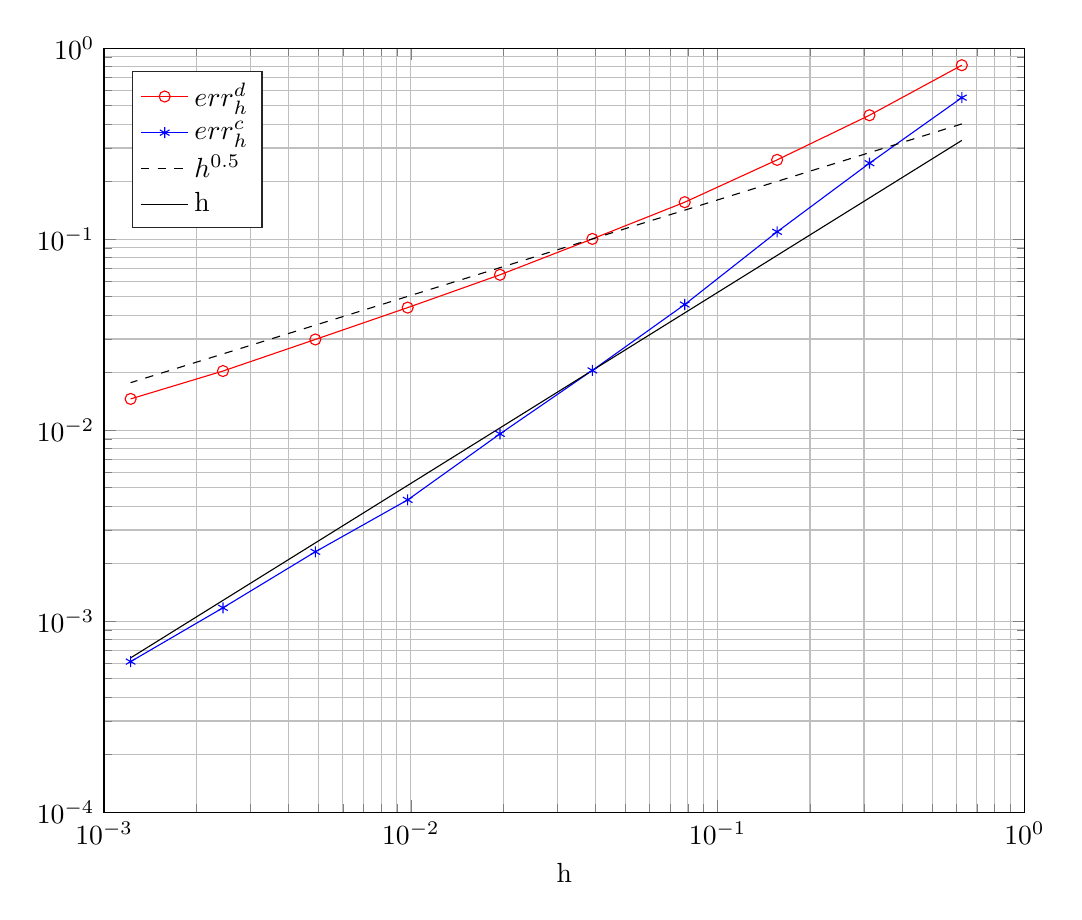
\begin{tikzpicture}

\begin{axis}[%
width=4.602in,
height=3.82in,
at={(0.772in,0.516in)},
scale only axis,
xmode=log,
xmin=0.001,
xmax=1,
xminorticks=true,
xlabel={h},
xmajorgrids,
xminorgrids,
ymode=log,
ymin=0.0001,
ymax=1,
yminorticks=true,
ymajorgrids,
yminorgrids,
axis background/.style={fill=white},
legend style={at={(0.03,0.97)},anchor=north west,legend cell align=left,align=left,draw=white!15!black}
]
\addplot [color=red,solid,mark=o,mark options={solid}]
  table[row sep=crcr]{%
0.625	0.814121166527388\\
0.3125	0.445308666527388\\
0.15625	0.260074291527388\\
0.078125	0.156160229027388\\
0.0390625	0.100300854027388\\
0.01953125	0.0650840571523877\\
0.009765625	0.0438213618398876\\
0.0048828125	0.0298496821523877\\
0.00244140625	0.0203989985586377\\
0.001220703125	0.0145757563711377\\
};
\addlegendentry{$\text{err}_\text{h}^\text{d}$};

\addplot [color=blue,solid,mark=asterisk,mark options={solid}]
  table[row sep=crcr]{%
0.625	0.550496166527388\\
0.3125	0.249839916527388\\
0.15625	0.109277416527388\\
0.078125	0.0454727290273877\\
0.0390625	0.0205547602773877\\
0.01953125	0.00956257277738766\\
0.009765625	0.00431550246488765\\
0.0048828125	0.00230768996488766\\
0.00244140625	0.00117487746488766\\
0.001220703125	0.000614086449262655\\
};
\addlegendentry{$\text{err}_\text{h}^\text{c}$};

\addplot [color=black,dashed]
  table[row sep=crcr]{%
0.625	0.401203416109551\\
0.3125	0.283693656166271\\
0.15625	0.200601708054775\\
0.078125	0.141846828083136\\
0.0390625	0.100300854027388\\
0.01953125	0.0709234140415679\\
0.009765625	0.0501504270136938\\
0.0048828125	0.0354617070207839\\
0.00244140625	0.0250752135068469\\
0.001220703125	0.017730853510392\\
};
\addlegendentry{$\text{h}^{\text{0.5}}$};

\addplot [color=black,solid]
  table[row sep=crcr]{%
0.625	0.328876164438203\\
0.3125	0.164438082219101\\
0.15625	0.0822190411095506\\
0.078125	0.0411095205547753\\
0.0390625	0.0205547602773877\\
0.01953125	0.0102773801386938\\
0.009765625	0.00513869006934691\\
0.0048828125	0.00256934503467346\\
0.00244140625	0.00128467251733673\\
0.001220703125	0.000642336258668364\\
};
\addlegendentry{h};

\end{axis}
\end{tikzpicture}% }  
        \caption{Killing boundary in $x = 1$}
        \label{fig:KillOneD}
    \end{subfigure}
    \begin{subfigure}{0.49\linewidth}
        \centering
        \resizebox{1\linewidth}{!}{% This file was created by matlab2tikz.
%
%The latest updates can be retrieved from
%  http://www.mathworks.com/matlabcentral/fileexchange/22022-matlab2tikz-matlab2tikz
%where you can also make suggestions and rate matlab2tikz.
%
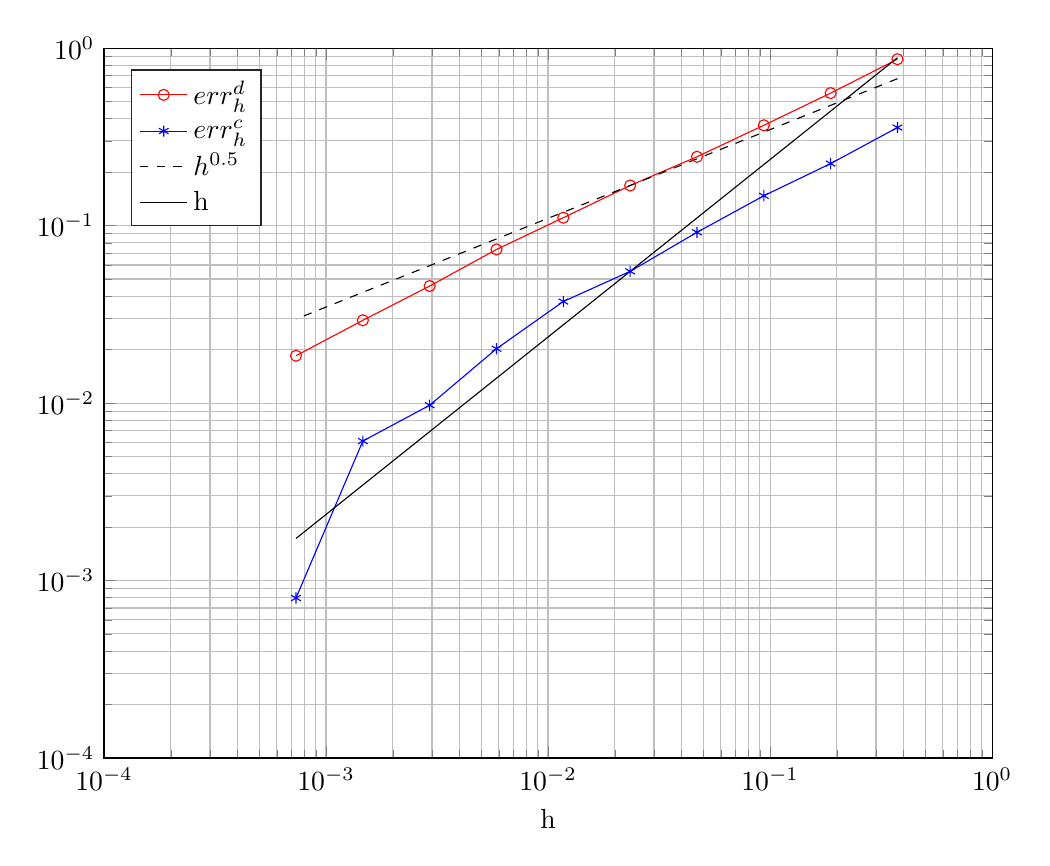
\begin{tikzpicture}

\begin{axis}[%
width=4.44in,
height=3.549in,
at={(0.745in,0.479in)},
scale only axis,
xmode=log,
xmin=0.0001,
xmax=1,
xminorticks=true,
xlabel={h},
xmajorgrids,
xminorgrids,
ymode=log,
ymin=0.0001,
ymax=1,
yminorticks=true,
ymajorgrids,
yminorgrids,
axis background/.style={fill=white},
legend style={at={(0.03,0.97)},anchor=north west,legend cell align=left,align=left,draw=white!15!black}
]
\addplot [color=red,solid,mark=o,mark options={solid}]
  table[row sep=crcr]{%
0.375	0.866448920874179\\
0.1875	0.558236420874179\\
0.09375	0.367633295874179\\
0.046875	0.244380170874179\\
0.0234375	0.168257514624179\\
0.01171875	0.110787592749179\\
0.005859375	0.0734094677491791\\
0.0029296875	0.0456410107179291\\
0.00146484375	0.0292624462648041\\
0.000732421875	0.0184820751710541\\
};
\addlegendentry{$\text{err}_\text{h}^\text{d}$};

\addplot [color=blue,solid,mark=asterisk,mark options={solid}]
  table[row sep=crcr]{%
0.375	0.357161420874179\\
0.1875	0.223680170874179\\
0.09375	0.147283295874179\\
0.046875	0.0916567333741791\\
0.0234375	0.0552278271241791\\
0.01171875	0.0373567333741791\\
0.005859375	0.0202379833741791\\
0.0029296875	0.0097233349366791\\
0.00146484375	0.00610927243667908\\
0.000732421875	0.000796943335116596\\
};
\addlegendentry{$\text{err}_\text{h}^\text{c}$};

\addplot [color=black,dashed]
  table[row sep=crcr]{%
0.375	0.673030058496717\\
0.1875	0.475904118305407\\
0.09375	0.336515029248358\\
0.046875	0.237952059152704\\
0.0234375	0.168257514624179\\
0.01171875	0.118976029576352\\
0.005859375	0.0841287573120896\\
0.0029296875	0.0594880147881759\\
0.00146484375	0.0420643786560448\\
0.000732421875	0.0297440073940879\\
};
\addlegendentry{$\text{h}^{\text{0.5}}$};

\addplot [color=black,solid]
  table[row sep=crcr]{%
0.375	0.883645233986866\\
0.1875	0.441822616993433\\
0.09375	0.220911308496716\\
0.046875	0.110455654248358\\
0.0234375	0.0552278271241791\\
0.01171875	0.0276139135620896\\
0.005859375	0.0138069567810448\\
0.0029296875	0.00690347839052239\\
0.00146484375	0.00345173919526119\\
0.000732421875	0.0017258695976306\\
};
\addlegendentry{h};

\end{axis}
\end{tikzpicture}% }  
        \caption{Reflecting boundary in $x = 1$}
        \label{fig:ReflectOneD}
    \end{subfigure}    
    \caption{Orders of convergence for DEM and CEM in the one-dimensional case.}
    \label{fig:OrdersOneD}
\end{figure}

\begin{figure}[t]
    \centering
    \begin{subfigure}{0.49\linewidth}
        \centering
        \resizebox{1\linewidth}{!}{% This file was created by matlab2tikz.
%
%The latest updates can be retrieved from
%  http://www.mathworks.com/matlabcentral/fileexchange/22022-matlab2tikz-matlab2tikz
%where you can also make suggestions and rate matlab2tikz.
%
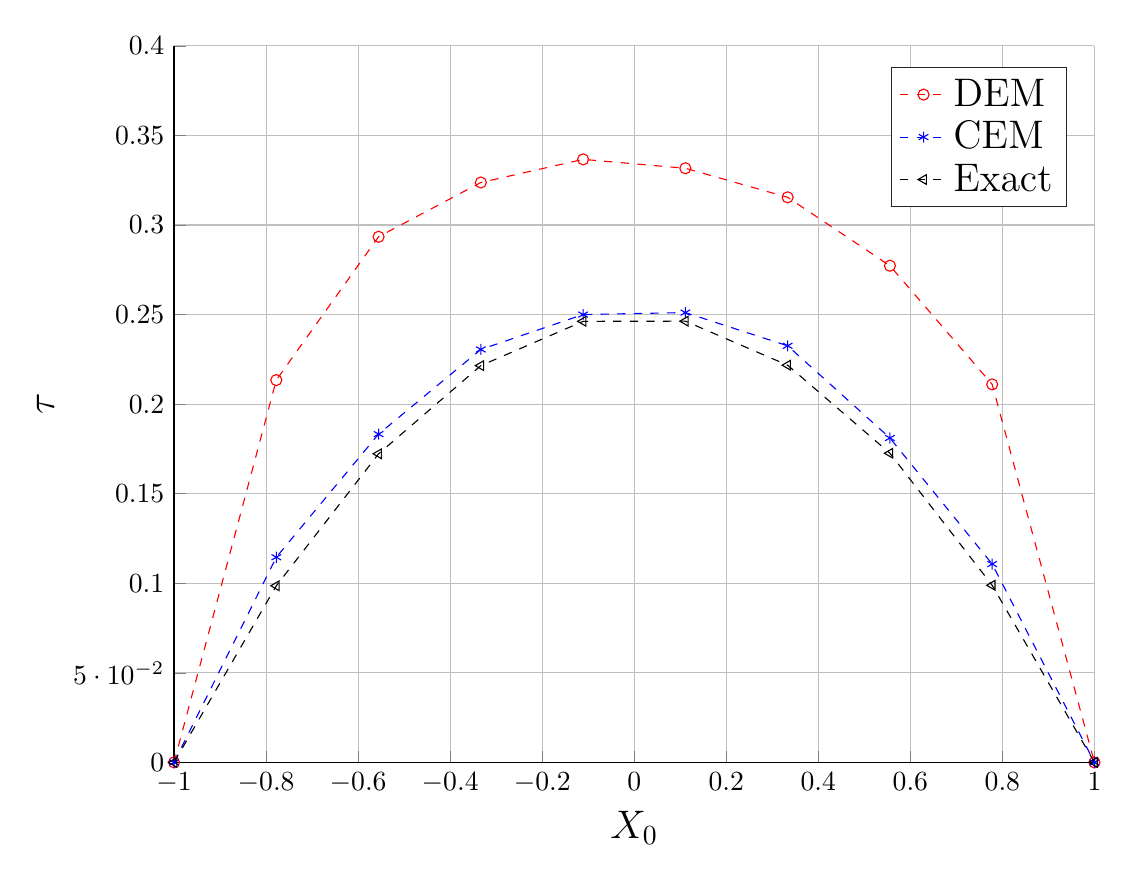
\begin{tikzpicture}

\begin{axis}[%
width=4.602in,
height=3.583in,
at={(0.772in,0.484in)},
scale only axis,
xmin=-1,
xmax=1,
xlabel={$X_0$},
xlabel style = {font = \Large},
xmajorgrids,
ymin=0,
ymax=0.4,
ylabel={$\tau$},
ylabel style = {font = \Large},
ymajorgrids,
axis background/.style={fill=white},
axis x line*=bottom,
axis y line*=left,
legend pos = north east,
legend style={legend cell align=left,align=left,draw=white!15!black,font=\Large}
]
\addplot [color=red,dashed,mark=o,mark options={solid}]
  table[row sep=crcr]{%
-1	0\\
-0.777777777777778	0.213421875\\
-0.555555555555556	0.2934140625\\
-0.333333333333333	0.3236953125\\
-0.111111111111111	0.336609375\\
0.111111111111111	0.331640625\\
0.333333333333333	0.315421875\\
0.555555555555556	0.2772421875\\
0.777777777777778	0.2110078125\\
1	0\\
};
\addlegendentry{DEM};

\addplot [color=blue,dashed,mark=asterisk,mark options={solid}]
  table[row sep=crcr]{%
-1	0\\
-0.777777777777778	0.114515625\\
-0.555555555555556	0.1832578125\\
-0.333333333333333	0.2305078125\\
-0.111111111111111	0.249984375\\
0.111111111111111	0.2510859375\\
0.333333333333333	0.232546875\\
0.555555555555556	0.181078125\\
0.777777777777778	0.11071875\\
1	0\\
};
\addlegendentry{CEM};

\addplot [color=black,dashed,mark=triangle,mark options={solid,rotate=90}]
  table[row sep=crcr]{%
-1	0\\
-0.777777777777778	0.0986011931395157\\
-0.555555555555556	0.172254291984329\\
-0.333333333333333	0.221472162307402\\
-0.111111111111111	0.246204174763737\\
0.111111111111111	0.2462957329545\\
0.333333333333333	0.221719125026098\\
0.555555555555556	0.172574095814315\\
0.777777777777778	0.0988572350577004\\
1	0\\
};
\addlegendentry{Exact};

\end{axis}
\end{tikzpicture}%
 }  
        \caption{Killing boundary in $x = 1$}
        \label{fig:ApproxOneD}
    \end{subfigure}
    \begin{subfigure}{0.49\linewidth}
        \centering
        \resizebox{1\linewidth}{!}{% This file was created by matlab2tikz.
%
%The latest updates can be retrieved from
%  http://www.mathworks.com/matlabcentral/fileexchange/22022-matlab2tikz-matlab2tikz
%where you can also make suggestions and rate matlab2tikz.
%
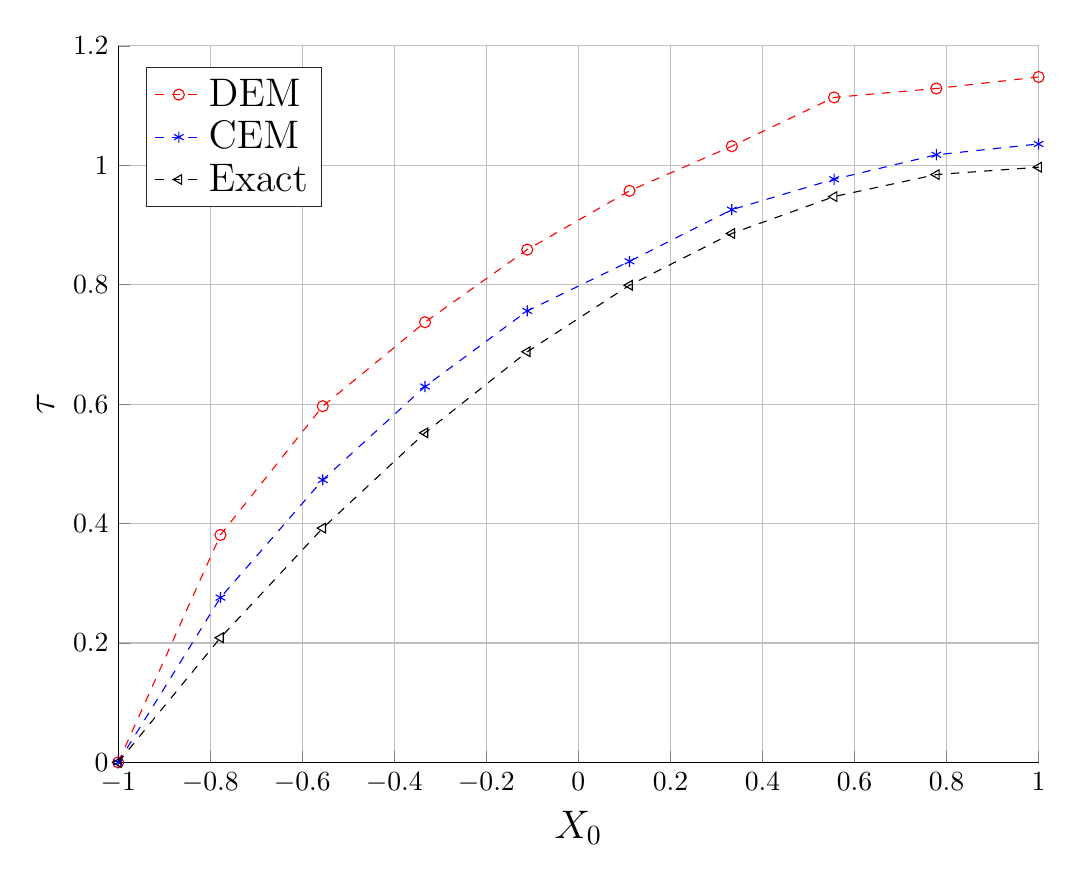
\begin{tikzpicture}

\begin{axis}[%
width=4.602in,
height=3.583in,
at={(0.772in,0.484in)},
scale only axis,
xmin=-1,
xmax=1,
xlabel={$X_0$},
xlabel style={font=\Large},
xmajorgrids,
ymin=0,
ymax=1.2,
ylabel={$\tau$},
ylabel style={font=\Large},
ymajorgrids,
axis background/.style={fill=white},
axis x line*=bottom,
axis y line*=left,
legend style={at={(0.03,0.97)},anchor=north west,legend cell align=left,align=left,draw=white!15!black,font=\Large}
]
\addplot [color=red,dashed,mark=o,mark options={solid}]
  table[row sep=crcr]{%
-1	0\\
-0.777777777777778	0.3809765625\\
-0.555555555555556	0.5964609375\\
-0.333333333333333	0.73715625\\
-0.111111111111111	0.8587265625\\
0.111111111111111	0.9571171875\\
0.333333333333333	1.031859375\\
0.555555555555556	1.113609375\\
0.777777777777778	1.1285390625\\
1	1.1478046875\\
};
\addlegendentry{DEM};

\addplot [color=blue,dashed,mark=asterisk,mark options={solid}]
  table[row sep=crcr]{%
-1	0\\
-0.777777777777778	0.275953125\\
-0.555555555555556	0.4729921875\\
-0.333333333333333	0.629484375\\
-0.111111111111111	0.7560703125\\
0.111111111111111	0.8390625\\
0.333333333333333	0.9255703125\\
0.555555555555556	0.976546875\\
0.777777777777778	1.017515625\\
1	1.035609375\\
};
\addlegendentry{CEM};

\addplot [color=black,dashed,mark=triangle,mark options={solid,rotate=90}]
  table[row sep=crcr]{%
-1	0\\
-0.777777777777778	0.208777054487475\\
-0.555555555555556	0.392333503315235\\
-0.333333333333333	0.551939853868488\\
-0.111111111111111	0.687661056545228\\
0.111111111111111	0.79906851214989\\
0.333333333333333	0.885727939207175\\
0.555555555555556	0.947463001823471\\
0.777777777777778	0.984384604394486\\
1	0.996687130893952\\
};
\addlegendentry{Exact};

\end{axis}
\end{tikzpicture}%
 }  
        \caption{Reflecting boundary in $x = 1$}
        \label{fig:ApproxOneD}
    \end{subfigure}    
    \caption{Approximation of $\tau$ for the discrete and continuous EM method in the one-dimensional case.}
    \label{fig:ApproxOneD}
\end{figure}

\begin{figure}[t]
        \centering
        \resizebox{0.6\linewidth}{!}{% This file was created by matlab2tikz.
%
%The latest updates can be retrieved from
%  http://www.mathworks.com/matlabcentral/fileexchange/22022-matlab2tikz-matlab2tikz
%where you can also make suggestions and rate matlab2tikz.
%
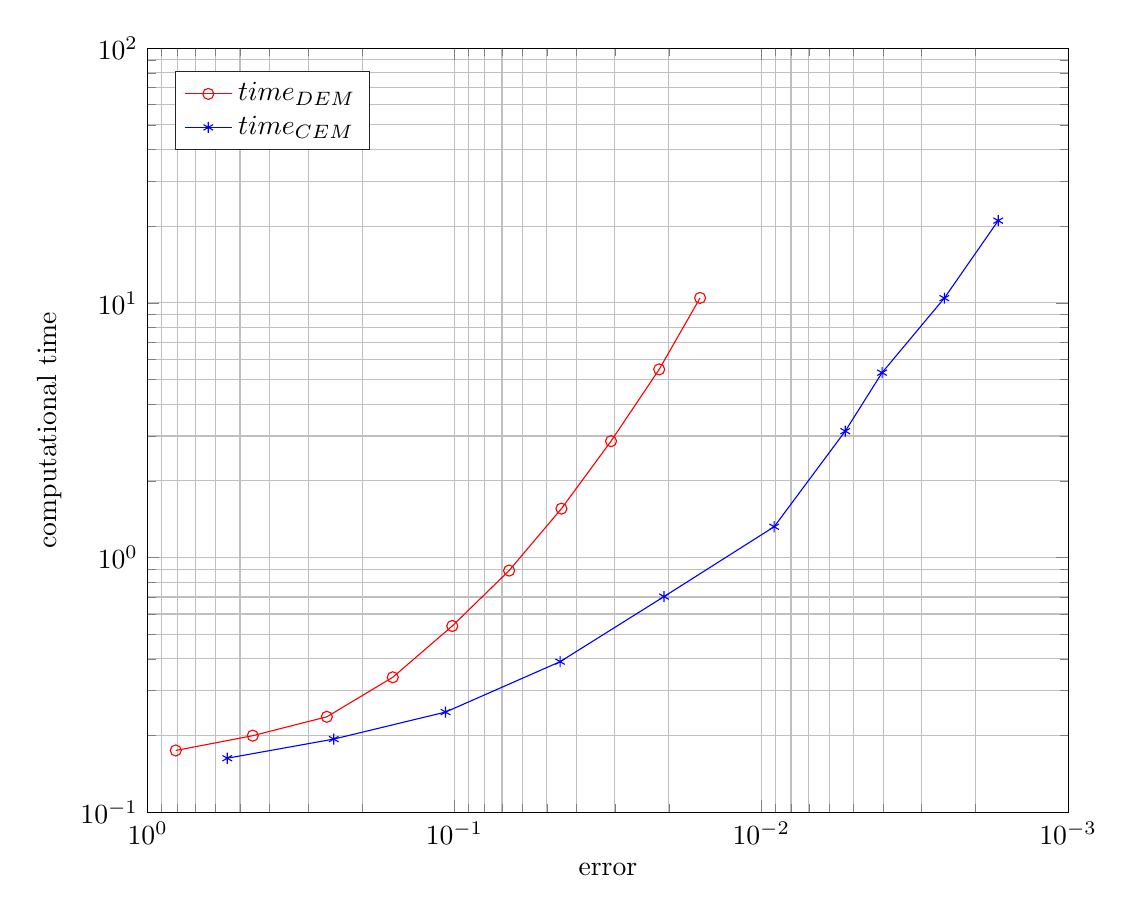
\begin{tikzpicture}

\begin{axis}[%
width=4.602in,
height=3.82in,
at={(0.772in,0.516in)},
scale only axis,
x dir=reverse,
xmode=log,
xmin=0.001,
xmax=1,
xminorticks=true,
xlabel={error},
xmajorgrids,
xminorgrids,
ymode=log,
ymin=0.1,
ymax=100,
yminorticks=true,
ylabel={computational time},
ymajorgrids,
yminorgrids,
axis background/.style={fill=white},
legend style={at={(0.03,0.97)},anchor=north west,legend cell align=left,align=left,draw=white!15!black}
]
\addplot [color=red,solid,mark=o,mark options={solid}]
  table[row sep=crcr]{%
0.809808666527388	0.174713\\
0.454308666527388	0.199743\\
0.260652416527388	0.23684\\
0.158902416527388	0.338576\\
0.101648510277388	0.538431\\
0.0663692134023876	0.888358\\
0.0448057368398877	1.555625\\
0.0308814204336377	2.863223\\
0.0215156977773877	5.478668\\
0.0158268550039502	10.454508\\
};
\addlegendentry{$\text{time}_{\text{DEM}}$};

\addplot [color=blue,solid,mark=asterisk,mark options={solid}]
  table[row sep=crcr]{%
0.550433666527388	0.162876\\
0.247433666527388	0.193649\\
0.106918041527388	0.247227\\
0.0452461665273877	0.390013\\
0.0207461665273877	0.702369\\
0.00907819777738766	1.320507\\
0.00532429152738766	3.134469\\
0.00403864699613767	5.317267\\
0.00253132277738766	10.432115\\
0.00168928176176265	21.021666\\
};
\addlegendentry{$\text{time}_{\text{CEM}}$};

\end{axis}
\end{tikzpicture}% }  
        \caption{error vs work plot for DEM and CEM.}
        \label{fig:CompTime}
\end{figure}


\vspace{2mm}
\noindent\textbf{Rough case.} We consider the same domain $D$ as above, $T = 5$ and $g = \sigma = 3$. We consider $V$ to be piecewise linear, so that $f = -dV$ is piecewise constant. In particular, we choose the following form for $V$
\begin{equation}\label{eq:FunctionsOneDRough}
V = 0.1 
\begin{cases}
	 -2x -1 & x < -0.5, \\
	 4x + 2 & -0.5 \leq x < 0, \\
	 -2x + 2 &  0 \leq x < 0.5, \\
	 4x - 1 & x \geq 0.5.
\end{cases}
\end{equation}
This is a linear interpolation of the function $V$ we used in the smooth case above in the points $\{-1,-0.5,0,0.5,1\}$ (Figure \ref{fig:PlotsVSmoothRough}). This case is of particular interest, since if the function $f$ is the result of a numerical method on a $PDE$, it could not be smooth as in the previous case. We perform DEM and CEM with the same parameters as before, \textit{i.e.}, $M = 10000, N = 2^i,i=3,\dots,12$. In Figure \ref{fig:OrdersOneDRough} it is possible to remark that the rate of convergence of DEM is unvaried with respect to the previous case. The CEM method experiences a slight decrease in the order of convergence with respect to the smooth case.

\begin{figure}[t]
        \centering
        \resizebox{0.6\linewidth}{!}{% This file was created by matlab2tikz.
%
%The latest updates can be retrieved from
%  http://www.mathworks.com/matlabcentral/fileexchange/22022-matlab2tikz-matlab2tikz
%where you can also make suggestions and rate matlab2tikz.
%
\definecolor{mycolor1}{rgb}{0.00000,0.44700,0.74100}%
%
\begin{tikzpicture}

\begin{axis}[%
width=4.521in,
height=3.566in,
at={(0.758in,0.481in)},
scale only axis,
xmin=-1,
xmax=1,
xmajorgrids,
ymin=-1.5,
ymax=2,
ymajorgrids,
axis background/.style={fill=white},
legend style={at={(0.03,0.97)},anchor=north west,legend cell align=left,align=left,draw=white!15!black}
]
\addplot [color=mycolor1,solid,line width=2.0pt]
  table[row sep=crcr]{%
-1	0.1\\
-0.999	0.0985039968008\\
-0.998	0.0970159744128\\
-0.997	0.0955359136648\\
-0.996	0.0940637954048\\
-0.995	0.0925996004999999\\
-0.994	0.0911433098368\\
-0.993	0.0896949043208001\\
-0.992	0.0882543648768\\
-0.991	0.0868216724488\\
-0.99	0.085396808\\
-0.989	0.0839797525128\\
-0.988	0.0825704869887999\\
-0.987	0.0811689924488\\
-0.986	0.0797752499328\\
-0.985	0.0783892405\\
-0.984	0.0770109452288\\
-0.983	0.0756403452168\\
-0.982	0.0742774215808\\
-0.981	0.0729221554567999\\
-0.98	0.0715745280000001\\
-0.979	0.0702345203847999\\
-0.978	0.0689021138048\\
-0.977	0.0675772894728\\
-0.976	0.0662600286208\\
-0.975	0.0649503124999999\\
-0.974	0.0636481223808\\
-0.973	0.0623534395528\\
-0.972	0.0610662453247999\\
-0.971	0.0597865210248\\
-0.97	0.058514248\\
-0.969	0.0572494076168\\
-0.968	0.0559919812607999\\
-0.967	0.0547419503367999\\
-0.966	0.0534992962688\\
-0.965	0.0522640005\\
-0.964	0.0510360444928\\
-0.963	0.0498154097288\\
-0.962	0.0486020777088\\
-0.961	0.0473960299528\\
-0.96	0.0461972479999999\\
-0.959	0.0450057134087999\\
-0.958	0.0438214077568\\
-0.957	0.0426443126408\\
-0.956	0.0414744096767999\\
-0.955	0.0403116804999999\\
-0.954	0.0391561067647999\\
-0.953	0.0380076701448\\
-0.952	0.0368663523328\\
-0.951	0.0357321350408\\
-0.95	0.0346049999999999\\
-0.949	0.0334849289608\\
-0.948	0.0323719036927999\\
-0.947	0.0312659059848\\
-0.946	0.0301669176448\\
-0.945	0.0290749205\\
-0.944	0.0279898963967999\\
-0.943	0.0269118272007999\\
-0.942	0.0258406947967999\\
-0.941	0.0247764810888\\
-0.94	0.0237191679999999\\
-0.939	0.0226687374728001\\
-0.938	0.0216251714688\\
-0.937	0.0205884519688001\\
-0.936	0.0195585609728\\
-0.935	0.0185354805000001\\
-0.934	0.0175191925887999\\
-0.933	0.0165096792968001\\
-0.932	0.0155069227008\\
-0.931	0.0145109048968\\
-0.93	0.0135216079999999\\
-0.929	0.0125390141448001\\
-0.928	0.0115631054848\\
-0.927	0.0105938641928\\
-0.926	0.00963127246079996\\
-0.925	0.00867531250000002\\
-0.924	0.0077259665408\\
-0.923	0.00678321683280005\\
-0.922	0.00584704564480005\\
-0.921	0.00491743526480006\\
-0.92	0.00399436800000004\\
-0.919	0.00307782617679995\\
-0.918	0.00216779214080001\\
-0.917	0.0012642482568\\
-0.916	0.00036717690880006\\
-0.915	-0.000523439499999956\\
-0.914	-0.00140761854719993\\
-0.913	-0.00228537779120002\\
-0.912	-0.00315673477119995\\
-0.911	-0.00402170700719995\\
-0.91	-0.00488031199999996\\
-0.909	-0.00573256723119995\\
-0.908	-0.00657849016320005\\
-0.907	-0.00741809823919999\\
-0.906	-0.00825140888319997\\
-0.905	-0.0090784395\\
-0.904	-0.00989920747520001\\
-0.903	-0.0107137301752\\
-0.902	-0.0115220249471999\\
-0.901	-0.0123241091191999\\
-0.9	-0.0131199999999999\\
-0.899	-0.0139097148792001\\
-0.898	-0.0146932710272\\
-0.897	-0.0154706856952\\
-0.896	-0.0162419761152\\
-0.895	-0.0170071594999999\\
-0.894	-0.0177662530432\\
-0.893	-0.0185192739192\\
-0.892	-0.0192662392832\\
-0.891	-0.0200071662712\\
-0.89	-0.020742072\\
-0.889	-0.0214709735672001\\
-0.888	-0.0221938880512\\
-0.887	-0.0229108325112\\
-0.886	-0.0236218239872\\
-0.885	-0.0243268795000001\\
-0.884	-0.0250260160512\\
-0.883	-0.0257192506231999\\
-0.882	-0.0264066001792\\
-0.881	-0.0270880816632\\
-0.88	-0.027763712\\
-0.879	-0.0284335080952\\
-0.878	-0.0290974868352\\
-0.877	-0.0297556650871999\\
-0.876	-0.0304080596991999\\
-0.875	-0.0310546875\\
-0.874	-0.0316955652992\\
-0.873	-0.0323307098872\\
-0.872	-0.0329601380351999\\
-0.871	-0.0335838664952\\
-0.87	-0.0342019120000001\\
-0.869	-0.0348142912632\\
-0.868	-0.0354210209791999\\
-0.867	-0.0360221178232\\
-0.866	-0.0366175984512\\
-0.865	-0.0372074795\\
-0.864	-0.0377917775872\\
-0.863	-0.0383705093112\\
-0.862	-0.0389436912512\\
-0.861	-0.0395113399672\\
-0.86	-0.040073472\\
-0.859	-0.0406301038712001\\
-0.858	-0.0411812520832\\
-0.857	-0.0417269331192001\\
-0.856	-0.0422671634432\\
-0.855	-0.0428019595\\
-0.854	-0.0433313377152\\
-0.853	-0.0438553144951999\\
-0.852	-0.0443739062272\\
-0.851	-0.0448871292792\\
-0.85	-0.045395\\
-0.849	-0.0458975347192\\
-0.848	-0.0463947497472\\
-0.847	-0.0468866613752\\
-0.846	-0.0473732858752\\
-0.845	-0.0478546395\\
-0.844	-0.0483307384832\\
-0.843	-0.0488015990392\\
-0.842	-0.0492672373632\\
-0.841	-0.0497276696312\\
-0.84	-0.050182912\\
-0.839	-0.0506329806072\\
-0.838	-0.0510778915712001\\
-0.837	-0.0515176609912\\
-0.836	-0.0519523049472\\
-0.835	-0.0523818395000001\\
-0.834	-0.0528062806912\\
-0.833	-0.0532256445432001\\
-0.832	-0.0536399470592\\
-0.831	-0.0540492042232001\\
-0.83	-0.054453432\\
-0.829	-0.0548526463352\\
-0.828	-0.0552468631552\\
-0.827	-0.0556360983672\\
-0.826	-0.0560203678592\\
-0.825	-0.0563996875\\
-0.824	-0.0567740731392\\
-0.823	-0.0571435406072001\\
-0.822	-0.0575081057152\\
-0.821	-0.0578677842552\\
-0.82	-0.058222592\\
-0.819	-0.0585725447032\\
-0.818	-0.0589176580992\\
-0.817	-0.0592579479032\\
-0.816	-0.0595934298112\\
-0.815	-0.0599241195000001\\
-0.814	-0.0602500326272\\
-0.813	-0.0605711848312001\\
-0.812	-0.0608875917311999\\
-0.811	-0.0611992689272\\
-0.81	-0.061506232\\
-0.809	-0.0618084965112\\
-0.808	-0.0621060780032\\
-0.807	-0.0623989919992\\
-0.806	-0.0626872540032\\
-0.805	-0.0629708795\\
-0.804	-0.0632498839552\\
-0.803	-0.0635242828152\\
-0.802	-0.0637940915072\\
-0.801	-0.0640593254392\\
-0.8	-0.06432\\
-0.799	-0.0645761305592\\
-0.798	-0.0648277324672\\
-0.797	-0.0650748210552\\
-0.796	-0.0653174116352\\
-0.795	-0.0655555195\\
-0.794	-0.0657891599232\\
-0.793	-0.0660183481592\\
-0.792	-0.0662430994431999\\
-0.791	-0.0664634289912\\
-0.79	-0.066679352\\
-0.789	-0.0668908836472001\\
-0.788	-0.0670980390912\\
-0.787	-0.0673008334712\\
-0.786	-0.0674992819072\\
-0.785	-0.0676933995\\
-0.784	-0.0678832013312\\
-0.783	-0.0680687024631999\\
-0.782	-0.0682499179392\\
-0.781	-0.0684268627832001\\
-0.78	-0.068599552\\
-0.779	-0.0687680005752\\
-0.778	-0.0689322234752\\
-0.777	-0.0690922356472\\
-0.776	-0.0692480520192\\
-0.775	-0.0693996875\\
-0.774	-0.0695471569792\\
-0.773	-0.0696904753272\\
-0.772	-0.0698296573952001\\
-0.771	-0.0699647180152\\
-0.77	-0.070095672\\
-0.769	-0.0702225341432\\
-0.768	-0.0703453192192\\
-0.767	-0.0704640419832\\
-0.766	-0.0705787171712\\
-0.765	-0.0706893595\\
-0.764	-0.0707959836672\\
-0.763	-0.0708986043512\\
-0.762	-0.0709972362112\\
-0.761	-0.0710918938872\\
-0.76	-0.071182592\\
-0.759	-0.0712693451512001\\
-0.758	-0.0713521679232\\
-0.757	-0.0714310748792\\
-0.756	-0.0715060805632001\\
-0.755	-0.0715771995\\
-0.754	-0.0716444461952\\
-0.753	-0.0717078351352\\
-0.752	-0.0717673807872\\
-0.751	-0.0718230975992\\
-0.75	-0.071875\\
-0.749	-0.0719231023992\\
-0.748	-0.0719674191872001\\
-0.747	-0.0720079647352\\
-0.746	-0.0720447533952\\
-0.745	-0.0720777995\\
-0.744	-0.0721071173632001\\
-0.743	-0.0721327212792\\
-0.742	-0.0721546255232\\
-0.741	-0.0721728443512001\\
-0.74	-0.072187392\\
-0.739	-0.0721982826872\\
-0.738	-0.0722055306112\\
-0.737	-0.0722091499512\\
-0.736	-0.0722091548672\\
-0.735	-0.0722055595\\
-0.734	-0.0721983779712\\
-0.733	-0.0721876243832\\
-0.732	-0.0721733128192\\
-0.731	-0.0721554573432\\
-0.73	-0.072134072\\
-0.729	-0.0721091708152\\
-0.728	-0.0720807677952\\
-0.727	-0.0720488769272\\
-0.726	-0.0720135121792\\
-0.725	-0.0719746875\\
-0.724	-0.0719324168192\\
-0.723	-0.0718867140472\\
-0.722	-0.0718375930752\\
-0.721	-0.0717850677752\\
-0.72	-0.071729152\\
-0.719	-0.0716698595832\\
-0.718	-0.0716072043392\\
-0.717	-0.0715412000632\\
-0.716	-0.0714718605312\\
-0.715	-0.0713991995\\
-0.714	-0.0713232307072\\
-0.713	-0.0712439678712\\
-0.712	-0.0711614246912\\
-0.711	-0.0710756148472\\
-0.71	-0.070986552\\
-0.709	-0.0708942497912001\\
-0.708	-0.0707987218432\\
-0.707	-0.0706999817592\\
-0.706	-0.0705980431232\\
-0.705	-0.0704929195\\
-0.704	-0.0703846244352\\
-0.703	-0.0702731714552\\
-0.702	-0.0701585740672\\
-0.701	-0.0700408457592\\
-0.7	-0.06992\\
-0.699	-0.0697960502392\\
-0.698	-0.0696690099072\\
-0.697	-0.0695388924152\\
-0.696	-0.0694057111552\\
-0.695	-0.0692694795000001\\
-0.694	-0.0691302108032\\
-0.693	-0.0689879183992\\
-0.692	-0.0688426156032\\
-0.691	-0.0686943157112\\
-0.69	-0.068543032\\
-0.689	-0.0683887777272\\
-0.688	-0.0682315661312\\
-0.687	-0.0680714104312\\
-0.686	-0.0679083238272\\
-0.685	-0.0677423195\\
-0.684	-0.0675734106112\\
-0.683	-0.0674016103032001\\
-0.682	-0.0672269316992\\
-0.681	-0.0670493879032001\\
-0.68	-0.066868992\\
-0.679	-0.0666857570552001\\
-0.678	-0.0664996961152\\
-0.677	-0.0663108222072\\
-0.676	-0.0661191483392\\
-0.675	-0.0659246875\\
-0.674	-0.0657274526592\\
-0.673	-0.0655274567672001\\
-0.672	-0.0653247127552\\
-0.671	-0.0651192335352\\
-0.67	-0.064911032\\
-0.669	-0.0647001210232\\
-0.668	-0.0644865134592\\
-0.667	-0.0642702221432\\
-0.666	-0.0640512598912\\
-0.665	-0.0638296395\\
-0.664	-0.0636053737472\\
-0.663	-0.0633784753912\\
-0.662	-0.0631489571712\\
-0.661	-0.0629168318072\\
-0.66	-0.062682112\\
-0.659	-0.0624448104312\\
-0.658	-0.0622049397632\\
-0.657	-0.0619625126392\\
-0.656	-0.0617175416832\\
-0.655	-0.0614700395\\
-0.654	-0.0612200186752\\
-0.653	-0.0609674917752\\
-0.652	-0.0607124713472\\
-0.651	-0.0604549699192\\
-0.65	-0.060195\\
-0.649	-0.0599325740792\\
-0.648	-0.0596677046272\\
-0.647	-0.0594004040952\\
-0.646	-0.0591306849152\\
-0.645	-0.0588585595\\
-0.644	-0.0585840402432\\
-0.643	-0.0583071395192\\
-0.642	-0.0580278696832\\
-0.641	-0.0577462430712\\
-0.64	-0.057462272\\
-0.639	-0.0571759687672\\
-0.638	-0.0568873456512\\
-0.637	-0.0565964149112\\
-0.636	-0.0563031887872\\
-0.635	-0.0560076795\\
-0.634	-0.0557098992512\\
-0.633	-0.0554098602232\\
-0.632	-0.0551075745792\\
-0.631	-0.0548030544632\\
-0.63	-0.054496312\\
-0.629	-0.0541873592952\\
-0.628	-0.0538762084352\\
-0.627	-0.0535628714872\\
-0.626	-0.0532473604992\\
-0.625	-0.0529296875\\
-0.624	-0.0526098644992\\
-0.623	-0.0522879034872\\
-0.622	-0.0519638164352\\
-0.621	-0.0516376152952\\
-0.62	-0.051309312\\
-0.619	-0.0509789184632\\
-0.618	-0.0506464465792\\
-0.617	-0.0503119082232\\
-0.616	-0.0499753152512\\
-0.615	-0.0496366795\\
-0.614	-0.0492960127872\\
-0.613	-0.0489533269112\\
-0.612	-0.0486086336512\\
-0.611	-0.0482619447672\\
-0.61	-0.047913272\\
-0.609	-0.0475626270712\\
-0.608	-0.0472100216832\\
-0.607	-0.0468554675192\\
-0.606	-0.0464989762432\\
-0.605	-0.0461405595\\
-0.604	-0.0457802289152\\
-0.603	-0.0454179960952\\
-0.602	-0.0450538726272\\
-0.601	-0.0446878700792\\
-0.6	-0.04432\\
-0.599	-0.0439502739192\\
-0.598	-0.0435787033472\\
-0.597	-0.0432052997752\\
-0.596	-0.0428300746752\\
-0.595	-0.0424530395\\
-0.594	-0.0420742056832\\
-0.593	-0.0416935846392\\
-0.592	-0.0413111877632\\
-0.591	-0.0409270264312\\
-0.59	-0.040541112\\
-0.589	-0.0401534558072\\
-0.588	-0.0397640691712\\
-0.587	-0.0393729633912\\
-0.586	-0.0389801497472\\
-0.585	-0.0385856395\\
-0.584	-0.0381894438912\\
-0.583	-0.0377915741432\\
-0.582	-0.0373920414592\\
-0.581	-0.0369908570232\\
-0.58	-0.036588032\\
-0.579	-0.0361835775352\\
-0.578	-0.0357775047552001\\
-0.577	-0.0353698247672\\
-0.576	-0.0349605486592\\
-0.575	-0.0345496875\\
-0.574	-0.0341372523392001\\
-0.573	-0.0337232542072\\
-0.572	-0.0333077041152\\
-0.571	-0.0328906130552\\
-0.57	-0.0324719920000001\\
-0.569	-0.0320518519032\\
-0.568	-0.0316302036992\\
-0.567	-0.0312070583032\\
-0.566	-0.0307824266112\\
-0.565	-0.0303563195\\
-0.564	-0.0299287478272\\
-0.563	-0.0294997224312\\
-0.562	-0.0290692541312001\\
-0.561	-0.0286373537272\\
-0.56	-0.028204032\\
-0.559	-0.0277692997112\\
-0.558	-0.0273331676032001\\
-0.557	-0.0268956463992\\
-0.556	-0.0264567468032\\
-0.555	-0.0260164795\\
-0.554	-0.0255748551552\\
-0.553	-0.0251318844152\\
-0.552	-0.0246875779072\\
-0.551	-0.0242419462392\\
-0.55	-0.023795\\
-0.549	-0.0233467497592\\
-0.548	-0.0228972060672001\\
-0.547	-0.0224463794552\\
-0.546	-0.0219942804352\\
-0.545	-0.0215409194999999\\
-0.544	-0.0210863071232\\
-0.543	-0.0206304537592\\
-0.542	-0.0201733698432\\
-0.541	-0.0197150657912\\
-0.54	-0.019255552\\
-0.539	-0.0187948388472\\
-0.538	-0.0183329366912\\
-0.537	-0.0178698558712\\
-0.536	-0.0174056067072\\
-0.535	-0.0169401994999999\\
-0.534	-0.0164736445312\\
-0.533	-0.0160059520632\\
-0.532	-0.0155371323392\\
-0.531	-0.0150671955831999\\
-0.53	-0.014596152\\
-0.529	-0.0141240117752\\
-0.528	-0.0136507850752\\
-0.527	-0.0131764820471999\\
-0.526	-0.0127011128192001\\
-0.525	-0.0122246875\\
-0.524	-0.0117472161792\\
-0.523	-0.0112687089272\\
-0.522	-0.0107891757952\\
-0.521	-0.0103086268152\\
-0.52	-0.00982707200000004\\
-0.519	-0.00934452134320001\\
-0.518	-0.00886098481920001\\
-0.517	-0.00837647238320001\\
-0.516	-0.00789099397120001\\
-0.515	-0.00740455949999999\\
-0.514	-0.00691717886719996\\
-0.513	-0.00642886195119998\\
-0.512	-0.0059396186112\\
-0.511	-0.00544945868719999\\
-0.51	-0.00495839199999999\\
-0.509	-0.00446642835120001\\
-0.508	-0.00397357752320002\\
-0.507	-0.00347984927920004\\
-0.506	-0.00298525336319999\\
-0.505	-0.00248979949999999\\
-0.504	-0.00199349739520001\\
-0.503	-0.00149635673519999\\
-0.502	-0.000998387187200001\\
-0.501	-0.000499598399199952\\
-0.5	0\\
-0.499	0.000500398400799984\\
-0.498	0.00100158721279999\\
-0.497	0.00150355686479999\\
-0.496	0.00200629780480002\\
-0.495	0.00250980049999998\\
-0.494	0.0030140554368\\
-0.493	0.00351905312080003\\
-0.492	0.0040247840768\\
-0.491	0.0045312388488\\
-0.49	0.00503840800000002\\
-0.489	0.00554628211280002\\
-0.488	0.00605485178880001\\
-0.487	0.00656410764880002\\
-0.486	0.00707404033279999\\
-0.485	0.00758464050000001\\
-0.484	0.0080958988288\\
-0.483	0.0086078060168\\
-0.482	0.00912035278080001\\
-0.481	0.00963352985679999\\
-0.48	0.010147328\\
-0.479	0.0106617379848\\
-0.478	0.0111767506048\\
-0.477	0.0116923566728\\
-0.476	0.0122085470208\\
-0.475	0.0127253125\\
-0.474	0.0132426439808\\
-0.473	0.0137605323528\\
-0.472	0.0142789685248\\
-0.471	0.0147979434248\\
-0.47	0.015317448\\
-0.469	0.0158374732168\\
-0.468	0.0163580100608\\
-0.467	0.0168790495368\\
-0.466	0.0174005826688\\
-0.465	0.0179226005\\
-0.464	0.0184450940928\\
-0.463	0.0189680545288\\
-0.462	0.0194914729088\\
-0.461	0.0200153403528\\
-0.46	0.020539648\\
-0.459	0.0210643870088\\
-0.458	0.0215895485568\\
-0.457	0.0221151238408\\
-0.456	0.0226411040768\\
-0.455	0.0231674805\\
-0.454	0.0236942443648\\
-0.453	0.0242213869448\\
-0.452	0.0247488995328\\
-0.451	0.0252767734408\\
-0.45	0.025805\\
-0.449	0.0263335705608001\\
-0.448	0.0268624764928\\
-0.447	0.0273917091848\\
-0.446	0.0279212600448\\
-0.445	0.0284511205\\
-0.444	0.0289812819968\\
-0.443	0.0295117360008\\
-0.442	0.0300424739968\\
-0.441	0.0305734874888\\
-0.44	0.031104768\\
-0.439	0.0316363070728\\
-0.438	0.0321680962688\\
-0.437	0.0327001271688\\
-0.436	0.0332323913728\\
-0.435	0.0337648805\\
-0.434	0.0342975861888\\
-0.433	0.0348305000968\\
-0.432	0.0353636139008\\
-0.431	0.0358969192968\\
-0.43	0.036430408\\
-0.429	0.0369640717448\\
-0.428	0.0374979022848\\
-0.427	0.0380318913928\\
-0.426	0.0385660308608\\
-0.425	0.0391003125\\
-0.424	0.0396347281408\\
-0.423	0.0401692696328\\
-0.422	0.0407039288448\\
-0.421	0.0412386976648\\
-0.42	0.041773568\\
-0.419	0.0423085317768\\
-0.418	0.0428435809408\\
-0.417	0.0433787074568\\
-0.416	0.0439139033088\\
-0.415	0.0444491605\\
-0.414	0.0449844710528\\
-0.413	0.0455198270088\\
-0.412	0.0460552204288\\
-0.411	0.0465906433928\\
-0.41	0.047126088\\
-0.409	0.0476615463688\\
-0.408	0.0481970106368\\
-0.407	0.0487324729608\\
-0.406	0.0492679255168\\
-0.405	0.0498033605\\
-0.404	0.0503387701248\\
-0.403	0.0508741466248\\
-0.402	0.0514094822528\\
-0.401	0.0519447692808\\
-0.4	0.05248\\
-0.399	0.0530151667208\\
-0.398	0.0535502617728\\
-0.397	0.0540852775048\\
-0.396	0.0546202062848\\
-0.395	0.0551550405\\
-0.394	0.0556897725568\\
-0.393	0.0562243948808\\
-0.392	0.0567588999168\\
-0.391	0.0572932801288\\
-0.39	0.057827528\\
-0.389	0.0583616360328\\
-0.388	0.0588955967488\\
-0.387	0.0594294026888\\
-0.386	0.0599630464128\\
-0.385	0.0604965205\\
-0.384	0.0610298175488\\
-0.383	0.0615629301768\\
-0.382	0.0620958510208\\
-0.381	0.0626285727368\\
-0.38	0.063161088\\
-0.379	0.0636933895048\\
-0.378	0.0642254699648\\
-0.377	0.0647573221128\\
-0.376	0.0652889387008\\
-0.375	0.0658203125\\
-0.374	0.0663514363008\\
-0.373	0.0668823029128\\
-0.372	0.0674129051648\\
-0.371	0.0679432359048\\
-0.37	0.068473288\\
-0.369	0.0690030543368\\
-0.368	0.0695325278208\\
-0.367	0.0700617013768\\
-0.366	0.0705905679488\\
-0.365	0.0711191205\\
-0.364	0.0716473520128\\
-0.363	0.0721752554888\\
-0.362	0.0727028239488\\
-0.361	0.0732300504328\\
-0.36	0.073756928\\
-0.359	0.0742834497288\\
-0.358	0.0748096087168\\
-0.357	0.0753353980808\\
-0.356	0.0758608109568\\
-0.355	0.0763858405\\
-0.354	0.0769104798848\\
-0.353	0.0774347223048\\
-0.352	0.0779585609728\\
-0.351	0.0784819891208\\
-0.35	0.079005\\
-0.349	0.0795275868808\\
-0.348	0.0800497430528\\
-0.347	0.0805714618248\\
-0.346	0.0810927365248\\
-0.345	0.0816135605\\
-0.344	0.0821339271168\\
-0.343	0.0826538297608\\
-0.342	0.0831732618368\\
-0.341	0.0836922167688\\
-0.34	0.084210688\\
-0.339	0.0847286689928\\
-0.338	0.0852461532288\\
-0.337	0.0857631342088\\
-0.336	0.0862796054528\\
-0.335	0.0867955605\\
-0.334	0.0873109929088\\
-0.333	0.0878258962568\\
-0.332	0.0883402641408\\
-0.331	0.0888540901768\\
-0.33	0.089367368\\
-0.329	0.0898800912648\\
-0.328	0.0903922536448\\
-0.327	0.0909038488328\\
-0.326	0.0914148705408001\\
-0.325	0.0919253125\\
-0.324	0.0924351684608\\
-0.323	0.0929444321928\\
-0.322	0.0934530974848\\
-0.321	0.0939611581448\\
-0.32	0.094468608\\
-0.319	0.0949754408968\\
-0.318	0.0954816507008\\
-0.317	0.0959872312968\\
-0.316	0.0964921765888\\
-0.315	0.0969964805\\
-0.314	0.0975001369728\\
-0.313	0.0980031399688\\
-0.312	0.0985054834688\\
-0.311	0.0990071614728\\
-0.31	0.099508168\\
-0.309	0.1000084970888\\
-0.308	0.1005081427968\\
-0.307	0.1010070992008\\
-0.306	0.1015053603968\\
-0.305	0.1020029205\\
-0.304	0.1024997736448\\
-0.303	0.1029959139848\\
-0.302	0.1034913356928\\
-0.301	0.1039860329608\\
-0.3	0.10448\\
-0.299	0.1049732310408\\
-0.298	0.1054657203328\\
-0.297	0.1059574621448\\
-0.296	0.1064484507648\\
-0.295	0.1069386805\\
-0.294	0.1074281456768\\
-0.293	0.1079168406408\\
-0.292	0.1084047597568\\
-0.291	0.1088918974088\\
-0.29	0.109378248\\
-0.289	0.1098638059528\\
-0.288	0.1103485657088\\
-0.287	0.1108325217288\\
-0.286	0.1113156684928\\
-0.285	0.1117980005\\
-0.284	0.1122795122688\\
-0.283	0.1127601983368\\
-0.282	0.1132400532608\\
-0.281	0.1137190716168\\
-0.28	0.114197248\\
-0.279	0.1146745770248\\
-0.278	0.1151510533248\\
-0.277	0.1156266715528\\
-0.276	0.1161014263808\\
-0.275	0.1165753125\\
-0.274	0.1170483246208\\
-0.273	0.1175204574728\\
-0.272	0.1179917058048\\
-0.271	0.1184620643848\\
-0.27	0.118931528\\
-0.269	0.1194000914568\\
-0.268	0.1198677495808\\
-0.267	0.1203344972168\\
-0.266	0.1208003292288\\
-0.265	0.1212652405\\
-0.264	0.1217292259328\\
-0.263	0.1221922804488\\
-0.262	0.1226543989888\\
-0.261	0.1231155765128\\
-0.26	0.123575808\\
-0.259	0.1240350884488\\
-0.258	0.1244934128768\\
-0.257	0.1249507763208\\
-0.256	0.1254071738368\\
-0.255	0.1258626005\\
-0.254	0.1263170514048\\
-0.253	0.1267705216648\\
-0.252	0.1272230064128\\
-0.251	0.1276745008008\\
-0.25	0.128125\\
-0.249	0.1285744992008\\
-0.248	0.1290229936128\\
-0.247	0.1294704784648\\
-0.246	0.1299169490048\\
-0.245	0.1303624005\\
-0.244	0.1308068282368\\
-0.243	0.1312502275208\\
-0.242	0.1316925936768\\
-0.241	0.1321339220488\\
-0.24	0.132574208\\
-0.239	0.1330134469128\\
-0.238	0.1334516341888\\
-0.237	0.1338887652488\\
-0.236	0.1343248355328\\
-0.235	0.1347598405\\
-0.234	0.1351937756288\\
-0.233	0.1356266364168\\
-0.232	0.1360584183808\\
-0.231	0.1364891170568\\
-0.23	0.136918728\\
-0.229	0.1373472467848\\
-0.228	0.1377746690048\\
-0.227	0.1382009902728\\
-0.226	0.1386262062208\\
-0.225	0.1390503125\\
-0.224	0.1394733047808\\
-0.223	0.1398951787528\\
-0.222	0.1403159301248\\
-0.221	0.1407355546248\\
-0.22	0.141154048\\
-0.219	0.1415714060168\\
-0.218	0.1419876244608\\
-0.217	0.1424026991368\\
-0.216	0.1428166258688\\
-0.215	0.1432294005\\
-0.214	0.1436410188928\\
-0.213	0.1440514769288\\
-0.212	0.1444607705088\\
-0.211	0.1448688955528\\
-0.21	0.145275848\\
-0.209	0.1456816238088\\
-0.208	0.1460862189568\\
-0.207	0.1464896294408\\
-0.206	0.1468918512768\\
-0.205	0.1472928805\\
-0.204	0.1476927131648\\
-0.203	0.1480913453448\\
-0.202	0.1484887731328\\
-0.201	0.1488849926408\\
-0.2	0.14928\\
-0.199	0.1496737913608\\
-0.198	0.1500663628928\\
-0.197	0.1504577107848\\
-0.196	0.1508478312448\\
-0.195	0.1512367205\\
-0.194	0.1516243747968\\
-0.193	0.1520107904008\\
-0.192	0.1523959635968\\
-0.191	0.1527798906888\\
-0.19	0.153162568\\
-0.189	0.1535439918728\\
-0.188	0.1539241586688\\
-0.187	0.1543030647688\\
-0.186	0.1546807065728\\
-0.185	0.1550570805\\
-0.184	0.1554321829888\\
-0.183	0.1558060104968\\
-0.182	0.1561785595008\\
-0.181	0.1565498264968\\
-0.18	0.156919808\\
-0.179	0.1572885005448\\
-0.178	0.1576559006848\\
-0.177	0.1580220049928\\
-0.176	0.1583868100608\\
-0.175	0.1587503125\\
-0.174	0.1591125089408\\
-0.173	0.1594733960328\\
-0.172	0.1598329704448\\
-0.171	0.1601912288648\\
-0.17	0.160548168\\
-0.169	0.1609037845768\\
-0.168	0.1612580753408\\
-0.167	0.1616110370568\\
-0.166	0.1619626665088\\
-0.165	0.1623129605\\
-0.164	0.1626619158528\\
-0.163	0.1630095294088\\
-0.162	0.1633557980288\\
-0.161	0.1637007185928\\
-0.16	0.164044288\\
-0.159	0.1643865031688\\
-0.158	0.1647273610368\\
-0.157	0.1650668585608\\
-0.156	0.1654049927168\\
-0.155	0.1657417605\\
-0.154	0.1660771589248\\
-0.153	0.1664111850248\\
-0.152	0.1667438358528\\
-0.151	0.1670751084808\\
-0.15	0.167405\\
-0.149	0.1677335075208\\
-0.148	0.1680606281728\\
-0.147	0.1683863591048\\
-0.146	0.1687106974848\\
-0.145	0.1690336405\\
-0.144	0.1693551853568\\
-0.143	0.1696753292808\\
-0.142	0.1699940695168\\
-0.141	0.1703114033288\\
-0.14	0.170627328\\
-0.139	0.1709418408328\\
-0.138	0.1712549391488\\
-0.137	0.1715666202888\\
-0.136	0.1718768816128\\
-0.135	0.1721857205\\
-0.134	0.1724931343488\\
-0.133	0.1727991205768\\
-0.132	0.1731036766208\\
-0.131	0.1734067999368\\
-0.13	0.173708488\\
-0.129	0.1740087383048\\
-0.128	0.1743075483648\\
-0.127	0.1746049157128\\
-0.126	0.1749008379008\\
-0.125	0.1751953125\\
-0.124	0.1754883371008\\
-0.123	0.1757799093128\\
-0.122	0.1760700267648\\
-0.121	0.1763586871048\\
-0.12	0.176645888\\
-0.119	0.1769316271368\\
-0.118	0.1772159022208\\
-0.117	0.1774987109768\\
-0.116	0.1777800511488\\
-0.115	0.1780599205\\
-0.114	0.1783383168128\\
-0.113	0.1786152378888\\
-0.112	0.1788906815488\\
-0.111	0.1791646456328\\
-0.11	0.179437128\\
-0.109	0.1797081265288\\
-0.108	0.1799776391168\\
-0.107	0.1802456636808\\
-0.106	0.1805121981568\\
-0.105	0.1807772405\\
-0.104	0.1810407886848\\
-0.103	0.1813028407048\\
-0.102	0.1815633945728\\
-0.101	0.1818224483208\\
-0.1	0.18208\\
-0.099	0.1823360476808\\
-0.098	0.1825905894528\\
-0.097	0.1828436234248\\
-0.096	0.1830951477248\\
-0.095	0.1833451605\\
-0.094	0.1835936599168\\
-0.093	0.1838406441608\\
-0.092	0.1840861114368\\
-0.091	0.1843300599688\\
-0.09	0.184572488\\
-0.089	0.1848133937928\\
-0.088	0.1850527756288\\
-0.087	0.1852906318088\\
-0.086	0.1855269606528\\
-0.085	0.1857617605\\
-0.084	0.1859950297088\\
-0.083	0.1862267666568\\
-0.082	0.1864569697408\\
-0.081	0.1866856373768\\
-0.08	0.186912768\\
-0.079	0.1871383600648\\
-0.078	0.1873624120448\\
-0.077	0.1875849224328\\
-0.076	0.1878058897408\\
-0.075	0.1880253125\\
-0.074	0.1882431892608\\
-0.073	0.1884595185928\\
-0.072	0.1886742990848\\
-0.071	0.1888875293448\\
-0.07	0.189099208\\
-0.069	0.1893093336968\\
-0.0679999999999999	0.1895179051008\\
-0.0669999999999999	0.1897249208968\\
-0.0659999999999999	0.1899303797888\\
-0.0649999999999999	0.1901342805\\
-0.0639999999999999	0.1903366217728\\
-0.0629999999999999	0.1905374023688\\
-0.0619999999999999	0.1907366210688\\
-0.0609999999999999	0.1909342766728\\
-0.0599999999999999	0.191130368\\
-0.0589999999999999	0.1913248938888\\
-0.0579999999999999	0.1915178531968\\
-0.0569999999999999	0.1917092448008\\
-0.0559999999999999	0.1918990675968\\
-0.0549999999999999	0.1920873205\\
-0.0539999999999999	0.1922740024448\\
-0.0529999999999999	0.1924591123848\\
-0.0519999999999999	0.1926426492928\\
-0.0509999999999999	0.1928246121608\\
-0.0499999999999999	0.193005\\
-0.0489999999999999	0.1931838118408\\
-0.0479999999999999	0.1933610467328\\
-0.0469999999999999	0.1935367037448\\
-0.0459999999999999	0.1937107819648\\
-0.0449999999999999	0.1938832805\\
-0.0439999999999999	0.1940541984768\\
-0.0429999999999999	0.1942235350408\\
-0.0419999999999999	0.1943912893568\\
-0.0409999999999999	0.1945574606088\\
-0.04	0.194722048\\
-0.039	0.1948850507528\\
-0.038	0.1950464681088\\
-0.037	0.1952062993288\\
-0.036	0.1953645436928\\
-0.035	0.1955212005\\
-0.034	0.1956762690688\\
-0.033	0.1958297487368\\
-0.032	0.1959816388608\\
-0.031	0.1961319388168\\
-0.03	0.196280648\\
-0.029	0.1964277658248\\
-0.028	0.1965732917248\\
-0.027	0.1967172251528\\
-0.026	0.1968595655808\\
-0.025	0.1970003125\\
-0.024	0.1971394654208\\
-0.023	0.1972770238728\\
-0.022	0.1974129874048\\
-0.021	0.1975473555848\\
-0.02	0.197680128\\
-0.019	0.1978113042568\\
-0.018	0.1979408839808\\
-0.017	0.1980688668168\\
-0.016	0.1981952524288\\
-0.015	0.1983200405\\
-0.014	0.1984432307328\\
-0.013	0.1985648228488\\
-0.012	0.1986848165888\\
-0.011	0.1988032117128\\
-0.01	0.198920008\\
-0.00900000000000001	0.1990352052488\\
-0.00800000000000001	0.1991488032768\\
-0.00700000000000001	0.1992608019208\\
-0.00600000000000001	0.1993712010368\\
-0.005	0.1994800005\\
-0.004	0.1995872002048\\
-0.003	0.1996928000648\\
-0.002	0.1997968000128\\
-0.001	0.1998992000008\\
0	0.2\\
0.001	0.2000992000008\\
0.002	0.2001968000128\\
0.003	0.2002928000648\\
0.004	0.2003872002048\\
0.005	0.2004800005\\
0.00600000000000001	0.2005712010368\\
0.00700000000000001	0.2006608019208\\
0.00800000000000001	0.2007488032768\\
0.00900000000000001	0.2008352052488\\
0.01	0.200920008\\
0.011	0.2010032117128\\
0.012	0.2010848165888\\
0.013	0.2011648228488\\
0.014	0.2012432307328\\
0.015	0.2013200405\\
0.016	0.2013952524288\\
0.017	0.2014688668168\\
0.018	0.2015408839808\\
0.019	0.2016113042568\\
0.02	0.201680128\\
0.021	0.2017473555848\\
0.022	0.2018129874048\\
0.023	0.2018770238728\\
0.024	0.2019394654208\\
0.025	0.2020003125\\
0.026	0.2020595655808\\
0.027	0.2021172251528\\
0.028	0.2021732917248\\
0.029	0.2022277658248\\
0.03	0.202280648\\
0.031	0.2023319388168\\
0.032	0.2023816388608\\
0.033	0.2024297487368\\
0.034	0.2024762690688\\
0.035	0.2025212005\\
0.036	0.2025645436928\\
0.037	0.2026062993288\\
0.038	0.2026464681088\\
0.039	0.2026850507528\\
0.04	0.202722048\\
0.0409999999999999	0.2027574606088\\
0.0419999999999999	0.2027912893568\\
0.0429999999999999	0.2028235350408\\
0.0439999999999999	0.2028541984768\\
0.0449999999999999	0.2028832805\\
0.0459999999999999	0.2029107819648\\
0.0469999999999999	0.2029367037448\\
0.0479999999999999	0.2029610467328\\
0.0489999999999999	0.2029838118408\\
0.0499999999999999	0.203005\\
0.0509999999999999	0.2030246121608\\
0.0519999999999999	0.2030426492928\\
0.0529999999999999	0.2030591123848\\
0.0539999999999999	0.2030740024448\\
0.0549999999999999	0.2030873205\\
0.0559999999999999	0.2030990675968\\
0.0569999999999999	0.2031092448008\\
0.0579999999999999	0.2031178531968\\
0.0589999999999999	0.2031248938888\\
0.0599999999999999	0.203130368\\
0.0609999999999999	0.2031342766728\\
0.0619999999999999	0.2031366210688\\
0.0629999999999999	0.2031374023688\\
0.0639999999999999	0.2031366217728\\
0.0649999999999999	0.2031342805\\
0.0659999999999999	0.2031303797888\\
0.0669999999999999	0.2031249208968\\
0.0679999999999999	0.2031179051008\\
0.069	0.2031093336968\\
0.07	0.203099208\\
0.071	0.2030875293448\\
0.072	0.2030742990848\\
0.073	0.2030595185928\\
0.074	0.2030431892608\\
0.075	0.2030253125\\
0.076	0.2030058897408\\
0.077	0.2029849224328\\
0.078	0.2029624120448\\
0.079	0.2029383600648\\
0.08	0.202912768\\
0.081	0.2028856373768\\
0.082	0.2028569697408\\
0.083	0.2028267666568\\
0.084	0.2027950297088\\
0.085	0.2027617605\\
0.086	0.2027269606528\\
0.087	0.2026906318088\\
0.088	0.2026527756288\\
0.089	0.2026133937928\\
0.09	0.202572488\\
0.091	0.2025300599688\\
0.092	0.2024861114368\\
0.093	0.2024406441608\\
0.094	0.2023936599168\\
0.095	0.2023451605\\
0.096	0.2022951477248\\
0.097	0.2022436234248\\
0.098	0.2021905894528\\
0.099	0.2021360476808\\
0.1	0.20208\\
0.101	0.2020224483208\\
0.102	0.2019633945728\\
0.103	0.2019028407048\\
0.104	0.2018407886848\\
0.105	0.2017772405\\
0.106	0.2017121981568\\
0.107	0.2016456636808\\
0.108	0.2015776391168\\
0.109	0.2015081265288\\
0.11	0.201437128\\
0.111	0.2013646456328\\
0.112	0.2012906815488\\
0.113	0.2012152378888\\
0.114	0.2011383168128\\
0.115	0.2010599205\\
0.116	0.2009800511488\\
0.117	0.2008987109768\\
0.118	0.2008159022208\\
0.119	0.2007316271368\\
0.12	0.200645888\\
0.121	0.2005586871048\\
0.122	0.2004700267648\\
0.123	0.2003799093128\\
0.124	0.2002883371008\\
0.125	0.2001953125\\
0.126	0.2001008379008\\
0.127	0.2000049157128\\
0.128	0.1999075483648\\
0.129	0.1998087383048\\
0.13	0.199708488\\
0.131	0.1996067999368\\
0.132	0.1995036766208\\
0.133	0.1993991205768\\
0.134	0.1992931343488\\
0.135	0.1991857205\\
0.136	0.1990768816128\\
0.137	0.1989666202888\\
0.138	0.1988549391488\\
0.139	0.1987418408328\\
0.14	0.198627328\\
0.141	0.1985114033288\\
0.142	0.1983940695168\\
0.143	0.1982753292808\\
0.144	0.1981551853568\\
0.145	0.1980336405\\
0.146	0.1979106974848\\
0.147	0.1977863591048\\
0.148	0.1976606281728\\
0.149	0.1975335075208\\
0.15	0.197405\\
0.151	0.1972751084808\\
0.152	0.1971438358528\\
0.153	0.1970111850248\\
0.154	0.1968771589248\\
0.155	0.1967417605\\
0.156	0.1966049927168\\
0.157	0.1964668585608\\
0.158	0.1963273610368\\
0.159	0.1961865031688\\
0.16	0.196044288\\
0.161	0.1959007185928\\
0.162	0.1957557980288\\
0.163	0.1956095294088\\
0.164	0.1954619158528\\
0.165	0.1953129605\\
0.166	0.1951626665088\\
0.167	0.1950110370568\\
0.168	0.1948580753408\\
0.169	0.1947037845768\\
0.17	0.194548168\\
0.171	0.1943912288648\\
0.172	0.1942329704448\\
0.173	0.1940733960328\\
0.174	0.1939125089408\\
0.175	0.1937503125\\
0.176	0.1935868100608\\
0.177	0.1934220049928\\
0.178	0.1932559006848\\
0.179	0.1930885005448\\
0.18	0.192919808\\
0.181	0.1927498264968\\
0.182	0.1925785595008\\
0.183	0.1924060104968\\
0.184	0.1922321829888\\
0.185	0.1920570805\\
0.186	0.1918807065728\\
0.187	0.1917030647688\\
0.188	0.1915241586688\\
0.189	0.1913439918728\\
0.19	0.191162568\\
0.191	0.1909798906888\\
0.192	0.1907959635968\\
0.193	0.1906107904008\\
0.194	0.1904243747968\\
0.195	0.1902367205\\
0.196	0.1900478312448\\
0.197	0.1898577107848\\
0.198	0.1896663628928\\
0.199	0.1894737913608\\
0.2	0.18928\\
0.201	0.1890849926408\\
0.202	0.1888887731328\\
0.203	0.1886913453448\\
0.204	0.1884927131648\\
0.205	0.1882928805\\
0.206	0.1880918512768\\
0.207	0.1878896294408\\
0.208	0.1876862189568\\
0.209	0.1874816238088\\
0.21	0.187275848\\
0.211	0.1870688955528\\
0.212	0.1868607705088\\
0.213	0.1866514769288\\
0.214	0.1864410188928\\
0.215	0.1862294005\\
0.216	0.1860166258688\\
0.217	0.1858026991368\\
0.218	0.1855876244608\\
0.219	0.1853714060168\\
0.22	0.185154048\\
0.221	0.1849355546248\\
0.222	0.1847159301248\\
0.223	0.1844951787528\\
0.224	0.1842733047808\\
0.225	0.1840503125\\
0.226	0.1838262062208\\
0.227	0.1836009902728\\
0.228	0.1833746690048\\
0.229	0.1831472467848\\
0.23	0.182918728\\
0.231	0.1826891170568\\
0.232	0.1824584183808\\
0.233	0.1822266364168\\
0.234	0.1819937756288\\
0.235	0.1817598405\\
0.236	0.1815248355328\\
0.237	0.1812887652488\\
0.238	0.1810516341888\\
0.239	0.1808134469128\\
0.24	0.180574208\\
0.241	0.1803339220488\\
0.242	0.1800925936768\\
0.243	0.1798502275208\\
0.244	0.1796068282368\\
0.245	0.1793624005\\
0.246	0.1791169490048\\
0.247	0.1788704784648\\
0.248	0.1786229936128\\
0.249	0.1783744992008\\
0.25	0.178125\\
0.251	0.1778745008008\\
0.252	0.1776230064128\\
0.253	0.1773705216648\\
0.254	0.1771170514048\\
0.255	0.1768626005\\
0.256	0.1766071738368\\
0.257	0.1763507763208\\
0.258	0.1760934128768\\
0.259	0.1758350884488\\
0.26	0.175575808\\
0.261	0.1753155765128\\
0.262	0.1750543989888\\
0.263	0.1747922804488\\
0.264	0.1745292259328\\
0.265	0.1742652405\\
0.266	0.1740003292288\\
0.267	0.1737344972168\\
0.268	0.1734677495808\\
0.269	0.1732000914568\\
0.27	0.172931528\\
0.271	0.1726620643848\\
0.272	0.1723917058048\\
0.273	0.1721204574728\\
0.274	0.1718483246208\\
0.275	0.1715753125\\
0.276	0.1713014263808\\
0.277	0.1710266715528\\
0.278	0.1707510533248\\
0.279	0.1704745770248\\
0.28	0.170197248\\
0.281	0.1699190716168\\
0.282	0.1696400532608\\
0.283	0.1693601983368\\
0.284	0.1690795122688\\
0.285	0.1687980005\\
0.286	0.1685156684928\\
0.287	0.1682325217288\\
0.288	0.1679485657088\\
0.289	0.1676638059528\\
0.29	0.167378248\\
0.291	0.1670918974088\\
0.292	0.1668047597568\\
0.293	0.1665168406408\\
0.294	0.1662281456768\\
0.295	0.1659386805\\
0.296	0.1656484507648\\
0.297	0.1653574621448\\
0.298	0.1650657203328\\
0.299	0.1647732310408\\
0.3	0.16448\\
0.301	0.1641860329608\\
0.302	0.1638913356928\\
0.303	0.1635959139848\\
0.304	0.1632997736448\\
0.305	0.1630029205\\
0.306	0.1627053603968\\
0.307	0.1624070992008\\
0.308	0.1621081427968\\
0.309	0.1618084970888\\
0.31	0.161508168\\
0.311	0.1612071614728\\
0.312	0.1609054834688\\
0.313	0.1606031399688\\
0.314	0.1603001369728\\
0.315	0.1599964805\\
0.316	0.1596921765888\\
0.317	0.1593872312968\\
0.318	0.1590816507008\\
0.319	0.1587754408968\\
0.32	0.158468608\\
0.321	0.1581611581448\\
0.322	0.1578530974848\\
0.323	0.1575444321928\\
0.324	0.1572351684608\\
0.325	0.1569253125\\
0.326	0.1566148705408\\
0.327	0.1563038488328\\
0.328	0.1559922536448\\
0.329	0.1556800912648\\
0.33	0.155367368\\
0.331	0.1550540901768\\
0.332	0.1547402641408\\
0.333	0.1544258962568\\
0.334	0.1541109929088\\
0.335	0.1537955605\\
0.336	0.1534796054528\\
0.337	0.1531631342088\\
0.338	0.1528461532288\\
0.339	0.1525286689928\\
0.34	0.152210688\\
0.341	0.1518922167688\\
0.342	0.1515732618368\\
0.343	0.1512538297608\\
0.344	0.1509339271168\\
0.345	0.1506135605\\
0.346	0.1502927365248\\
0.347	0.1499714618248\\
0.348	0.1496497430528\\
0.349	0.1493275868808\\
0.35	0.149005\\
0.351	0.1486819891208\\
0.352	0.1483585609728\\
0.353	0.1480347223048\\
0.354	0.1477104798848\\
0.355	0.1473858405\\
0.356	0.1470608109568\\
0.357	0.1467353980808\\
0.358	0.1464096087168\\
0.359	0.1460834497288\\
0.36	0.145756928\\
0.361	0.1454300504328\\
0.362	0.1451028239488\\
0.363	0.1447752554888\\
0.364	0.1444473520128\\
0.365	0.1441191205\\
0.366	0.1437905679488\\
0.367	0.1434617013768\\
0.368	0.1431325278208\\
0.369	0.1428030543368\\
0.37	0.142473288\\
0.371	0.1421432359048\\
0.372	0.1418129051648\\
0.373	0.1414823029128\\
0.374	0.1411514363008\\
0.375	0.1408203125\\
0.376	0.1404889387008\\
0.377	0.1401573221128\\
0.378	0.1398254699648\\
0.379	0.1394933895048\\
0.38	0.139161088\\
0.381	0.1388285727368\\
0.382	0.1384958510208\\
0.383	0.1381629301768\\
0.384	0.1378298175488\\
0.385	0.1374965205\\
0.386	0.1371630464128\\
0.387	0.1368294026888\\
0.388	0.1364955967488\\
0.389	0.1361616360328\\
0.39	0.135827528\\
0.391	0.1354932801288\\
0.392	0.1351588999168\\
0.393	0.1348243948808\\
0.394	0.1344897725568\\
0.395	0.1341550405\\
0.396	0.1338202062848\\
0.397	0.1334852775048\\
0.398	0.1331502617728\\
0.399	0.1328151667208\\
0.4	0.13248\\
0.401	0.1321447692808\\
0.402	0.1318094822528\\
0.403	0.1314741466248\\
0.404	0.1311387701248\\
0.405	0.1308033605\\
0.406	0.1304679255168\\
0.407	0.1301324729608\\
0.408	0.1297970106368\\
0.409	0.1294615463688\\
0.41	0.129126088\\
0.411	0.1287906433928\\
0.412	0.1284552204288\\
0.413	0.1281198270088\\
0.414	0.1277844710528\\
0.415	0.1274491605\\
0.416	0.1271139033088\\
0.417	0.1267787074568\\
0.418	0.1264435809408\\
0.419	0.1261085317768\\
0.42	0.125773568\\
0.421	0.1254386976648\\
0.422	0.1251039288448\\
0.423	0.1247692696328\\
0.424	0.1244347281408\\
0.425	0.1241003125\\
0.426	0.1237660308608\\
0.427	0.1234318913928\\
0.428	0.1230979022848\\
0.429	0.1227640717448\\
0.43	0.122430408\\
0.431	0.1220969192968\\
0.432	0.1217636139008\\
0.433	0.1214305000968\\
0.434	0.1210975861888\\
0.435	0.1207648805\\
0.436	0.1204323913728\\
0.437	0.1201001271688\\
0.438	0.1197680962688\\
0.439	0.1194363070728\\
0.44	0.119104768\\
0.441	0.1187734874888\\
0.442	0.1184424739968\\
0.443	0.1181117360008\\
0.444	0.1177812819968\\
0.445	0.1174511205\\
0.446	0.1171212600448\\
0.447	0.1167917091848\\
0.448	0.1164624764928\\
0.449	0.1161335705608\\
0.45	0.115805\\
0.451	0.1154767734408\\
0.452	0.1151488995328\\
0.453	0.1148213869448\\
0.454	0.1144942443648\\
0.455	0.1141674805\\
0.456	0.1138411040768\\
0.457	0.1135151238408\\
0.458	0.1131895485568\\
0.459	0.1128643870088\\
0.46	0.112539648\\
0.461	0.1122153403528\\
0.462	0.1118914729088\\
0.463	0.1115680545288\\
0.464	0.1112450940928\\
0.465	0.1109226005\\
0.466	0.1106005826688\\
0.467	0.1102790495368\\
0.468	0.1099580100608\\
0.469	0.1096374732168\\
0.47	0.109317448\\
0.471	0.1089979434248\\
0.472	0.1086789685248\\
0.473	0.1083605323528\\
0.474	0.1080426439808\\
0.475	0.1077253125\\
0.476	0.1074085470208\\
0.477	0.1070923566728\\
0.478	0.1067767506048\\
0.479	0.1064617379848\\
0.48	0.106147328\\
0.481	0.1058335298568\\
0.482	0.1055203527808\\
0.483	0.1052078060168\\
0.484	0.1048958988288\\
0.485	0.1045846405\\
0.486	0.1042740403328\\
0.487	0.1039641076488\\
0.488	0.1036548517888\\
0.489	0.1033462821128\\
0.49	0.103038408\\
0.491	0.1027312388488\\
0.492	0.1024247840768\\
0.493	0.1021190531208\\
0.494	0.1018140554368\\
0.495	0.1015098005\\
0.496	0.1012062978048\\
0.497	0.1009035568648\\
0.498	0.1006015872128\\
0.499	0.1003003984008\\
0.5	0.1\\
0.501	0.0997004016008\\
0.502	0.0994016128128\\
0.503	0.0991036432648\\
0.504	0.0988065026048\\
0.505	0.0985102005\\
0.506	0.0982147466368\\
0.507	0.0979201507208\\
0.508	0.0976264224768\\
0.509	0.0973335716488\\
0.51	0.097041608\\
0.511	0.0967505413128\\
0.512	0.0964603813888\\
0.513	0.0961711380488\\
0.514	0.0958828211328\\
0.515	0.0955954405\\
0.516	0.0953090060288\\
0.517	0.0950235276168\\
0.518	0.0947390151808\\
0.519	0.0944554786568\\
0.52	0.094172928\\
0.521	0.0938913731848001\\
0.522	0.0936108242048\\
0.523	0.0933312910728\\
0.524	0.0930527838208\\
0.525	0.0927753125\\
0.526	0.0924988871808\\
0.527	0.0922235179528\\
0.528	0.0919492149248\\
0.529	0.0916759882248\\
0.53	0.091403848\\
0.531	0.0911328044168\\
0.532	0.0908628676608\\
0.533	0.0905940479368\\
0.534	0.0903263554688\\
0.535	0.0900598005000001\\
0.536	0.0897943932928\\
0.537	0.0895301441288\\
0.538	0.0892670633088\\
0.539	0.0890051611528\\
0.54	0.088744448\\
0.541	0.0884849342088\\
0.542	0.0882266301568\\
0.543	0.0879695462408\\
0.544	0.0877136928768\\
0.545	0.0874590805\\
0.546	0.0872057195648\\
0.547	0.0869536205448\\
0.548	0.0867027939328\\
0.549	0.0864532502408\\
0.55	0.086205\\
0.551	0.0859580537608\\
0.552	0.0857124220928\\
0.553	0.0854681155848\\
0.554	0.0852251448448\\
0.555	0.0849835205\\
0.556	0.0847432531968\\
0.557	0.0845043536008\\
0.558	0.0842668323968\\
0.559	0.0840307002888\\
0.56	0.083795968\\
0.561	0.0835626462728\\
0.562	0.0833307458688\\
0.563	0.0831002775688\\
0.564	0.0828712521728\\
0.565	0.0826436805\\
0.566	0.0824175733888\\
0.567	0.0821929416968\\
0.568	0.0819697963008\\
0.569	0.0817481480968\\
0.57	0.081528008\\
0.571	0.0813093869448\\
0.572	0.0810922958848\\
0.573	0.0808767457928\\
0.574	0.0806627476608\\
0.575	0.0804503125\\
0.576	0.0802394513408\\
0.577	0.0800301752328\\
0.578	0.0798224952448\\
0.579	0.0796164224648\\
0.58	0.079411968\\
0.581	0.0792091429768\\
0.582	0.0790079585408\\
0.583	0.0788084258568\\
0.584	0.0786105561088\\
0.585	0.0784143605\\
0.586	0.0782198502528\\
0.587	0.0780270366088\\
0.588	0.0778359308288001\\
0.589	0.0776465441928\\
0.59	0.077458888\\
0.591	0.0772729735688\\
0.592	0.0770888122368\\
0.593	0.0769064153608\\
0.594	0.0767257943168\\
0.595	0.0765469605\\
0.596	0.0763699253248\\
0.597	0.0761947002248\\
0.598	0.0760212966528\\
0.599	0.0758497260808\\
0.6	0.07568\\
0.601	0.0755121299208\\
0.602	0.0753461273728001\\
0.603	0.0751820039048\\
0.604	0.0750197710848\\
0.605	0.0748594405\\
0.606	0.0747010237568\\
0.607	0.0745445324808\\
0.608	0.0743899783168\\
0.609	0.0742373729288\\
0.61	0.074086728\\
0.611	0.0739380552328\\
0.612	0.0737913663488\\
0.613	0.0736466730888\\
0.614	0.0735039872128\\
0.615	0.0733633205\\
0.616	0.0732246847488\\
0.617	0.0730880917768\\
0.618	0.0729535534208\\
0.619	0.0728210815368\\
0.62	0.072690688\\
0.621	0.0725623847048\\
0.622	0.0724361835648\\
0.623	0.0723120965128\\
0.624	0.0721901355008\\
0.625	0.0720703125\\
0.626	0.0719526395008\\
0.627	0.0718371285128\\
0.628	0.0717237915648\\
0.629	0.0716126407048\\
0.63	0.071503688\\
0.631	0.0713969455368\\
0.632	0.0712924254208\\
0.633	0.0711901397768\\
0.634	0.0710901007488\\
0.635	0.0709923205\\
0.636	0.0708968112128\\
0.637	0.0708035850888\\
0.638	0.0707126543488\\
0.639	0.0706240312328\\
0.64	0.070537728\\
0.641	0.0704537569288\\
0.642	0.0703721303168\\
0.643	0.0702928604808\\
0.644	0.0702159597568\\
0.645	0.0701414405\\
0.646	0.0700693150848\\
0.647	0.0699995959048\\
0.648	0.0699322953728\\
0.649	0.0698674259208\\
0.65	0.069805\\
0.651	0.0697450300808\\
0.652	0.0696875286528\\
0.653	0.0696325082248\\
0.654	0.0695799813248\\
0.655	0.0695299605\\
0.656	0.0694824583168\\
0.657	0.0694374873608\\
0.658	0.0693950602368\\
0.659	0.0693551895688\\
0.66	0.069317888\\
0.661	0.0692831681928\\
0.662	0.0692510428288\\
0.663	0.0692215246088\\
0.664	0.0691946262528\\
0.665	0.0691703605\\
0.666	0.0691487401088\\
0.667	0.0691297778568\\
0.668	0.0691134865408\\
0.669	0.0690998789768\\
0.67	0.069088968\\
0.671	0.0690807664648\\
0.672	0.0690752872448\\
0.673	0.0690725432328\\
0.674	0.0690725473408\\
0.675	0.0690753125\\
0.676	0.0690808516608\\
0.677	0.0690891777928\\
0.678	0.0691003038848\\
0.679	0.0691142429448\\
0.68	0.069131008\\
0.681	0.0691506120968\\
0.682	0.0691730683008\\
0.683	0.0691983896968\\
0.684	0.0692265893888\\
0.685	0.0692576805\\
0.686	0.0692916761728\\
0.687	0.0693285895688\\
0.688	0.0693684338688\\
0.689	0.0694112222728\\
0.69	0.069456968\\
0.691	0.0695056842888\\
0.692	0.0695573843968\\
0.693	0.0696120816008\\
0.694	0.0696697891968\\
0.695	0.0697305205\\
0.696	0.0697942888448\\
0.697	0.0698611075848\\
0.698	0.0699309900928\\
0.699	0.0700039497608\\
0.7	0.07008\\
0.701	0.0701591542408\\
0.702	0.0702414259328\\
0.703	0.0703268285448\\
0.704	0.0704153755648\\
0.705	0.0705070805\\
0.706	0.0706019568768\\
0.707	0.0707000182408\\
0.708	0.0708012781568\\
0.709	0.0709057502088\\
0.71	0.071013448\\
0.711	0.0711243851528\\
0.712	0.0712385753088\\
0.713	0.0713560321288\\
0.714	0.0714767692928\\
0.715	0.0716008005\\
0.716	0.0717281394688\\
0.717	0.0718587999368001\\
0.718	0.0719927956608\\
0.719	0.0721301404168\\
0.72	0.072270848\\
0.721	0.0724149322248\\
0.722	0.0725624069248\\
0.723	0.0727132859528\\
0.724	0.0728675831808\\
0.725	0.0730253125\\
0.726	0.0731864878208\\
0.727	0.0733511230728\\
0.728	0.0735192322048\\
0.729	0.0736908291848001\\
0.73	0.073865928\\
0.731	0.0740445426568\\
0.732	0.0742266871808\\
0.733	0.0744123756168\\
0.734	0.0746016220288\\
0.735	0.0747944405\\
0.736	0.0749908451328\\
0.737	0.0751908500488\\
0.738	0.0753944693888\\
0.739	0.0756017173128\\
0.74	0.075812608\\
0.741	0.0760271556488\\
0.742	0.0762453744768\\
0.743	0.0764672787208\\
0.744	0.0766928826368\\
0.745	0.0769222005\\
0.746	0.0771552466048\\
0.747	0.0773920352648\\
0.748	0.0776325808128\\
0.749	0.0778768976008001\\
0.75	0.078125\\
0.751	0.0783769024008\\
0.752	0.0786326192128\\
0.753	0.0788921648648001\\
0.754	0.0791555538048\\
0.755	0.0794228005\\
0.756	0.0796939194368\\
0.757	0.0799689251208\\
0.758	0.0802478320768\\
0.759	0.0805306548487999\\
0.76	0.080817408\\
0.761	0.0811081061128\\
0.762	0.0814027637888\\
0.763	0.0817013956488\\
0.764	0.0820040163328\\
0.765	0.0823106405\\
0.766	0.0826212828288\\
0.767	0.0829359580168\\
0.768	0.0832546807808\\
0.769	0.0835774658568\\
0.77	0.083904328\\
0.771	0.0842352819848\\
0.772	0.0845703426048\\
0.773	0.0849095246728001\\
0.774	0.0852528430208\\
0.775	0.0856003125\\
0.776	0.0859519479808\\
0.777	0.0863077643528\\
0.778	0.0866677765248\\
0.779	0.0870319994248\\
0.78	0.087400448\\
0.781	0.0877731372168\\
0.782	0.0881500820608\\
0.783	0.0885312975368001\\
0.784	0.0889167986688\\
0.785	0.0893066005000001\\
0.786	0.0897007180928001\\
0.787	0.0900991665288\\
0.788	0.0905019609088\\
0.789	0.0909091163528\\
0.79	0.091320648\\
0.791	0.0917365710088\\
0.792	0.0921569005568\\
0.793	0.0925816518408\\
0.794	0.0930108400768\\
0.795	0.0934444805\\
0.796	0.0938825883648\\
0.797	0.0943251789448\\
0.798	0.0947722675328\\
0.799	0.0952238694408\\
0.8	0.09568\\
0.801	0.0961406745608\\
0.802	0.0966059084928\\
0.803	0.0970757171848\\
0.804	0.0975501160448\\
0.805	0.0980291205\\
0.806	0.0985127459968\\
0.807	0.0990010080008\\
0.808	0.0994939219968\\
0.809	0.0999915034888\\
0.81	0.100493768\\
0.811	0.1010007310728\\
0.812	0.1015124082688\\
0.813	0.1020288151688\\
0.814	0.1025499673728\\
0.815	0.1030758805\\
0.816	0.1036065701888\\
0.817	0.1041420520968\\
0.818	0.1046823419008\\
0.819	0.1052274552968\\
0.82	0.105777408\\
0.821	0.1063322157448\\
0.822	0.1068918942848\\
0.823	0.1074564593928\\
0.824	0.1080259268608\\
0.825	0.1086003125\\
0.826	0.1091796321408\\
0.827	0.1097639016328\\
0.828	0.1103531368448\\
0.829	0.1109473536648\\
0.83	0.111546568\\
0.831	0.1121507957768\\
0.832	0.1127600529408\\
0.833	0.1133743554568\\
0.834	0.1139937193088\\
0.835	0.1146181605\\
0.836	0.1152476950528\\
0.837	0.1158823390088\\
0.838	0.1165221084288\\
0.839	0.1171670193928\\
0.84	0.117817088\\
0.841	0.1184723303688\\
0.842	0.1191327626368\\
0.843	0.1197984009608\\
0.844	0.1204692615168\\
0.845	0.1211453605\\
0.846	0.1218267141248\\
0.847	0.1225133386248\\
0.848	0.1232052502528\\
0.849	0.1239024652808\\
0.85	0.124605\\
0.851	0.1253128707208\\
0.852	0.1260260937728\\
0.853	0.1267446855048\\
0.854	0.1274686622848\\
0.855	0.1281980405\\
0.856	0.1289328365568\\
0.857	0.1296730668808\\
0.858	0.1304187479168\\
0.859	0.1311698961288\\
0.86	0.131926528\\
0.861	0.1326886600328\\
0.862	0.1334563087488\\
0.863	0.1342294906888\\
0.864	0.1350082224128\\
0.865	0.1357925205\\
0.866	0.1365824015488\\
0.867	0.1373778821768\\
0.868	0.1381789790208\\
0.869	0.1389857087368\\
0.87	0.139798088\\
0.871	0.1406161335048\\
0.872	0.1414398619648\\
0.873	0.1422692901128\\
0.874	0.1431044347008\\
0.875	0.1439453125\\
0.876	0.1447919403008\\
0.877	0.1456443349128\\
0.878	0.1465025131648\\
0.879	0.1473664919048\\
0.88	0.148236288\\
0.881	0.1491119183368\\
0.882	0.1499933998208\\
0.883	0.1508807493768\\
0.884	0.1517739839488\\
0.885	0.1526731205\\
0.886	0.1535781760128\\
0.887	0.1544891674888\\
0.888	0.1554061119488\\
0.889	0.1563290264328\\
0.89	0.157257928\\
0.891	0.1581928337288\\
0.892	0.1591337607168\\
0.893	0.1600807260808\\
0.894	0.1610337469568\\
0.895	0.1619928405\\
0.896	0.1629580238848\\
0.897	0.1639293143048\\
0.898	0.1649067289728\\
0.899	0.1658902851208\\
0.9	0.16688\\
0.901	0.1678758908808\\
0.902	0.1688779750528\\
0.903	0.1698862698248\\
0.904	0.1709007925248\\
0.905	0.1719215605\\
0.906	0.1729485911168\\
0.907	0.1739819017608\\
0.908	0.1750215098368\\
0.909	0.1760674327688\\
0.91	0.177119688\\
0.911	0.1781782929928\\
0.912	0.1792432652288\\
0.913	0.1803146222088\\
0.914	0.1813923814528\\
0.915	0.1824765605\\
0.916	0.1835671769088\\
0.917	0.1846642482568\\
0.918	0.1857677921408\\
0.919	0.1868778261768\\
0.92	0.187994368\\
0.921	0.1891174352648\\
0.922	0.1902470456448\\
0.923	0.1913832168328\\
0.924	0.1925259665408\\
0.925	0.1936753125\\
0.926	0.1948312724608\\
0.927	0.1959938641928\\
0.928	0.1971631054848\\
0.929	0.1983390141448\\
0.93	0.199521608\\
0.931	0.2007109048968\\
0.932	0.2019069227008\\
0.933	0.2031096792968\\
0.934	0.2043191925888\\
0.935	0.2055354805\\
0.936	0.2067585609728\\
0.937	0.2079884519688\\
0.938	0.2092251714688\\
0.939	0.2104687374728\\
0.94	0.211719168\\
0.941	0.2129764810888\\
0.942	0.2142406947968\\
0.943	0.2155118272008\\
0.944	0.2167898963968\\
0.945	0.2180749205\\
0.946	0.2193669176448\\
0.947	0.2206659059848\\
0.948	0.2219719036928\\
0.949	0.2232849289608\\
0.95	0.224605\\
0.951	0.2259321350408\\
0.952	0.2272663523328\\
0.953	0.2286076701448\\
0.954	0.2299561067648\\
0.955	0.2313116805\\
0.956	0.2326744096768\\
0.957	0.2340443126408\\
0.958	0.2354214077568\\
0.959	0.2368057134088\\
0.96	0.238197248\\
0.961	0.2395960299528\\
0.962	0.2410020777088\\
0.963	0.2424154097288\\
0.964	0.2438360444928\\
0.965	0.2452640005\\
0.966	0.2466992962688\\
0.967	0.2481419503368\\
0.968	0.2495919812608\\
0.969	0.2510494076168\\
0.97	0.252514248\\
0.971	0.2539865210248\\
0.972	0.2554662453248\\
0.973	0.2569534395528\\
0.974	0.2584481223808\\
0.975	0.2599503125\\
0.976	0.2614600286208\\
0.977	0.2629772894728\\
0.978	0.2645021138048\\
0.979	0.2660345203848\\
0.98	0.267574528\\
0.981	0.2691221554568\\
0.982	0.2706774215808\\
0.983	0.2722403452168\\
0.984	0.2738109452288\\
0.985	0.2753892405\\
0.986	0.2769752499328\\
0.987	0.2785689924488\\
0.988	0.2801704869888\\
0.989	0.2817797525128\\
0.99	0.283396808\\
0.991	0.2850216724488\\
0.992	0.2866543648768\\
0.993	0.2882949043208\\
0.994	0.2899433098368\\
0.995	0.2915996005\\
0.996	0.2932637954048\\
0.997	0.2949359136648\\
0.998	0.2966159744128\\
0.999	0.2983039968008\\
1	0.3\\
};
\addlegendentry{V smooth};

\addplot [color=red,dashdotted,line width=2.0pt]
  table[row sep=crcr]{%
-1	-1.5\\
-0.999	-1.4920095968\\
-0.998	-1.4840383744\\
-0.997	-1.4760863136\\
-0.996	-1.4681533952\\
-0.995	-1.4602396\\
-0.994	-1.4523449088\\
-0.993	-1.4444693024\\
-0.992	-1.4366127616\\
-0.991	-1.4287752672\\
-0.99	-1.4209568\\
-0.989	-1.4131573408\\
-0.988	-1.4053768704\\
-0.987	-1.3976153696\\
-0.986	-1.3898728192\\
-0.985	-1.3821492\\
-0.984	-1.3744444928\\
-0.983	-1.3667586784\\
-0.982	-1.3590917376\\
-0.981	-1.3514436512\\
-0.98	-1.3438144\\
-0.979	-1.3362039648\\
-0.978	-1.3286123264\\
-0.977	-1.3210394656\\
-0.976	-1.3134853632\\
-0.975	-1.30595\\
-0.974	-1.2984333568\\
-0.973	-1.2909354144\\
-0.972	-1.2834561536\\
-0.971	-1.2759955552\\
-0.97	-1.2685536\\
-0.969	-1.2611302688\\
-0.968	-1.2537255424\\
-0.967	-1.2463394016\\
-0.966	-1.2389718272\\
-0.965	-1.2316228\\
-0.964	-1.2242923008\\
-0.963	-1.2169803104\\
-0.962	-1.2096868096\\
-0.961	-1.2024117792\\
-0.96	-1.1951552\\
-0.959	-1.1879170528\\
-0.958	-1.1806973184\\
-0.957	-1.1734959776\\
-0.956	-1.1663130112\\
-0.955	-1.1591484\\
-0.954	-1.1520021248\\
-0.953	-1.1448741664\\
-0.952	-1.1377645056\\
-0.951	-1.1306731232\\
-0.95	-1.1236\\
-0.949	-1.1165451168\\
-0.948	-1.1095084544\\
-0.947	-1.1024899936\\
-0.946	-1.0954897152\\
-0.945	-1.0885076\\
-0.944	-1.0815436288\\
-0.943	-1.0745977824\\
-0.942	-1.0676700416\\
-0.941	-1.0607603872\\
-0.94	-1.0538688\\
-0.939	-1.0469952608\\
-0.938	-1.0401397504\\
-0.937	-1.0333022496\\
-0.936	-1.0264827392\\
-0.935	-1.0196812\\
-0.934	-1.0128976128\\
-0.933	-1.0061319584\\
-0.932	-0.999384217599999\\
-0.931	-0.9926543712\\
-0.93	-0.9859424\\
-0.929	-0.9792482848\\
-0.928	-0.972572006399999\\
-0.927	-0.9659135456\\
-0.926	-0.9592728832\\
-0.925	-0.95265\\
-0.924	-0.9460448768\\
-0.923	-0.9394574944\\
-0.922	-0.9328878336\\
-0.921	-0.9263358752\\
-0.92	-0.9198016\\
-0.919	-0.9132849888\\
-0.918	-0.9067860224\\
-0.917	-0.900304681600001\\
-0.916	-0.8938409472\\
-0.915	-0.8873948\\
-0.914	-0.8809662208\\
-0.913	-0.8745551904\\
-0.912	-0.8681616896\\
-0.911	-0.8617856992\\
-0.91	-0.8554272\\
-0.909	-0.8490861728\\
-0.908	-0.8427625984\\
-0.907	-0.8364564576\\
-0.906	-0.8301677312\\
-0.905	-0.8238964\\
-0.904	-0.8176424448\\
-0.903	-0.8114058464\\
-0.902	-0.8051865856\\
-0.901	-0.7989846432\\
-0.9	-0.7928\\
-0.899	-0.7866326368\\
-0.898	-0.7804825344\\
-0.897	-0.7743496736\\
-0.896	-0.7682340352\\
-0.895	-0.7621356\\
-0.894	-0.7560543488\\
-0.893	-0.7499902624\\
-0.892	-0.7439433216\\
-0.891	-0.7379135072\\
-0.89	-0.7319008\\
-0.889	-0.7259051808\\
-0.888	-0.7199266304\\
-0.887	-0.7139651296\\
-0.886	-0.7080206592\\
-0.885	-0.7020932\\
-0.884	-0.6961827328\\
-0.883	-0.6902892384\\
-0.882	-0.6844126976\\
-0.881	-0.6785530912\\
-0.88	-0.6727104\\
-0.879	-0.6668846048\\
-0.878	-0.6610756864\\
-0.877	-0.6552836256\\
-0.876	-0.6495084032\\
-0.875	-0.64375\\
-0.874	-0.6380083968\\
-0.873	-0.6322835744\\
-0.872	-0.6265755136\\
-0.871	-0.6208841952\\
-0.87	-0.6152096\\
-0.869	-0.6095517088\\
-0.868	-0.6039105024\\
-0.867	-0.5982859616\\
-0.866	-0.5926780672\\
-0.865	-0.5870868\\
-0.864	-0.5815121408\\
-0.863	-0.5759540704\\
-0.862	-0.5704125696\\
-0.861	-0.5648876192\\
-0.86	-0.5593792\\
-0.859	-0.5538872928\\
-0.858	-0.5484118784\\
-0.857	-0.5429529376\\
-0.856	-0.5375104512\\
-0.855	-0.5320844\\
-0.854	-0.5266747648\\
-0.853	-0.5212815264\\
-0.852	-0.5159046656\\
-0.851	-0.5105441632\\
-0.85	-0.5052\\
-0.849	-0.4998721568\\
-0.848	-0.4945606144\\
-0.847	-0.4892653536\\
-0.846	-0.4839863552\\
-0.845	-0.4787236\\
-0.844	-0.4734770688\\
-0.843	-0.4682467424\\
-0.842	-0.4630326016\\
-0.841	-0.4578346272\\
-0.84	-0.4526528\\
-0.839	-0.4474871008\\
-0.838	-0.4423375104\\
-0.837	-0.4372040096\\
-0.836	-0.4320865792\\
-0.835	-0.4269852\\
-0.834	-0.4218998528\\
-0.833	-0.4168305184\\
-0.832	-0.4117771776\\
-0.831	-0.4067398112\\
-0.83	-0.4017184\\
-0.829	-0.3967129248\\
-0.828	-0.3917233664\\
-0.827	-0.3867497056\\
-0.826	-0.3817919232\\
-0.825	-0.37685\\
-0.824	-0.371923916800001\\
-0.823	-0.3670136544\\
-0.822	-0.3621191936\\
-0.821	-0.3572405152\\
-0.82	-0.3523776\\
-0.819	-0.3475304288\\
-0.818	-0.3426989824\\
-0.817	-0.3378832416\\
-0.816	-0.3330831872\\
-0.815	-0.3282988\\
-0.814	-0.3235300608\\
-0.813	-0.3187769504\\
-0.812	-0.3140394496\\
-0.811	-0.3093175392\\
-0.81	-0.3046112\\
-0.809	-0.2999204128\\
-0.808	-0.2952451584\\
-0.807	-0.2905854176\\
-0.806	-0.2859411712\\
-0.805	-0.2813124\\
-0.804	-0.2766990848\\
-0.803	-0.2721012064\\
-0.802	-0.2675187456\\
-0.801	-0.2629516832\\
-0.8	-0.2584\\
-0.799	-0.2538636768\\
-0.798	-0.2493426944\\
-0.797	-0.2448370336\\
-0.796	-0.2403466752\\
-0.795	-0.2358716\\
-0.794	-0.2314117888\\
-0.793	-0.2269672224\\
-0.792	-0.2225378816\\
-0.791	-0.2181237472\\
-0.79	-0.2137248\\
-0.789	-0.2093410208\\
-0.788	-0.2049723904\\
-0.787	-0.2006188896\\
-0.786	-0.1962804992\\
-0.785	-0.1919572\\
-0.784	-0.1876489728\\
-0.783	-0.1833557984\\
-0.782	-0.1790776576\\
-0.781	-0.1748145312\\
-0.78	-0.1705664\\
-0.779	-0.1663332448\\
-0.778	-0.1621150464\\
-0.777	-0.1579117856\\
-0.776	-0.1537234432\\
-0.775	-0.14955\\
-0.774	-0.1453914368\\
-0.773	-0.1412477344\\
-0.772	-0.1371188736\\
-0.771	-0.1330048352\\
-0.77	-0.1289056\\
-0.769	-0.1248211488\\
-0.768	-0.1207514624\\
-0.767	-0.1166965216\\
-0.766	-0.1126563072\\
-0.765	-0.1086308\\
-0.764	-0.1046199808\\
-0.763	-0.1006238304\\
-0.762	-0.0966423296\\
-0.761	-0.0926754592\\
-0.76	-0.0887232000000001\\
-0.759	-0.0847855328\\
-0.758	-0.0808624384\\
-0.757	-0.0769538976\\
-0.756	-0.0730598912\\
-0.755	-0.0691803999999999\\
-0.754	-0.0653154048000001\\
-0.753	-0.0614648864000001\\
-0.752	-0.0576288256\\
-0.751	-0.0538072032000001\\
-0.75	-0.05\\
-0.749	-0.0462071968\\
-0.748	-0.0424287744000001\\
-0.747	-0.0386647136000001\\
-0.746	-0.0349149951999999\\
-0.745	-0.0311795999999999\\
-0.744	-0.0274585088\\
-0.743	-0.0237517024000001\\
-0.742	-0.0200591616000001\\
-0.741	-0.0163808672\\
-0.74	-0.0127167999999999\\
-0.739	-0.00906694080000001\\
-0.738	-0.00543127039999991\\
-0.737	-0.00180976959999999\\
-0.736	0.0017975808000001\\
-0.735	0.00539080000000016\\
-0.734	0.00896990720000002\\
-0.733	0.0125349216\\
-0.732	0.0160858624000001\\
-0.731	0.0196227488\\
-0.73	0.0231456000000001\\
-0.729	0.0266544352\\
-0.728	0.0301492736\\
-0.727	0.0336301344000001\\
-0.726	0.0370970368000002\\
-0.725	0.0405500000000002\\
-0.724	0.0439890432\\
-0.723	0.0474141856000001\\
-0.722	0.0508254464\\
-0.721	0.0542228448000001\\
-0.72	0.0576064000000001\\
-0.719	0.0609761312000002\\
-0.718	0.0643320576000001\\
-0.717	0.0676741984000001\\
-0.716	0.0710025728000001\\
-0.715	0.0743172000000001\\
-0.714	0.0776180992000001\\
-0.713	0.0809052896000001\\
-0.712	0.0841787904\\
-0.711	0.0874386207999997\\
-0.71	0.0906848\\
-0.709	0.0939173471999997\\
-0.708	0.0971362816000001\\
-0.707	0.1003416224\\
-0.706	0.1035333888\\
-0.705	0.1067116\\
-0.704	0.1098762752\\
-0.703	0.1130274336\\
-0.702	0.1161650944\\
-0.701	0.1192892768\\
-0.7	0.1224\\
-0.699	0.1254972832\\
-0.698	0.1285811456\\
-0.697	0.1316516064\\
-0.696	0.1347086848\\
-0.695	0.1377524\\
-0.694	0.1407827712\\
-0.693	0.1437998176\\
-0.692	0.1468035584\\
-0.691	0.1497940128\\
-0.69	0.1527712\\
-0.689	0.1557351392\\
-0.688	0.1586858496\\
-0.687	0.1616233504\\
-0.686	0.1645476608\\
-0.685	0.1674588\\
-0.684	0.1703567872\\
-0.683	0.1732416416\\
-0.682	0.1761133824\\
-0.681	0.1789720288\\
-0.68	0.1818176\\
-0.679	0.1846501152\\
-0.678	0.1874695936\\
-0.677	0.1902760544\\
-0.676	0.1930695168\\
-0.675	0.19585\\
-0.674	0.1986175232\\
-0.673	0.2013721056\\
-0.672	0.2041137664\\
-0.671	0.2068425248\\
-0.67	0.2095584\\
-0.669	0.2122614112\\
-0.668	0.2149515776\\
-0.667	0.2176289184\\
-0.666	0.2202934528\\
-0.665	0.2229452\\
-0.664	0.2255841792\\
-0.663	0.2282104096\\
-0.662	0.2308239104\\
-0.661	0.2334247008\\
-0.66	0.2360128\\
-0.659	0.2385882272\\
-0.658	0.2411510016\\
-0.657	0.2437011424\\
-0.656	0.2462386688\\
-0.655	0.2487636\\
-0.654	0.2512759552\\
-0.653	0.2537757536\\
-0.652	0.2562630144\\
-0.651	0.2587377568\\
-0.65	0.2612\\
-0.649	0.2636497632\\
-0.648	0.2660870656\\
-0.647	0.2685119264\\
-0.646	0.2709243648\\
-0.645	0.2733244\\
-0.644	0.2757120512\\
-0.643	0.2780873376\\
-0.642	0.2804502784\\
-0.641	0.2828008928\\
-0.64	0.2851392\\
-0.639	0.2874652192\\
-0.638	0.2897789696\\
-0.637	0.2920804704\\
-0.636	0.2943697408\\
-0.635	0.2966468\\
-0.634	0.2989116672\\
-0.633	0.3011643616\\
-0.632	0.3034049024\\
-0.631	0.3056333088\\
-0.63	0.3078496\\
-0.629	0.3100537952\\
-0.628	0.3122459136\\
-0.627	0.3144259744\\
-0.626	0.3165939968\\
-0.625	0.31875\\
-0.624	0.3208940032\\
-0.623	0.3230260256\\
-0.622	0.3251460864\\
-0.621	0.3272542048\\
-0.62	0.3293504\\
-0.619	0.3314346912\\
-0.618	0.3335070976\\
-0.617	0.3355676384\\
-0.616	0.3376163328\\
-0.615	0.3396532\\
-0.614	0.3416782592\\
-0.613	0.3436915296\\
-0.612	0.3456930304\\
-0.611	0.3476827808\\
-0.61	0.3496608\\
-0.609	0.3516271072\\
-0.608	0.3535817216\\
-0.607	0.3555246624\\
-0.606	0.3574559488\\
-0.605	0.3593756\\
-0.604	0.3612836352\\
-0.603	0.3631800736\\
-0.602	0.3650649344\\
-0.601	0.3669382368\\
-0.6	0.3688\\
-0.599	0.3706502432\\
-0.598	0.3724889856\\
-0.597	0.3743162464\\
-0.596	0.3761320448\\
-0.595	0.3779364\\
-0.594	0.3797293312\\
-0.593	0.3815108576\\
-0.592	0.3832809984\\
-0.591	0.3850397728\\
-0.59	0.3867872\\
-0.589	0.3885232992\\
-0.588	0.3902480896\\
-0.587	0.3919615904\\
-0.586	0.3936638208\\
-0.585	0.3953548\\
-0.584	0.3970345472\\
-0.583	0.3987030816\\
-0.582	0.4003604224\\
-0.581	0.4020065888\\
-0.58	0.4036416\\
-0.579	0.4052654752\\
-0.578	0.4068782336\\
-0.577	0.4084798944\\
-0.576	0.4100704768\\
-0.575	0.41165\\
-0.574	0.4132184832\\
-0.573	0.4147759456\\
-0.572	0.4163224064\\
-0.571	0.4178578848\\
-0.57	0.4193824\\
-0.569	0.4208959712\\
-0.568	0.4223986176\\
-0.567	0.4238903584\\
-0.566	0.4253712128\\
-0.565	0.4268412\\
-0.564	0.4283003392\\
-0.563	0.4297486496\\
-0.562	0.4311861504\\
-0.561	0.4326128608\\
-0.56	0.4340288\\
-0.559	0.4354339872\\
-0.558	0.4368284416\\
-0.557	0.4382121824\\
-0.556	0.4395852288\\
-0.555	0.4409476\\
-0.554	0.4422993152\\
-0.553	0.4436403936\\
-0.552	0.4449708544\\
-0.551	0.4462907168\\
-0.55	0.4476\\
-0.549	0.4488987232\\
-0.548	0.4501869056\\
-0.547	0.4514645664\\
-0.546	0.4527317248\\
-0.545	0.4539884\\
-0.544	0.4552346112\\
-0.543	0.4564703776\\
-0.542	0.4576957184\\
-0.541	0.4589106528\\
-0.54	0.4601152\\
-0.539	0.4613093792\\
-0.538	0.4624932096\\
-0.537	0.4636667104\\
-0.536	0.4648299008\\
-0.535	0.4659828\\
-0.534	0.4671254272\\
-0.533	0.4682578016\\
-0.532	0.4693799424\\
-0.531	0.4704918688\\
-0.53	0.4715936\\
-0.529	0.4726851552\\
-0.528	0.4737665536\\
-0.527	0.4748378144\\
-0.526	0.4758989568\\
-0.525	0.47695\\
-0.524	0.4779909632\\
-0.523	0.4790218656\\
-0.522	0.4800427264\\
-0.521	0.4810535648\\
-0.52	0.4820544\\
-0.519	0.4830452512\\
-0.518	0.4840261376\\
-0.517	0.4849970784\\
-0.516	0.4859580928\\
-0.515	0.4869092\\
-0.514	0.4878504192\\
-0.513	0.4887817696\\
-0.512	0.4897032704\\
-0.511	0.4906149408\\
-0.51	0.4915168\\
-0.509	0.4924088672\\
-0.508	0.4932911616\\
-0.507	0.4941637024\\
-0.506	0.4950265088\\
-0.505	0.4958796\\
-0.504	0.4967229952\\
-0.503	0.4975567136\\
-0.502	0.4983807744\\
-0.501	0.4991951968\\
-0.5	0.5\\
-0.499	0.5007952032\\
-0.498	0.5015808256\\
-0.497	0.5023568864\\
-0.496	0.5031234048\\
-0.495	0.5038804\\
-0.494	0.5046278912\\
-0.493	0.5053658976\\
-0.492	0.5060944384\\
-0.491	0.5068135328\\
-0.49	0.5075232\\
-0.489	0.5082234592\\
-0.488	0.5089143296\\
-0.487	0.5095958304\\
-0.486	0.5102679808\\
-0.485	0.5109308\\
-0.484	0.5115843072\\
-0.483	0.5122285216\\
-0.482	0.5128634624\\
-0.481	0.5134891488\\
-0.48	0.5141056\\
-0.479	0.5147128352\\
-0.478	0.5153108736\\
-0.477	0.5158997344\\
-0.476	0.5164794368\\
-0.475	0.51705\\
-0.474	0.5176114432\\
-0.473	0.5181637856\\
-0.472	0.5187070464\\
-0.471	0.5192412448\\
-0.47	0.5197664\\
-0.469	0.5202825312\\
-0.468	0.5207896576\\
-0.467	0.5212877984\\
-0.466	0.5217769728\\
-0.465	0.5222572\\
-0.464	0.5227284992\\
-0.463	0.5231908896\\
-0.462	0.5236443904\\
-0.461	0.5240890208\\
-0.46	0.5245248\\
-0.459	0.5249517472\\
-0.458	0.5253698816\\
-0.457	0.5257792224\\
-0.456	0.5261797888\\
-0.455	0.5265716\\
-0.454	0.5269546752\\
-0.453	0.5273290336\\
-0.452	0.5276946944\\
-0.451	0.5280516768\\
-0.45	0.5284\\
-0.449	0.5287396832\\
-0.448	0.5290707456\\
-0.447	0.5293932064\\
-0.446	0.5297070848\\
-0.445	0.5300124\\
-0.444	0.5303091712\\
-0.443	0.5305974176\\
-0.442	0.5308771584\\
-0.441	0.5311484128\\
-0.44	0.5314112\\
-0.439	0.5316655392\\
-0.438	0.5319114496\\
-0.437	0.5321489504\\
-0.436	0.5323780608\\
-0.435	0.5325988\\
-0.434	0.5328111872\\
-0.433	0.5330152416\\
-0.432	0.5332109824\\
-0.431	0.5333984288\\
-0.43	0.5335776\\
-0.429	0.5337485152\\
-0.428	0.5339111936\\
-0.427	0.5340656544\\
-0.426	0.5342119168\\
-0.425	0.53435\\
-0.424	0.5344799232\\
-0.423	0.5346017056\\
-0.422	0.5347153664\\
-0.421	0.5348209248\\
-0.42	0.5349184\\
-0.419	0.5350078112\\
-0.418	0.5350891776\\
-0.417	0.5351625184\\
-0.416	0.5352278528\\
-0.415	0.5352852\\
-0.414	0.5353345792\\
-0.413	0.5353760096\\
-0.412	0.5354095104\\
-0.411	0.5354351008\\
-0.41	0.5354528\\
-0.409	0.5354626272\\
-0.408	0.5354646016\\
-0.407	0.5354587424\\
-0.406	0.5354450688\\
-0.405	0.5354236\\
-0.404	0.5353943552\\
-0.403	0.5353573536\\
-0.402	0.5353126144\\
-0.401	0.5352601568\\
-0.4	0.5352\\
-0.399	0.5351321632\\
-0.398	0.5350566656\\
-0.397	0.5349735264\\
-0.396	0.5348827648\\
-0.395	0.5347844\\
-0.394	0.5346784512\\
-0.393	0.5345649376\\
-0.392	0.5344438784\\
-0.391	0.5343152928\\
-0.39	0.5341792\\
-0.389	0.5340356192\\
-0.388	0.5338845696\\
-0.387	0.5337260704\\
-0.386	0.5335601408\\
-0.385	0.5333868\\
-0.384	0.5332060672\\
-0.383	0.5330179616\\
-0.382	0.5328225024\\
-0.381	0.5326197088\\
-0.38	0.5324096\\
-0.379	0.5321921952\\
-0.378	0.5319675136\\
-0.377	0.5317355744\\
-0.376	0.5314963968\\
-0.375	0.53125\\
-0.374	0.5309964032\\
-0.373	0.5307356256\\
-0.372	0.5304676864\\
-0.371	0.5301926048\\
-0.37	0.5299104\\
-0.369	0.5296210912\\
-0.368	0.5293246976\\
-0.367	0.5290212384\\
-0.366	0.5287107328\\
-0.365	0.5283932\\
-0.364	0.5280686592\\
-0.363	0.5277371296\\
-0.362	0.5273986304\\
-0.361	0.5270531808\\
-0.36	0.5267008\\
-0.359	0.5263415072\\
-0.358	0.5259753216\\
-0.357	0.5256022624\\
-0.356	0.5252223488\\
-0.355	0.5248356\\
-0.354	0.5244420352\\
-0.353	0.5240416736\\
-0.352	0.5236345344\\
-0.351	0.5232206368\\
-0.35	0.5228\\
-0.349	0.5223726432\\
-0.348	0.5219385856\\
-0.347	0.5214978464\\
-0.346	0.5210504448\\
-0.345	0.5205964\\
-0.344	0.5201357312\\
-0.343	0.5196684576\\
-0.342	0.5191945984\\
-0.341	0.5187141728\\
-0.34	0.5182272\\
-0.339	0.5177336992\\
-0.338	0.5172336896\\
-0.337	0.5167271904\\
-0.336	0.5162142208\\
-0.335	0.5156948\\
-0.334	0.5151689472\\
-0.333	0.5146366816\\
-0.332	0.5140980224\\
-0.331	0.5135529888\\
-0.33	0.5130016\\
-0.329	0.5124438752\\
-0.328	0.5118798336\\
-0.327	0.5113094944\\
-0.326	0.5107328768\\
-0.325	0.51015\\
-0.324	0.5095608832\\
-0.323	0.5089655456\\
-0.322	0.5083640064\\
-0.321	0.5077562848\\
-0.32	0.5071424\\
-0.319	0.5065223712\\
-0.318	0.5058962176\\
-0.317	0.5052639584\\
-0.316	0.5046256128\\
-0.315	0.5039812\\
-0.314	0.5033307392\\
-0.313	0.5026742496\\
-0.312	0.5020117504\\
-0.311	0.5013432608\\
-0.31	0.5006688\\
-0.309	0.4999883872\\
-0.308	0.4993020416\\
-0.307	0.4986097824\\
-0.306	0.4979116288\\
-0.305	0.4972076\\
-0.304	0.4964977152\\
-0.303	0.4957819936\\
-0.302	0.4950604544\\
-0.301	0.4943331168\\
-0.3	0.4936\\
-0.299	0.4928611232\\
-0.298	0.4921165056\\
-0.297	0.4913661664\\
-0.296	0.4906101248\\
-0.295	0.4898484\\
-0.294	0.4890810112\\
-0.293	0.4883079776\\
-0.292	0.4875293184\\
-0.291	0.4867450528\\
-0.29	0.4859552\\
-0.289	0.4851597792\\
-0.288	0.4843588096\\
-0.287	0.4835523104\\
-0.286	0.4827403008\\
-0.285	0.4819228\\
-0.284	0.4810998272\\
-0.283	0.4802714016\\
-0.282	0.4794375424\\
-0.281	0.4785982688\\
-0.28	0.4777536\\
-0.279	0.4769035552\\
-0.278	0.4760481536\\
-0.277	0.4751874144\\
-0.276	0.4743213568\\
-0.275	0.47345\\
-0.274	0.4725733632\\
-0.273	0.4716914656\\
-0.272	0.4708043264\\
-0.271	0.4699119648\\
-0.27	0.4690144\\
-0.269	0.4681116512\\
-0.268	0.4672037376\\
-0.267	0.4662906784\\
-0.266	0.4653724928\\
-0.265	0.4644492\\
-0.264	0.4635208192\\
-0.263	0.4625873696\\
-0.262	0.4616488704\\
-0.261	0.4607053408\\
-0.26	0.4597568\\
-0.259	0.4588032672\\
-0.258	0.4578447616\\
-0.257	0.4568813024\\
-0.256	0.4559129088\\
-0.255	0.4549396\\
-0.254	0.4539613952\\
-0.253	0.4529783136\\
-0.252	0.4519903744\\
-0.251	0.4509975968\\
-0.25	0.45\\
-0.249	0.4489976032\\
-0.248	0.4479904256\\
-0.247	0.4469784864\\
-0.246	0.4459618048\\
-0.245	0.4449404\\
-0.244	0.4439142912\\
-0.243	0.4428834976\\
-0.242	0.4418480384\\
-0.241	0.4408079328\\
-0.24	0.4397632\\
-0.239	0.4387138592\\
-0.238	0.4376599296\\
-0.237	0.4366014304\\
-0.236	0.4355383808\\
-0.235	0.4344708\\
-0.234	0.4333987072\\
-0.233	0.4323221216\\
-0.232	0.4312410624\\
-0.231	0.4301555488\\
-0.23	0.4290656\\
-0.229	0.4279712352\\
-0.228	0.4268724736\\
-0.227	0.4257693344\\
-0.226	0.4246618368\\
-0.225	0.42355\\
-0.224	0.4224338432\\
-0.223	0.4213133856\\
-0.222	0.4201886464\\
-0.221	0.4190596448\\
-0.22	0.4179264\\
-0.219	0.4167889312\\
-0.218	0.4156472576\\
-0.217	0.4145013984\\
-0.216	0.4133513728\\
-0.215	0.4121972\\
-0.214	0.4110388992\\
-0.213	0.4098764896\\
-0.212	0.4087099904\\
-0.211	0.4075394208\\
-0.21	0.4063648\\
-0.209	0.4051861472\\
-0.208	0.4040034816\\
-0.207	0.4028168224\\
-0.206	0.4016261888\\
-0.205	0.4004316\\
-0.204	0.3992330752\\
-0.203	0.3980306336\\
-0.202	0.3968242944\\
-0.201	0.3956140768\\
-0.2	0.3944\\
-0.199	0.3931820832\\
-0.198	0.3919603456\\
-0.197	0.3907348064\\
-0.196	0.3895054848\\
-0.195	0.3882724\\
-0.194	0.3870355712\\
-0.193	0.3857950176\\
-0.192	0.3845507584\\
-0.191	0.3833028128\\
-0.19	0.3820512\\
-0.189	0.3807959392\\
-0.188	0.3795370496\\
-0.187	0.3782745504\\
-0.186	0.3770084608\\
-0.185	0.3757388\\
-0.184	0.3744655872\\
-0.183	0.3731888416\\
-0.182	0.3719085824\\
-0.181	0.3706248288\\
-0.18	0.3693376\\
-0.179	0.3680469152\\
-0.178	0.3667527936\\
-0.177	0.3654552544\\
-0.176	0.3641543168\\
-0.175	0.36285\\
-0.174	0.3615423232\\
-0.173	0.3602313056\\
-0.172	0.3589169664\\
-0.171	0.3575993248\\
-0.17	0.3562784\\
-0.169	0.3549542112\\
-0.168	0.3536267776\\
-0.167	0.3522961184\\
-0.166	0.3509622528\\
-0.165	0.3496252\\
-0.164	0.3482849792\\
-0.163	0.3469416096\\
-0.162	0.3455951104\\
-0.161	0.3442455008\\
-0.16	0.3428928\\
-0.159	0.3415370272\\
-0.158	0.3401782016\\
-0.157	0.3388163424\\
-0.156	0.3374514688\\
-0.155	0.3360836\\
-0.154	0.3347127552\\
-0.153	0.3333389536\\
-0.152	0.3319622144\\
-0.151	0.3305825568\\
-0.15	0.3292\\
-0.149	0.3278145632\\
-0.148	0.3264262656\\
-0.147	0.3250351264\\
-0.146	0.3236411648\\
-0.145	0.3222444\\
-0.144	0.3208448512\\
-0.143	0.3194425376\\
-0.142	0.3180374784\\
-0.141	0.3166296928\\
-0.14	0.3152192\\
-0.139	0.3138060192\\
-0.138	0.3123901696\\
-0.137	0.3109716704\\
-0.136	0.3095505408\\
-0.135	0.3081268\\
-0.134	0.3067004672\\
-0.133	0.3052715616\\
-0.132	0.3038401024\\
-0.131	0.3024061088\\
-0.13	0.3009696\\
-0.129	0.2995305952\\
-0.128	0.2980891136\\
-0.127	0.2966451744\\
-0.126	0.2951987968\\
-0.125	0.29375\\
-0.124	0.2922988032\\
-0.123	0.2908452256\\
-0.122	0.2893892864\\
-0.121	0.2879310048\\
-0.12	0.2864704\\
-0.119	0.2850074912\\
-0.118	0.2835422976\\
-0.117	0.2820748384\\
-0.116	0.2806051328\\
-0.115	0.2791332\\
-0.114	0.2776590592\\
-0.113	0.2761827296\\
-0.112	0.2747042304\\
-0.111	0.2732235808\\
-0.11	0.2717408\\
-0.109	0.2702559072\\
-0.108	0.2687689216\\
-0.107	0.2672798624\\
-0.106	0.2657887488\\
-0.105	0.2642956\\
-0.104	0.2628004352\\
-0.103	0.2613032736\\
-0.102	0.2598041344\\
-0.101	0.2583030368\\
-0.1	0.2568\\
-0.099	0.2552950432\\
-0.098	0.2537881856\\
-0.097	0.2522794464\\
-0.096	0.2507688448\\
-0.095	0.2492564\\
-0.094	0.2477421312\\
-0.093	0.2462260576\\
-0.092	0.2447081984\\
-0.091	0.2431885728\\
-0.09	0.2416672\\
-0.089	0.2401440992\\
-0.088	0.2386192896\\
-0.087	0.2370927904\\
-0.086	0.2355646208\\
-0.085	0.2340348\\
-0.084	0.2325033472\\
-0.083	0.2309702816\\
-0.082	0.2294356224\\
-0.081	0.2278993888\\
-0.08	0.2263616\\
-0.079	0.2248222752\\
-0.078	0.2232814336\\
-0.077	0.2217390944\\
-0.076	0.2201952768\\
-0.075	0.21865\\
-0.074	0.2171032832\\
-0.073	0.2155551456\\
-0.072	0.2140056064\\
-0.071	0.2124546848\\
-0.07	0.2109024\\
-0.069	0.2093487712\\
-0.0679999999999999	0.2077938176\\
-0.0669999999999999	0.2062375584\\
-0.0659999999999999	0.2046800128\\
-0.0649999999999999	0.2031212\\
-0.0639999999999999	0.2015611392\\
-0.0629999999999999	0.1999998496\\
-0.0619999999999999	0.1984373504\\
-0.0609999999999999	0.1968736608\\
-0.0599999999999999	0.1953088\\
-0.0589999999999999	0.1937427872\\
-0.0579999999999999	0.1921756416\\
-0.0569999999999999	0.1906073824\\
-0.0559999999999999	0.1890380288\\
-0.0549999999999999	0.1874676\\
-0.0539999999999999	0.1858961152\\
-0.0529999999999999	0.1843235936\\
-0.0519999999999999	0.1827500544\\
-0.0509999999999999	0.1811755168\\
-0.0499999999999999	0.1796\\
-0.0489999999999999	0.1780235232\\
-0.0479999999999999	0.1764461056\\
-0.0469999999999999	0.1748677664\\
-0.0459999999999999	0.1732885248\\
-0.0449999999999999	0.1717084\\
-0.0439999999999999	0.1701274112\\
-0.0429999999999999	0.1685455776\\
-0.0419999999999999	0.1669629184\\
-0.0409999999999999	0.1653794528\\
-0.04	0.1637952\\
-0.039	0.1622101792\\
-0.038	0.1606244096\\
-0.037	0.1590379104\\
-0.036	0.1574507008\\
-0.035	0.1558628\\
-0.034	0.1542742272\\
-0.033	0.1526850016\\
-0.032	0.1510951424\\
-0.031	0.1495046688\\
-0.03	0.1479136\\
-0.029	0.1463219552\\
-0.028	0.1447297536\\
-0.027	0.1431370144\\
-0.026	0.1415437568\\
-0.025	0.13995\\
-0.024	0.1383557632\\
-0.023	0.1367610656\\
-0.022	0.1351659264\\
-0.021	0.1335703648\\
-0.02	0.1319744\\
-0.019	0.1303780512\\
-0.018	0.1287813376\\
-0.017	0.1271842784\\
-0.016	0.1255868928\\
-0.015	0.1239892\\
-0.014	0.1223912192\\
-0.013	0.1207929696\\
-0.012	0.1191944704\\
-0.011	0.1175957408\\
-0.01	0.1159968\\
-0.00900000000000001	0.1143976672\\
-0.00800000000000001	0.1127983616\\
-0.00700000000000001	0.1111989024\\
-0.00600000000000001	0.1095993088\\
-0.005	0.1079996\\
-0.004	0.1063997952\\
-0.003	0.1047999136\\
-0.002	0.1031999744\\
-0.001	0.1015999968\\
0	0.1\\
0.001	0.0984000032\\
0.002	0.0968000256\\
0.003	0.0952000864\\
0.004	0.0936002048\\
0.005	0.0920004\\
0.00600000000000001	0.0904006912\\
0.00700000000000001	0.0888010976\\
0.00800000000000001	0.0872016384\\
0.00900000000000001	0.0856023328\\
0.01	0.0840032\\
0.011	0.0824042592\\
0.012	0.0808055296\\
0.013	0.0792070304\\
0.014	0.0776087808\\
0.015	0.0760108\\
0.016	0.0744131072\\
0.017	0.0728157216\\
0.018	0.0712186624\\
0.019	0.0696219488\\
0.02	0.0680256\\
0.021	0.0664296352\\
0.022	0.0648340736\\
0.023	0.0632389344\\
0.024	0.0616442368\\
0.025	0.06005\\
0.026	0.0584562432\\
0.027	0.0568629856\\
0.028	0.0552702464\\
0.029	0.0536780448\\
0.03	0.0520864\\
0.031	0.0504953312\\
0.032	0.0489048576\\
0.033	0.0473149984\\
0.034	0.0457257728\\
0.035	0.0441372\\
0.036	0.0425492991999999\\
0.037	0.0409620896\\
0.038	0.0393755904\\
0.039	0.0377898207999999\\
0.04	0.0362047999999999\\
0.0409999999999999	0.0346205472000001\\
0.0419999999999999	0.0330370816000001\\
0.0429999999999999	0.0314544224000001\\
0.0439999999999999	0.0298725888000001\\
0.0449999999999999	0.0282916000000001\\
0.0459999999999999	0.0267114752000001\\
0.0469999999999999	0.0251322336000001\\
0.0479999999999999	0.0235538944000001\\
0.0489999999999999	0.0219764768000001\\
0.0499999999999999	0.0204000000000001\\
0.0509999999999999	0.0188244832000001\\
0.0519999999999999	0.0172499456000001\\
0.0529999999999999	0.0156764064000001\\
0.0539999999999999	0.0141038848000001\\
0.0549999999999999	0.0125324000000001\\
0.0559999999999999	0.0109619712000001\\
0.0569999999999999	0.0093926176000001\\
0.0579999999999999	0.0078243584000001\\
0.0589999999999999	0.00625721280000009\\
0.0599999999999999	0.0046912000000001\\
0.0609999999999999	0.00312633920000009\\
0.0619999999999999	0.00156264960000009\\
0.0629999999999999	1.5040000008737e-07\\
0.0639999999999999	-0.00156113919999992\\
0.0649999999999999	-0.00312119999999991\\
0.0659999999999999	-0.00468001279999992\\
0.0669999999999999	-0.00623755839999991\\
0.0679999999999999	-0.00779381759999993\\
0.069	-0.00934877119999993\\
0.07	-0.0109023999999999\\
0.071	-0.0124546847999999\\
0.072	-0.0140056063999999\\
0.073	-0.0155551455999999\\
0.074	-0.0171032831999999\\
0.075	-0.0186499999999999\\
0.076	-0.0201952767999999\\
0.077	-0.0217390943999999\\
0.078	-0.0232814335999999\\
0.079	-0.0248222751999999\\
0.08	-0.0263615999999999\\
0.081	-0.0278993887999999\\
0.082	-0.0294356224\\
0.083	-0.0309702816\\
0.084	-0.0325033471999999\\
0.085	-0.0340347999999999\\
0.086	-0.0355646208\\
0.087	-0.0370927904\\
0.088	-0.0386192895999999\\
0.089	-0.0401440991999999\\
0.09	-0.0416672\\
0.091	-0.0431885727999999\\
0.092	-0.0447081984\\
0.093	-0.0462260576\\
0.094	-0.0477421312\\
0.095	-0.0492564\\
0.096	-0.0507688448\\
0.097	-0.0522794464\\
0.098	-0.0537881856\\
0.099	-0.0552950432\\
0.1	-0.0568\\
0.101	-0.0583030368\\
0.102	-0.0598041344\\
0.103	-0.0613032736\\
0.104	-0.0628004352\\
0.105	-0.0642956\\
0.106	-0.0657887488\\
0.107	-0.0672798624\\
0.108	-0.0687689216\\
0.109	-0.0702559072\\
0.11	-0.0717408\\
0.111	-0.0732235808\\
0.112	-0.0747042304\\
0.113	-0.0761827296\\
0.114	-0.0776590592\\
0.115	-0.0791332\\
0.116	-0.0806051328\\
0.117	-0.0820748384\\
0.118	-0.0835422976\\
0.119	-0.0850074912\\
0.12	-0.0864704\\
0.121	-0.0879310048\\
0.122	-0.0893892864\\
0.123	-0.0908452256\\
0.124	-0.0922988032\\
0.125	-0.09375\\
0.126	-0.0951987968\\
0.127	-0.0966451744\\
0.128	-0.0980891136\\
0.129	-0.0995305952\\
0.13	-0.1009696\\
0.131	-0.1024061088\\
0.132	-0.1038401024\\
0.133	-0.1052715616\\
0.134	-0.1067004672\\
0.135	-0.1081268\\
0.136	-0.1095505408\\
0.137	-0.1109716704\\
0.138	-0.1123901696\\
0.139	-0.1138060192\\
0.14	-0.1152192\\
0.141	-0.1166296928\\
0.142	-0.1180374784\\
0.143	-0.1194425376\\
0.144	-0.1208448512\\
0.145	-0.1222444\\
0.146	-0.1236411648\\
0.147	-0.1250351264\\
0.148	-0.1264262656\\
0.149	-0.1278145632\\
0.15	-0.1292\\
0.151	-0.1305825568\\
0.152	-0.1319622144\\
0.153	-0.1333389536\\
0.154	-0.1347127552\\
0.155	-0.1360836\\
0.156	-0.1374514688\\
0.157	-0.1388163424\\
0.158	-0.1401782016\\
0.159	-0.1415370272\\
0.16	-0.1428928\\
0.161	-0.1442455008\\
0.162	-0.1455951104\\
0.163	-0.1469416096\\
0.164	-0.1482849792\\
0.165	-0.1496252\\
0.166	-0.1509622528\\
0.167	-0.1522961184\\
0.168	-0.1536267776\\
0.169	-0.1549542112\\
0.17	-0.1562784\\
0.171	-0.1575993248\\
0.172	-0.1589169664\\
0.173	-0.1602313056\\
0.174	-0.1615423232\\
0.175	-0.16285\\
0.176	-0.1641543168\\
0.177	-0.1654552544\\
0.178	-0.1667527936\\
0.179	-0.1680469152\\
0.18	-0.1693376\\
0.181	-0.1706248288\\
0.182	-0.1719085824\\
0.183	-0.1731888416\\
0.184	-0.1744655872\\
0.185	-0.1757388\\
0.186	-0.1770084608\\
0.187	-0.1782745504\\
0.188	-0.1795370496\\
0.189	-0.1807959392\\
0.19	-0.1820512\\
0.191	-0.1833028128\\
0.192	-0.1845507584\\
0.193	-0.1857950176\\
0.194	-0.1870355712\\
0.195	-0.1882724\\
0.196	-0.1895054848\\
0.197	-0.1907348064\\
0.198	-0.1919603456\\
0.199	-0.1931820832\\
0.2	-0.1944\\
0.201	-0.1956140768\\
0.202	-0.1968242944\\
0.203	-0.1980306336\\
0.204	-0.1992330752\\
0.205	-0.2004316\\
0.206	-0.2016261888\\
0.207	-0.2028168224\\
0.208	-0.2040034816\\
0.209	-0.2051861472\\
0.21	-0.2063648\\
0.211	-0.2075394208\\
0.212	-0.2087099904\\
0.213	-0.2098764896\\
0.214	-0.2110388992\\
0.215	-0.2121972\\
0.216	-0.2133513728\\
0.217	-0.2145013984\\
0.218	-0.2156472576\\
0.219	-0.2167889312\\
0.22	-0.2179264\\
0.221	-0.2190596448\\
0.222	-0.2201886464\\
0.223	-0.2213133856\\
0.224	-0.2224338432\\
0.225	-0.22355\\
0.226	-0.2246618368\\
0.227	-0.2257693344\\
0.228	-0.2268724736\\
0.229	-0.2279712352\\
0.23	-0.2290656\\
0.231	-0.2301555488\\
0.232	-0.2312410624\\
0.233	-0.2323221216\\
0.234	-0.2333987072\\
0.235	-0.2344708\\
0.236	-0.2355383808\\
0.237	-0.2366014304\\
0.238	-0.2376599296\\
0.239	-0.2387138592\\
0.24	-0.2397632\\
0.241	-0.2408079328\\
0.242	-0.2418480384\\
0.243	-0.2428834976\\
0.244	-0.2439142912\\
0.245	-0.2449404\\
0.246	-0.2459618048\\
0.247	-0.2469784864\\
0.248	-0.2479904256\\
0.249	-0.2489976032\\
0.25	-0.25\\
0.251	-0.2509975968\\
0.252	-0.2519903744\\
0.253	-0.2529783136\\
0.254	-0.2539613952\\
0.255	-0.2549396\\
0.256	-0.2559129088\\
0.257	-0.2568813024\\
0.258	-0.2578447616\\
0.259	-0.2588032672\\
0.26	-0.2597568\\
0.261	-0.2607053408\\
0.262	-0.2616488704\\
0.263	-0.2625873696\\
0.264	-0.2635208192\\
0.265	-0.2644492\\
0.266	-0.2653724928\\
0.267	-0.2662906784\\
0.268	-0.2672037376\\
0.269	-0.2681116512\\
0.27	-0.2690144\\
0.271	-0.2699119648\\
0.272	-0.2708043264\\
0.273	-0.2716914656\\
0.274	-0.2725733632\\
0.275	-0.27345\\
0.276	-0.2743213568\\
0.277	-0.2751874144\\
0.278	-0.2760481536\\
0.279	-0.2769035552\\
0.28	-0.2777536\\
0.281	-0.2785982688\\
0.282	-0.2794375424\\
0.283	-0.2802714016\\
0.284	-0.2810998272\\
0.285	-0.2819228\\
0.286	-0.2827403008\\
0.287	-0.2835523104\\
0.288	-0.2843588096\\
0.289	-0.2851597792\\
0.29	-0.2859552\\
0.291	-0.2867450528\\
0.292	-0.2875293184\\
0.293	-0.2883079776\\
0.294	-0.2890810112\\
0.295	-0.2898484\\
0.296	-0.2906101248\\
0.297	-0.2913661664\\
0.298	-0.2921165056\\
0.299	-0.2928611232\\
0.3	-0.2936\\
0.301	-0.2943331168\\
0.302	-0.2950604544\\
0.303	-0.2957819936\\
0.304	-0.2964977152\\
0.305	-0.2972076\\
0.306	-0.2979116288\\
0.307	-0.2986097824\\
0.308	-0.2993020416\\
0.309	-0.2999883872\\
0.31	-0.3006688\\
0.311	-0.3013432608\\
0.312	-0.3020117504\\
0.313	-0.3026742496\\
0.314	-0.3033307392\\
0.315	-0.3039812\\
0.316	-0.3046256128\\
0.317	-0.3052639584\\
0.318	-0.3058962176\\
0.319	-0.3065223712\\
0.32	-0.3071424\\
0.321	-0.3077562848\\
0.322	-0.3083640064\\
0.323	-0.3089655456\\
0.324	-0.3095608832\\
0.325	-0.31015\\
0.326	-0.3107328768\\
0.327	-0.3113094944\\
0.328	-0.3118798336\\
0.329	-0.3124438752\\
0.33	-0.3130016\\
0.331	-0.3135529888\\
0.332	-0.3140980224\\
0.333	-0.3146366816\\
0.334	-0.3151689472\\
0.335	-0.3156948\\
0.336	-0.3162142208\\
0.337	-0.3167271904\\
0.338	-0.3172336896\\
0.339	-0.3177336992\\
0.34	-0.3182272\\
0.341	-0.3187141728\\
0.342	-0.3191945984\\
0.343	-0.3196684576\\
0.344	-0.3201357312\\
0.345	-0.3205964\\
0.346	-0.3210504448\\
0.347	-0.3214978464\\
0.348	-0.3219385856\\
0.349	-0.3223726432\\
0.35	-0.3228\\
0.351	-0.3232206368\\
0.352	-0.3236345344\\
0.353	-0.3240416736\\
0.354	-0.3244420352\\
0.355	-0.3248356\\
0.356	-0.3252223488\\
0.357	-0.3256022624\\
0.358	-0.3259753216\\
0.359	-0.3263415072\\
0.36	-0.3267008\\
0.361	-0.3270531808\\
0.362	-0.3273986304\\
0.363	-0.3277371296\\
0.364	-0.3280686592\\
0.365	-0.3283932\\
0.366	-0.3287107328\\
0.367	-0.3290212384\\
0.368	-0.3293246976\\
0.369	-0.3296210912\\
0.37	-0.3299104\\
0.371	-0.3301926048\\
0.372	-0.3304676864\\
0.373	-0.3307356256\\
0.374	-0.3309964032\\
0.375	-0.33125\\
0.376	-0.3314963968\\
0.377	-0.3317355744\\
0.378	-0.3319675136\\
0.379	-0.3321921952\\
0.38	-0.3324096\\
0.381	-0.3326197088\\
0.382	-0.3328225024\\
0.383	-0.3330179616\\
0.384	-0.3332060672\\
0.385	-0.3333868\\
0.386	-0.3335601408\\
0.387	-0.3337260704\\
0.388	-0.3338845696\\
0.389	-0.3340356192\\
0.39	-0.3341792\\
0.391	-0.3343152928\\
0.392	-0.3344438784\\
0.393	-0.3345649376\\
0.394	-0.3346784512\\
0.395	-0.3347844\\
0.396	-0.3348827648\\
0.397	-0.3349735264\\
0.398	-0.3350566656\\
0.399	-0.3351321632\\
0.4	-0.3352\\
0.401	-0.3352601568\\
0.402	-0.3353126144\\
0.403	-0.3353573536\\
0.404	-0.3353943552\\
0.405	-0.3354236\\
0.406	-0.3354450688\\
0.407	-0.3354587424\\
0.408	-0.3354646016\\
0.409	-0.3354626272\\
0.41	-0.3354528\\
0.411	-0.3354351008\\
0.412	-0.3354095104\\
0.413	-0.3353760096\\
0.414	-0.3353345792\\
0.415	-0.3352852\\
0.416	-0.3352278528\\
0.417	-0.3351625184\\
0.418	-0.3350891776\\
0.419	-0.3350078112\\
0.42	-0.3349184\\
0.421	-0.3348209248\\
0.422	-0.3347153664\\
0.423	-0.3346017056\\
0.424	-0.3344799232\\
0.425	-0.33435\\
0.426	-0.3342119168\\
0.427	-0.3340656544\\
0.428	-0.3339111936\\
0.429	-0.3337485152\\
0.43	-0.3335776\\
0.431	-0.3333984288\\
0.432	-0.3332109824\\
0.433	-0.3330152416\\
0.434	-0.3328111872\\
0.435	-0.3325988\\
0.436	-0.3323780608\\
0.437	-0.3321489504\\
0.438	-0.3319114496\\
0.439	-0.3316655392\\
0.44	-0.3314112\\
0.441	-0.3311484128\\
0.442	-0.3308771584\\
0.443	-0.3305974176\\
0.444	-0.3303091712\\
0.445	-0.3300124\\
0.446	-0.3297070848\\
0.447	-0.3293932064\\
0.448	-0.3290707456\\
0.449	-0.3287396832\\
0.45	-0.3284\\
0.451	-0.3280516768\\
0.452	-0.3276946944\\
0.453	-0.3273290336\\
0.454	-0.3269546752\\
0.455	-0.3265716\\
0.456	-0.3261797888\\
0.457	-0.3257792224\\
0.458	-0.3253698816\\
0.459	-0.3249517472\\
0.46	-0.3245248\\
0.461	-0.3240890208\\
0.462	-0.3236443904\\
0.463	-0.3231908896\\
0.464	-0.3227284992\\
0.465	-0.3222572\\
0.466	-0.3217769728\\
0.467	-0.3212877984\\
0.468	-0.3207896576\\
0.469	-0.3202825312\\
0.47	-0.3197664\\
0.471	-0.3192412448\\
0.472	-0.3187070464\\
0.473	-0.3181637856\\
0.474	-0.3176114432\\
0.475	-0.31705\\
0.476	-0.3164794368\\
0.477	-0.3158997344\\
0.478	-0.3153108736\\
0.479	-0.3147128352\\
0.48	-0.3141056\\
0.481	-0.3134891488\\
0.482	-0.3128634624\\
0.483	-0.3122285216\\
0.484	-0.3115843072\\
0.485	-0.3109308\\
0.486	-0.3102679808\\
0.487	-0.3095958304\\
0.488	-0.3089143296\\
0.489	-0.3082234592\\
0.49	-0.3075232\\
0.491	-0.3068135328\\
0.492	-0.3060944384\\
0.493	-0.3053658976\\
0.494	-0.3046278912\\
0.495	-0.3038804\\
0.496	-0.3031234048\\
0.497	-0.3023568864\\
0.498	-0.3015808256\\
0.499	-0.3007952032\\
0.5	-0.3\\
0.501	-0.2991951968\\
0.502	-0.2983807744\\
0.503	-0.2975567136\\
0.504	-0.2967229952\\
0.505	-0.2958796\\
0.506	-0.2950265088\\
0.507	-0.2941637024\\
0.508	-0.2932911616\\
0.509	-0.2924088672\\
0.51	-0.2915168\\
0.511	-0.2906149408\\
0.512	-0.2897032704\\
0.513	-0.2887817696\\
0.514	-0.2878504192\\
0.515	-0.2869092\\
0.516	-0.2859580928\\
0.517	-0.2849970784\\
0.518	-0.2840261376\\
0.519	-0.2830452512\\
0.52	-0.2820544\\
0.521	-0.2810535648\\
0.522	-0.2800427264\\
0.523	-0.2790218656\\
0.524	-0.2779909632\\
0.525	-0.27695\\
0.526	-0.2758989568\\
0.527	-0.2748378144\\
0.528	-0.2737665536\\
0.529	-0.2726851552\\
0.53	-0.2715936\\
0.531	-0.2704918688\\
0.532	-0.2693799424\\
0.533	-0.2682578016\\
0.534	-0.2671254272\\
0.535	-0.2659828\\
0.536	-0.2648299008\\
0.537	-0.2636667104\\
0.538	-0.2624932096\\
0.539	-0.2613093792\\
0.54	-0.2601152\\
0.541	-0.2589106528\\
0.542	-0.2576957184\\
0.543	-0.2564703776\\
0.544	-0.2552346112\\
0.545	-0.2539884\\
0.546	-0.2527317248\\
0.547	-0.2514645664\\
0.548	-0.2501869056\\
0.549	-0.2488987232\\
0.55	-0.2476\\
0.551	-0.2462907168\\
0.552	-0.2449708544\\
0.553	-0.2436403936\\
0.554	-0.2422993152\\
0.555	-0.2409476\\
0.556	-0.2395852288\\
0.557	-0.2382121824\\
0.558	-0.2368284416\\
0.559	-0.2354339872\\
0.56	-0.2340288\\
0.561	-0.2326128608\\
0.562	-0.2311861504\\
0.563	-0.2297486496\\
0.564	-0.2283003392\\
0.565	-0.2268412\\
0.566	-0.2253712128\\
0.567	-0.2238903584\\
0.568	-0.2223986176\\
0.569	-0.2208959712\\
0.57	-0.2193824\\
0.571	-0.2178578848\\
0.572	-0.2163224064\\
0.573	-0.2147759456\\
0.574	-0.2132184832\\
0.575	-0.21165\\
0.576	-0.2100704768\\
0.577	-0.2084798944\\
0.578	-0.2068782336\\
0.579	-0.2052654752\\
0.58	-0.2036416\\
0.581	-0.2020065888\\
0.582	-0.2003604224\\
0.583	-0.1987030816\\
0.584	-0.1970345472\\
0.585	-0.1953548\\
0.586	-0.1936638208\\
0.587	-0.1919615904\\
0.588	-0.1902480896\\
0.589	-0.1885232992\\
0.59	-0.1867872\\
0.591	-0.1850397728\\
0.592	-0.1832809984\\
0.593	-0.1815108576\\
0.594	-0.1797293312\\
0.595	-0.1779364\\
0.596	-0.1761320448\\
0.597	-0.1743162464\\
0.598	-0.1724889856\\
0.599	-0.1706502432\\
0.6	-0.1688\\
0.601	-0.1669382368\\
0.602	-0.1650649344\\
0.603	-0.1631800736\\
0.604	-0.1612836352\\
0.605	-0.1593756\\
0.606	-0.1574559488\\
0.607	-0.1555246624\\
0.608	-0.1535817216\\
0.609	-0.1516271072\\
0.61	-0.1496608\\
0.611	-0.1476827808\\
0.612	-0.1456930304\\
0.613	-0.1436915296\\
0.614	-0.1416782592\\
0.615	-0.1396532\\
0.616	-0.1376163328\\
0.617	-0.1355676384\\
0.618	-0.1335070976\\
0.619	-0.1314346912\\
0.62	-0.1293504\\
0.621	-0.1272542048\\
0.622	-0.1251460864\\
0.623	-0.1230260256\\
0.624	-0.1208940032\\
0.625	-0.11875\\
0.626	-0.1165939968\\
0.627	-0.1144259744\\
0.628	-0.1122459136\\
0.629	-0.1100537952\\
0.63	-0.1078496\\
0.631	-0.1056333088\\
0.632	-0.1034049024\\
0.633	-0.1011643616\\
0.634	-0.0989116672\\
0.635	-0.0966467999999999\\
0.636	-0.0943697408\\
0.637	-0.0920804704\\
0.638	-0.0897789696\\
0.639	-0.0874652191999999\\
0.64	-0.0851391999999999\\
0.641	-0.0828008927999999\\
0.642	-0.0804502784\\
0.643	-0.0780873375999999\\
0.644	-0.0757120512\\
0.645	-0.0733243999999999\\
0.646	-0.0709243647999999\\
0.647	-0.0685119263999999\\
0.648	-0.0660870656\\
0.649	-0.0636497631999999\\
0.65	-0.0612000000000002\\
0.651	-0.0587377567999999\\
0.652	-0.0562630144000002\\
0.653	-0.0537757535999999\\
0.654	-0.0512759552000002\\
0.655	-0.0487635999999998\\
0.656	-0.0462386688000002\\
0.657	-0.0437011424\\
0.658	-0.0411510016000001\\
0.659	-0.0385882272\\
0.66	-0.0360128000000001\\
0.661	-0.0334247007999998\\
0.662	-0.0308239104000002\\
0.663	-0.0282104095999999\\
0.664	-0.0255841792000002\\
0.665	-0.0229451999999998\\
0.666	-0.0202934528000002\\
0.667	-0.0176289183999998\\
0.668	-0.0149515776000001\\
0.669	-0.0122614111999999\\
0.67	-0.00955840000000023\\
0.671	-0.00684252479999987\\
0.672	-0.00411376640000025\\
0.673	-0.00137210559999978\\
0.674	0.00138247679999974\\
0.675	0.0041500000000001\\
0.676	0.00693048319999985\\
0.677	0.00972394560000005\\
0.678	0.0125304063999998\\
0.679	0.0153498848000002\\
0.68	0.0181823999999999\\
0.681	0.0210279712000002\\
0.682	0.0238866175999998\\
0.683	0.0267583584\\
0.684	0.0296432127999999\\
0.685	0.0325412000000002\\
0.686	0.0354523391999997\\
0.687	0.0383766496000002\\
0.688	0.0413141503999999\\
0.689	0.0442648608000002\\
0.69	0.0472287999999999\\
0.691	0.0502059872000002\\
0.692	0.0531964415999997\\
0.693	0.0562001824000003\\
0.694	0.0592172287999999\\
0.695	0.0622476000000002\\
0.696	0.0652913151999998\\
0.697	0.0683483936000002\\
0.698	0.0714188543999999\\
0.699	0.0745027168000002\\
0.7	0.0775999999999998\\
0.701	0.0807107232000002\\
0.702	0.0838349055999998\\
0.703	0.0869725664000002\\
0.704	0.0901237247999999\\
0.705	0.0932884000000001\\
0.706	0.0964666112\\
0.707	0.0996583776000001\\
0.708	0.1028637184\\
0.709	0.1060826528\\
0.71	0.1093152\\
0.711	0.1125613792\\
0.712	0.1158212096\\
0.713	0.1190947104\\
0.714	0.1223819008\\
0.715	0.1256828\\
0.716	0.1289974272\\
0.717	0.1323258016\\
0.718	0.1356679424\\
0.719	0.1390238688\\
0.72	0.1423936\\
0.721	0.1457771552\\
0.722	0.1491745536\\
0.723	0.1525858144\\
0.724	0.1560109568\\
0.725	0.15945\\
0.726	0.1629029632\\
0.727	0.1663698656\\
0.728	0.1698507264\\
0.729	0.1733455648\\
0.73	0.1768544\\
0.731	0.1803772512\\
0.732	0.1839141376\\
0.733	0.1874650784\\
0.734	0.1910300928\\
0.735	0.1946092\\
0.736	0.1982024192\\
0.737	0.2018097696\\
0.738	0.2054312704\\
0.739	0.2090669408\\
0.74	0.2127168\\
0.741	0.2163808672\\
0.742	0.2200591616\\
0.743	0.2237517024\\
0.744	0.2274585088\\
0.745	0.2311796\\
0.746	0.2349149952\\
0.747	0.2386647136\\
0.748	0.2424287744\\
0.749	0.2462071968\\
0.75	0.25\\
0.751	0.2538072032\\
0.752	0.2576288256\\
0.753	0.2614648864\\
0.754	0.2653154048\\
0.755	0.2691804\\
0.756	0.2730598912\\
0.757	0.2769538976\\
0.758	0.2808624384\\
0.759	0.2847855328\\
0.76	0.2887232\\
0.761	0.2926754592\\
0.762	0.2966423296\\
0.763	0.3006238304\\
0.764	0.3046199808\\
0.765	0.3086308\\
0.766	0.3126563072\\
0.767	0.3166965216\\
0.768	0.3207514624\\
0.769	0.3248211488\\
0.77	0.3289056\\
0.771	0.3330048352\\
0.772	0.3371188736\\
0.773	0.3412477344\\
0.774	0.3453914368\\
0.775	0.34955\\
0.776	0.3537234432\\
0.777	0.3579117856\\
0.778	0.3621150464\\
0.779	0.3663332448\\
0.78	0.3705664\\
0.781	0.3748145312\\
0.782	0.3790776576\\
0.783	0.3833557984\\
0.784	0.3876489728\\
0.785	0.3919572\\
0.786	0.3962804992\\
0.787	0.4006188896\\
0.788	0.4049723904\\
0.789	0.4093410208\\
0.79	0.4137248\\
0.791	0.4181237472\\
0.792	0.4225378816\\
0.793	0.4269672224\\
0.794	0.4314117888\\
0.795	0.4358716\\
0.796	0.4403466752\\
0.797	0.4448370336\\
0.798	0.4493426944\\
0.799	0.4538636768\\
0.8	0.4584\\
0.801	0.4629516832\\
0.802	0.4675187456\\
0.803	0.4721012064\\
0.804	0.4766990848\\
0.805	0.4813124\\
0.806	0.4859411712\\
0.807	0.4905854176\\
0.808	0.4952451584\\
0.809	0.4999204128\\
0.81	0.5046112\\
0.811	0.5093175392\\
0.812	0.5140394496\\
0.813	0.5187769504\\
0.814	0.5235300608\\
0.815	0.5282988\\
0.816	0.5330831872\\
0.817	0.5378832416\\
0.818	0.5426989824\\
0.819	0.5475304288\\
0.82	0.5523776\\
0.821	0.5572405152\\
0.822	0.5621191936\\
0.823	0.5670136544\\
0.824	0.571923916800001\\
0.825	0.57685\\
0.826	0.5817919232\\
0.827	0.5867497056\\
0.828	0.5917233664\\
0.829	0.5967129248\\
0.83	0.6017184\\
0.831	0.6067398112\\
0.832	0.6117771776\\
0.833	0.6168305184\\
0.834	0.6218998528\\
0.835	0.6269852\\
0.836	0.6320865792\\
0.837	0.6372040096\\
0.838	0.6423375104\\
0.839	0.6474871008\\
0.84	0.6526528\\
0.841	0.6578346272\\
0.842	0.6630326016\\
0.843	0.6682467424\\
0.844	0.6734770688\\
0.845	0.6787236\\
0.846	0.6839863552\\
0.847	0.6892653536\\
0.848	0.6945606144\\
0.849	0.6998721568\\
0.85	0.7052\\
0.851	0.7105441632\\
0.852	0.7159046656\\
0.853	0.7212815264\\
0.854	0.7266747648\\
0.855	0.7320844\\
0.856	0.7375104512\\
0.857	0.7429529376\\
0.858	0.7484118784\\
0.859	0.7538872928\\
0.86	0.7593792\\
0.861	0.7648876192\\
0.862	0.7704125696\\
0.863	0.7759540704\\
0.864	0.7815121408\\
0.865	0.7870868\\
0.866	0.7926780672\\
0.867	0.7982859616\\
0.868	0.8039105024\\
0.869	0.8095517088\\
0.87	0.8152096\\
0.871	0.8208841952\\
0.872	0.8265755136\\
0.873	0.8322835744\\
0.874	0.8380083968\\
0.875	0.84375\\
0.876	0.8495084032\\
0.877	0.8552836256\\
0.878	0.8610756864\\
0.879	0.8668846048\\
0.88	0.8727104\\
0.881	0.8785530912\\
0.882	0.8844126976\\
0.883	0.8902892384\\
0.884	0.8961827328\\
0.885	0.9020932\\
0.886	0.9080206592\\
0.887	0.9139651296\\
0.888	0.9199266304\\
0.889	0.9259051808\\
0.89	0.9319008\\
0.891	0.9379135072\\
0.892	0.9439433216\\
0.893	0.9499902624\\
0.894	0.9560543488\\
0.895	0.9621356\\
0.896	0.9682340352\\
0.897	0.9743496736\\
0.898	0.9804825344\\
0.899	0.9866326368\\
0.9	0.9928\\
0.901	0.9989846432\\
0.902	1.0051865856\\
0.903	1.0114058464\\
0.904	1.0176424448\\
0.905	1.0238964\\
0.906	1.0301677312\\
0.907	1.0364564576\\
0.908	1.0427625984\\
0.909	1.0490861728\\
0.91	1.0554272\\
0.911	1.0617856992\\
0.912	1.0681616896\\
0.913	1.0745551904\\
0.914	1.0809662208\\
0.915	1.0873948\\
0.916	1.0938409472\\
0.917	1.1003046816\\
0.918	1.1067860224\\
0.919	1.1132849888\\
0.92	1.1198016\\
0.921	1.1263358752\\
0.922	1.1328878336\\
0.923	1.1394574944\\
0.924	1.1460448768\\
0.925	1.15265\\
0.926	1.1592728832\\
0.927	1.1659135456\\
0.928	1.1725720064\\
0.929	1.1792482848\\
0.93	1.1859424\\
0.931	1.1926543712\\
0.932	1.1993842176\\
0.933	1.2061319584\\
0.934	1.2128976128\\
0.935	1.2196812\\
0.936	1.2264827392\\
0.937	1.2333022496\\
0.938	1.2401397504\\
0.939	1.2469952608\\
0.94	1.2538688\\
0.941	1.2607603872\\
0.942	1.2676700416\\
0.943	1.2745977824\\
0.944	1.2815436288\\
0.945	1.2885076\\
0.946	1.2954897152\\
0.947	1.3024899936\\
0.948	1.3095084544\\
0.949	1.3165451168\\
0.95	1.3236\\
0.951	1.3306731232\\
0.952	1.3377645056\\
0.953	1.3448741664\\
0.954	1.3520021248\\
0.955	1.3591484\\
0.956	1.3663130112\\
0.957	1.3734959776\\
0.958	1.3806973184\\
0.959	1.3879170528\\
0.96	1.3951552\\
0.961	1.4024117792\\
0.962	1.4096868096\\
0.963	1.4169803104\\
0.964	1.4242923008\\
0.965	1.4316228\\
0.966	1.4389718272\\
0.967	1.4463394016\\
0.968	1.4537255424\\
0.969	1.4611302688\\
0.97	1.4685536\\
0.971	1.4759955552\\
0.972	1.4834561536\\
0.973	1.4909354144\\
0.974	1.4984333568\\
0.975	1.50595\\
0.976	1.5134853632\\
0.977	1.5210394656\\
0.978	1.5286123264\\
0.979	1.5362039648\\
0.98	1.5438144\\
0.981	1.5514436512\\
0.982	1.5590917376\\
0.983	1.5667586784\\
0.984	1.5744444928\\
0.985	1.5821492\\
0.986	1.5898728192\\
0.987	1.5976153696\\
0.988	1.6053768704\\
0.989	1.6131573408\\
0.99	1.6209568\\
0.991	1.6287752672\\
0.992	1.6366127616\\
0.993	1.6444693024\\
0.994	1.6523449088\\
0.995	1.6602396\\
0.996	1.6681533952\\
0.997	1.6760863136\\
0.998	1.6840383744\\
0.999	1.6920095968\\
1	1.7\\
};
\addlegendentry{dV smooth};

\addplot [color=green,dashed,line width=2.0pt]
  table[row sep=crcr]{%
-1	0.1\\
-0.999	0.0998\\
-0.998	0.0996\\
-0.997	0.0994\\
-0.996	0.0992\\
-0.995	0.099\\
-0.994	0.0988\\
-0.993	0.0986\\
-0.992	0.0984\\
-0.991	0.0982\\
-0.99	0.098\\
-0.989	0.0978\\
-0.988	0.0976\\
-0.987	0.0974\\
-0.986	0.0972\\
-0.985	0.097\\
-0.984	0.0968\\
-0.983	0.0966\\
-0.982	0.0964\\
-0.981	0.0962\\
-0.98	0.096\\
-0.979	0.0958\\
-0.978	0.0956\\
-0.977	0.0954\\
-0.976	0.0952\\
-0.975	0.095\\
-0.974	0.0948\\
-0.973	0.0946\\
-0.972	0.0944\\
-0.971	0.0942\\
-0.97	0.094\\
-0.969	0.0938\\
-0.968	0.0936\\
-0.967	0.0934\\
-0.966	0.0932\\
-0.965	0.093\\
-0.964	0.0928\\
-0.963	0.0926\\
-0.962	0.0924\\
-0.961	0.0922\\
-0.96	0.092\\
-0.959	0.0918\\
-0.958	0.0916\\
-0.957	0.0914\\
-0.956	0.0912\\
-0.955	0.091\\
-0.954	0.0908\\
-0.953	0.0906\\
-0.952	0.0904\\
-0.951	0.0902\\
-0.95	0.09\\
-0.949	0.0898\\
-0.948	0.0896\\
-0.947	0.0894\\
-0.946	0.0892\\
-0.945	0.089\\
-0.944	0.0888\\
-0.943	0.0886\\
-0.942	0.0884\\
-0.941	0.0882\\
-0.94	0.088\\
-0.939	0.0878\\
-0.938	0.0876\\
-0.937	0.0874\\
-0.936	0.0872\\
-0.935	0.087\\
-0.934	0.0868\\
-0.933	0.0866\\
-0.932	0.0864\\
-0.931	0.0862\\
-0.93	0.086\\
-0.929	0.0858\\
-0.928	0.0856\\
-0.927	0.0854\\
-0.926	0.0852\\
-0.925	0.085\\
-0.924	0.0848\\
-0.923	0.0846\\
-0.922	0.0844\\
-0.921	0.0842\\
-0.92	0.084\\
-0.919	0.0838\\
-0.918	0.0836\\
-0.917	0.0834\\
-0.916	0.0832\\
-0.915	0.083\\
-0.914	0.0828\\
-0.913	0.0826\\
-0.912	0.0824\\
-0.911	0.0822\\
-0.91	0.082\\
-0.909	0.0818\\
-0.908	0.0816\\
-0.907	0.0814\\
-0.906	0.0812\\
-0.905	0.081\\
-0.904	0.0808\\
-0.903	0.0806\\
-0.902	0.0804\\
-0.901	0.0802\\
-0.9	0.08\\
-0.899	0.0798\\
-0.898	0.0796\\
-0.897	0.0794\\
-0.896	0.0792\\
-0.895	0.079\\
-0.894	0.0788\\
-0.893	0.0786\\
-0.892	0.0784\\
-0.891	0.0782\\
-0.89	0.078\\
-0.889	0.0778\\
-0.888	0.0776\\
-0.887	0.0774\\
-0.886	0.0772\\
-0.885	0.077\\
-0.884	0.0768\\
-0.883	0.0766\\
-0.882	0.0764\\
-0.881	0.0762\\
-0.88	0.076\\
-0.879	0.0758\\
-0.878	0.0756\\
-0.877	0.0754\\
-0.876	0.0752\\
-0.875	0.075\\
-0.874	0.0748\\
-0.873	0.0746\\
-0.872	0.0744\\
-0.871	0.0742\\
-0.87	0.074\\
-0.869	0.0738\\
-0.868	0.0736\\
-0.867	0.0734\\
-0.866	0.0732\\
-0.865	0.073\\
-0.864	0.0728\\
-0.863	0.0726\\
-0.862	0.0724\\
-0.861	0.0722\\
-0.86	0.072\\
-0.859	0.0718\\
-0.858	0.0716\\
-0.857	0.0714\\
-0.856	0.0712\\
-0.855	0.071\\
-0.854	0.0708\\
-0.853	0.0706\\
-0.852	0.0704\\
-0.851	0.0702\\
-0.85	0.07\\
-0.849	0.0698\\
-0.848	0.0696\\
-0.847	0.0694\\
-0.846	0.0692\\
-0.845	0.069\\
-0.844	0.0688\\
-0.843	0.0686\\
-0.842	0.0684\\
-0.841	0.0682\\
-0.84	0.068\\
-0.839	0.0678\\
-0.838	0.0676\\
-0.837	0.0674\\
-0.836	0.0672\\
-0.835	0.067\\
-0.834	0.0668\\
-0.833	0.0666\\
-0.832	0.0664\\
-0.831	0.0662\\
-0.83	0.066\\
-0.829	0.0658\\
-0.828	0.0656\\
-0.827	0.0654\\
-0.826	0.0652\\
-0.825	0.065\\
-0.824	0.0648\\
-0.823	0.0646\\
-0.822	0.0644\\
-0.821	0.0642\\
-0.82	0.064\\
-0.819	0.0638\\
-0.818	0.0636\\
-0.817	0.0634\\
-0.816	0.0632\\
-0.815	0.063\\
-0.814	0.0628\\
-0.813	0.0626\\
-0.812	0.0624\\
-0.811	0.0622\\
-0.81	0.062\\
-0.809	0.0618\\
-0.808	0.0616\\
-0.807	0.0614\\
-0.806	0.0612\\
-0.805	0.061\\
-0.804	0.0608\\
-0.803	0.0606\\
-0.802	0.0604\\
-0.801	0.0602\\
-0.8	0.06\\
-0.799	0.0598\\
-0.798	0.0596\\
-0.797	0.0594\\
-0.796	0.0592\\
-0.795	0.059\\
-0.794	0.0588\\
-0.793	0.0586\\
-0.792	0.0584\\
-0.791	0.0582\\
-0.79	0.058\\
-0.789	0.0578\\
-0.788	0.0576\\
-0.787	0.0574\\
-0.786	0.0572\\
-0.785	0.057\\
-0.784	0.0568\\
-0.783	0.0566\\
-0.782	0.0564\\
-0.781	0.0562\\
-0.78	0.056\\
-0.779	0.0558\\
-0.778	0.0556\\
-0.777	0.0554\\
-0.776	0.0552\\
-0.775	0.055\\
-0.774	0.0548\\
-0.773	0.0546\\
-0.772	0.0544\\
-0.771	0.0542\\
-0.77	0.054\\
-0.769	0.0538\\
-0.768	0.0536\\
-0.767	0.0534\\
-0.766	0.0532\\
-0.765	0.053\\
-0.764	0.0528\\
-0.763	0.0526\\
-0.762	0.0524\\
-0.761	0.0522\\
-0.76	0.052\\
-0.759	0.0518\\
-0.758	0.0516\\
-0.757	0.0514\\
-0.756	0.0512\\
-0.755	0.051\\
-0.754	0.0508\\
-0.753	0.0506\\
-0.752	0.0504\\
-0.751	0.0502\\
-0.75	0.05\\
-0.749	0.0498\\
-0.748	0.0496\\
-0.747	0.0494\\
-0.746	0.0492\\
-0.745	0.049\\
-0.744	0.0488\\
-0.743	0.0486\\
-0.742	0.0484\\
-0.741	0.0482\\
-0.74	0.048\\
-0.739	0.0478\\
-0.738	0.0476\\
-0.737	0.0474\\
-0.736	0.0472\\
-0.735	0.047\\
-0.734	0.0468\\
-0.733	0.0466\\
-0.732	0.0464\\
-0.731	0.0462\\
-0.73	0.046\\
-0.729	0.0458\\
-0.728	0.0456\\
-0.727	0.0454\\
-0.726	0.0452\\
-0.725	0.045\\
-0.724	0.0448\\
-0.723	0.0446\\
-0.722	0.0444\\
-0.721	0.0442\\
-0.72	0.044\\
-0.719	0.0438\\
-0.718	0.0436\\
-0.717	0.0434\\
-0.716	0.0432\\
-0.715	0.043\\
-0.714	0.0428\\
-0.713	0.0426\\
-0.712	0.0424\\
-0.711	0.0422\\
-0.71	0.042\\
-0.709	0.0418\\
-0.708	0.0416\\
-0.707	0.0414\\
-0.706	0.0412\\
-0.705	0.041\\
-0.704	0.0408\\
-0.703	0.0406\\
-0.702	0.0404\\
-0.701	0.0402\\
-0.7	0.04\\
-0.699	0.0398\\
-0.698	0.0396\\
-0.697	0.0394\\
-0.696	0.0392\\
-0.695	0.039\\
-0.694	0.0388\\
-0.693	0.0386\\
-0.692	0.0384\\
-0.691	0.0382\\
-0.69	0.038\\
-0.689	0.0378\\
-0.688	0.0376\\
-0.687	0.0374\\
-0.686	0.0372\\
-0.685	0.037\\
-0.684	0.0368\\
-0.683	0.0366\\
-0.682	0.0364\\
-0.681	0.0362\\
-0.68	0.036\\
-0.679	0.0358\\
-0.678	0.0356\\
-0.677	0.0354\\
-0.676	0.0352\\
-0.675	0.035\\
-0.674	0.0348\\
-0.673	0.0346\\
-0.672	0.0344\\
-0.671	0.0342\\
-0.67	0.034\\
-0.669	0.0338\\
-0.668	0.0336\\
-0.667	0.0334\\
-0.666	0.0332\\
-0.665	0.033\\
-0.664	0.0328\\
-0.663	0.0326\\
-0.662	0.0324\\
-0.661	0.0322\\
-0.66	0.032\\
-0.659	0.0318\\
-0.658	0.0316\\
-0.657	0.0314\\
-0.656	0.0312\\
-0.655	0.031\\
-0.654	0.0308\\
-0.653	0.0306\\
-0.652	0.0304\\
-0.651	0.0302\\
-0.65	0.03\\
-0.649	0.0298\\
-0.648	0.0296\\
-0.647	0.0294\\
-0.646	0.0292\\
-0.645	0.029\\
-0.644	0.0288\\
-0.643	0.0286\\
-0.642	0.0284\\
-0.641	0.0282\\
-0.64	0.028\\
-0.639	0.0278\\
-0.638	0.0276\\
-0.637	0.0274\\
-0.636	0.0272\\
-0.635	0.027\\
-0.634	0.0268\\
-0.633	0.0266\\
-0.632	0.0264\\
-0.631	0.0262\\
-0.63	0.026\\
-0.629	0.0258\\
-0.628	0.0256\\
-0.627	0.0254\\
-0.626	0.0252\\
-0.625	0.025\\
-0.624	0.0248\\
-0.623	0.0246\\
-0.622	0.0244\\
-0.621	0.0242\\
-0.62	0.024\\
-0.619	0.0238\\
-0.618	0.0236\\
-0.617	0.0234\\
-0.616	0.0232\\
-0.615	0.023\\
-0.614	0.0228\\
-0.613	0.0226\\
-0.612	0.0224\\
-0.611	0.0222\\
-0.61	0.022\\
-0.609	0.0218\\
-0.608	0.0216\\
-0.607	0.0214\\
-0.606	0.0212\\
-0.605	0.021\\
-0.604	0.0208\\
-0.603	0.0206\\
-0.602	0.0204\\
-0.601	0.0202\\
-0.6	0.02\\
-0.599	0.0198\\
-0.598	0.0196\\
-0.597	0.0194\\
-0.596	0.0192\\
-0.595	0.019\\
-0.594	0.0188\\
-0.593	0.0186\\
-0.592	0.0184\\
-0.591	0.0182\\
-0.59	0.018\\
-0.589	0.0178\\
-0.588	0.0176\\
-0.587	0.0174\\
-0.586	0.0172\\
-0.585	0.017\\
-0.584	0.0168\\
-0.583	0.0166\\
-0.582	0.0164\\
-0.581	0.0162\\
-0.58	0.016\\
-0.579	0.0158\\
-0.578	0.0156\\
-0.577	0.0154\\
-0.576	0.0152\\
-0.575	0.015\\
-0.574	0.0148\\
-0.573	0.0146\\
-0.572	0.0144\\
-0.571	0.0142\\
-0.57	0.014\\
-0.569	0.0138\\
-0.568	0.0136\\
-0.567	0.0134\\
-0.566	0.0132\\
-0.565	0.013\\
-0.564	0.0128\\
-0.563	0.0126\\
-0.562	0.0124\\
-0.561	0.0122\\
-0.56	0.012\\
-0.559	0.0118\\
-0.558	0.0116\\
-0.557	0.0114\\
-0.556	0.0112\\
-0.555	0.011\\
-0.554	0.0108\\
-0.553	0.0106\\
-0.552	0.0104\\
-0.551	0.0102\\
-0.55	0.01\\
-0.549	0.00979999999999999\\
-0.548	0.00960000000000001\\
-0.547	0.00939999999999999\\
-0.546	0.00920000000000001\\
-0.545	0.00899999999999999\\
-0.544	0.00880000000000001\\
-0.543	0.00859999999999999\\
-0.542	0.00840000000000001\\
-0.541	0.00819999999999999\\
-0.54	0.00800000000000001\\
-0.539	0.00779999999999998\\
-0.538	0.00760000000000001\\
-0.537	0.00739999999999998\\
-0.536	0.00720000000000001\\
-0.535	0.00699999999999998\\
-0.534	0.00680000000000001\\
-0.533	0.00659999999999998\\
-0.532	0.00640000000000001\\
-0.531	0.00619999999999998\\
-0.53	0.00600000000000001\\
-0.529	0.00579999999999998\\
-0.528	0.00560000000000001\\
-0.527	0.00539999999999998\\
-0.526	0.0052\\
-0.525	0.00499999999999998\\
-0.524	0.0048\\
-0.523	0.00459999999999998\\
-0.522	0.0044\\
-0.521	0.00419999999999998\\
-0.52	0.004\\
-0.519	0.0038\\
-0.518	0.0036\\
-0.517	0.0034\\
-0.516	0.0032\\
-0.515	0.003\\
-0.514	0.0028\\
-0.513	0.0026\\
-0.512	0.0024\\
-0.511	0.0022\\
-0.51	0.002\\
-0.509	0.0018\\
-0.508	0.0016\\
-0.507	0.0014\\
-0.506	0.0012\\
-0.505	0.001\\
-0.504	0.000800000000000001\\
-0.503	0.000600000000000001\\
-0.502	0.0004\\
-0.501	0.0002\\
-0.5	0\\
-0.499	0.0004\\
-0.498	0.000800000000000001\\
-0.497	0.0012\\
-0.496	0.0016\\
-0.495	0.002\\
-0.494	0.0024\\
-0.493	0.0028\\
-0.492	0.0032\\
-0.491	0.0036\\
-0.49	0.004\\
-0.489	0.0044\\
-0.488	0.0048\\
-0.487	0.0052\\
-0.486	0.00560000000000001\\
-0.485	0.00600000000000001\\
-0.484	0.00640000000000001\\
-0.483	0.00680000000000001\\
-0.482	0.00720000000000001\\
-0.481	0.00760000000000001\\
-0.48	0.00800000000000001\\
-0.479	0.00840000000000001\\
-0.478	0.00880000000000001\\
-0.477	0.00920000000000001\\
-0.476	0.00960000000000001\\
-0.475	0.01\\
-0.474	0.0104\\
-0.473	0.0108\\
-0.472	0.0112\\
-0.471	0.0116\\
-0.47	0.012\\
-0.469	0.0124\\
-0.468	0.0128\\
-0.467	0.0132\\
-0.466	0.0136\\
-0.465	0.014\\
-0.464	0.0144\\
-0.463	0.0148\\
-0.462	0.0152\\
-0.461	0.0156\\
-0.46	0.016\\
-0.459	0.0164\\
-0.458	0.0168\\
-0.457	0.0172\\
-0.456	0.0176\\
-0.455	0.018\\
-0.454	0.0184\\
-0.453	0.0188\\
-0.452	0.0192\\
-0.451	0.0196\\
-0.45	0.02\\
-0.449	0.0204\\
-0.448	0.0208\\
-0.447	0.0212\\
-0.446	0.0216\\
-0.445	0.022\\
-0.444	0.0224\\
-0.443	0.0228\\
-0.442	0.0232\\
-0.441	0.0236\\
-0.44	0.024\\
-0.439	0.0244\\
-0.438	0.0248\\
-0.437	0.0252\\
-0.436	0.0256\\
-0.435	0.026\\
-0.434	0.0264\\
-0.433	0.0268\\
-0.432	0.0272\\
-0.431	0.0276\\
-0.43	0.028\\
-0.429	0.0284\\
-0.428	0.0288\\
-0.427	0.0292\\
-0.426	0.0296\\
-0.425	0.03\\
-0.424	0.0304\\
-0.423	0.0308\\
-0.422	0.0312\\
-0.421	0.0316\\
-0.42	0.032\\
-0.419	0.0324\\
-0.418	0.0328\\
-0.417	0.0332\\
-0.416	0.0336\\
-0.415	0.034\\
-0.414	0.0344\\
-0.413	0.0348\\
-0.412	0.0352\\
-0.411	0.0356\\
-0.41	0.036\\
-0.409	0.0364\\
-0.408	0.0368\\
-0.407	0.0372\\
-0.406	0.0376\\
-0.405	0.038\\
-0.404	0.0384\\
-0.403	0.0388\\
-0.402	0.0392\\
-0.401	0.0396\\
-0.4	0.04\\
-0.399	0.0404\\
-0.398	0.0408\\
-0.397	0.0412\\
-0.396	0.0416\\
-0.395	0.042\\
-0.394	0.0424\\
-0.393	0.0428\\
-0.392	0.0432\\
-0.391	0.0436\\
-0.39	0.044\\
-0.389	0.0444\\
-0.388	0.0448\\
-0.387	0.0452\\
-0.386	0.0456\\
-0.385	0.046\\
-0.384	0.0464\\
-0.383	0.0468\\
-0.382	0.0472\\
-0.381	0.0476\\
-0.38	0.048\\
-0.379	0.0484\\
-0.378	0.0488\\
-0.377	0.0492\\
-0.376	0.0496\\
-0.375	0.05\\
-0.374	0.0504\\
-0.373	0.0508\\
-0.372	0.0512\\
-0.371	0.0516\\
-0.37	0.052\\
-0.369	0.0524\\
-0.368	0.0528\\
-0.367	0.0532\\
-0.366	0.0536\\
-0.365	0.054\\
-0.364	0.0544\\
-0.363	0.0548\\
-0.362	0.0552\\
-0.361	0.0556\\
-0.36	0.056\\
-0.359	0.0564\\
-0.358	0.0568\\
-0.357	0.0572\\
-0.356	0.0576\\
-0.355	0.058\\
-0.354	0.0584\\
-0.353	0.0588\\
-0.352	0.0592\\
-0.351	0.0596\\
-0.35	0.06\\
-0.349	0.0604\\
-0.348	0.0608\\
-0.347	0.0612\\
-0.346	0.0616\\
-0.345	0.062\\
-0.344	0.0624\\
-0.343	0.0628\\
-0.342	0.0632\\
-0.341	0.0636\\
-0.34	0.064\\
-0.339	0.0644\\
-0.338	0.0648\\
-0.337	0.0652\\
-0.336	0.0656\\
-0.335	0.066\\
-0.334	0.0664\\
-0.333	0.0668\\
-0.332	0.0672\\
-0.331	0.0676\\
-0.33	0.068\\
-0.329	0.0684\\
-0.328	0.0688\\
-0.327	0.0692\\
-0.326	0.0696\\
-0.325	0.07\\
-0.324	0.0704\\
-0.323	0.0708\\
-0.322	0.0712\\
-0.321	0.0716\\
-0.32	0.072\\
-0.319	0.0724\\
-0.318	0.0728\\
-0.317	0.0732\\
-0.316	0.0736\\
-0.315	0.074\\
-0.314	0.0744\\
-0.313	0.0748\\
-0.312	0.0752\\
-0.311	0.0756\\
-0.31	0.076\\
-0.309	0.0764\\
-0.308	0.0768\\
-0.307	0.0772\\
-0.306	0.0776\\
-0.305	0.078\\
-0.304	0.0784\\
-0.303	0.0788\\
-0.302	0.0792\\
-0.301	0.0796\\
-0.3	0.08\\
-0.299	0.0804\\
-0.298	0.0808\\
-0.297	0.0812\\
-0.296	0.0816\\
-0.295	0.082\\
-0.294	0.0824\\
-0.293	0.0828\\
-0.292	0.0832\\
-0.291	0.0836\\
-0.29	0.084\\
-0.289	0.0844\\
-0.288	0.0848\\
-0.287	0.0852\\
-0.286	0.0856\\
-0.285	0.086\\
-0.284	0.0864\\
-0.283	0.0868\\
-0.282	0.0872\\
-0.281	0.0876\\
-0.28	0.088\\
-0.279	0.0884\\
-0.278	0.0888\\
-0.277	0.0892\\
-0.276	0.0896\\
-0.275	0.09\\
-0.274	0.0904\\
-0.273	0.0908\\
-0.272	0.0912\\
-0.271	0.0916\\
-0.27	0.092\\
-0.269	0.0924\\
-0.268	0.0928\\
-0.267	0.0932\\
-0.266	0.0936\\
-0.265	0.094\\
-0.264	0.0944\\
-0.263	0.0948\\
-0.262	0.0952\\
-0.261	0.0956\\
-0.26	0.096\\
-0.259	0.0964\\
-0.258	0.0968\\
-0.257	0.0972\\
-0.256	0.0976\\
-0.255	0.098\\
-0.254	0.0984\\
-0.253	0.0988\\
-0.252	0.0992\\
-0.251	0.0996\\
-0.25	0.1\\
-0.249	0.1004\\
-0.248	0.1008\\
-0.247	0.1012\\
-0.246	0.1016\\
-0.245	0.102\\
-0.244	0.1024\\
-0.243	0.1028\\
-0.242	0.1032\\
-0.241	0.1036\\
-0.24	0.104\\
-0.239	0.1044\\
-0.238	0.1048\\
-0.237	0.1052\\
-0.236	0.1056\\
-0.235	0.106\\
-0.234	0.1064\\
-0.233	0.1068\\
-0.232	0.1072\\
-0.231	0.1076\\
-0.23	0.108\\
-0.229	0.1084\\
-0.228	0.1088\\
-0.227	0.1092\\
-0.226	0.1096\\
-0.225	0.11\\
-0.224	0.1104\\
-0.223	0.1108\\
-0.222	0.1112\\
-0.221	0.1116\\
-0.22	0.112\\
-0.219	0.1124\\
-0.218	0.1128\\
-0.217	0.1132\\
-0.216	0.1136\\
-0.215	0.114\\
-0.214	0.1144\\
-0.213	0.1148\\
-0.212	0.1152\\
-0.211	0.1156\\
-0.21	0.116\\
-0.209	0.1164\\
-0.208	0.1168\\
-0.207	0.1172\\
-0.206	0.1176\\
-0.205	0.118\\
-0.204	0.1184\\
-0.203	0.1188\\
-0.202	0.1192\\
-0.201	0.1196\\
-0.2	0.12\\
-0.199	0.1204\\
-0.198	0.1208\\
-0.197	0.1212\\
-0.196	0.1216\\
-0.195	0.122\\
-0.194	0.1224\\
-0.193	0.1228\\
-0.192	0.1232\\
-0.191	0.1236\\
-0.19	0.124\\
-0.189	0.1244\\
-0.188	0.1248\\
-0.187	0.1252\\
-0.186	0.1256\\
-0.185	0.126\\
-0.184	0.1264\\
-0.183	0.1268\\
-0.182	0.1272\\
-0.181	0.1276\\
-0.18	0.128\\
-0.179	0.1284\\
-0.178	0.1288\\
-0.177	0.1292\\
-0.176	0.1296\\
-0.175	0.13\\
-0.174	0.1304\\
-0.173	0.1308\\
-0.172	0.1312\\
-0.171	0.1316\\
-0.17	0.132\\
-0.169	0.1324\\
-0.168	0.1328\\
-0.167	0.1332\\
-0.166	0.1336\\
-0.165	0.134\\
-0.164	0.1344\\
-0.163	0.1348\\
-0.162	0.1352\\
-0.161	0.1356\\
-0.16	0.136\\
-0.159	0.1364\\
-0.158	0.1368\\
-0.157	0.1372\\
-0.156	0.1376\\
-0.155	0.138\\
-0.154	0.1384\\
-0.153	0.1388\\
-0.152	0.1392\\
-0.151	0.1396\\
-0.15	0.14\\
-0.149	0.1404\\
-0.148	0.1408\\
-0.147	0.1412\\
-0.146	0.1416\\
-0.145	0.142\\
-0.144	0.1424\\
-0.143	0.1428\\
-0.142	0.1432\\
-0.141	0.1436\\
-0.14	0.144\\
-0.139	0.1444\\
-0.138	0.1448\\
-0.137	0.1452\\
-0.136	0.1456\\
-0.135	0.146\\
-0.134	0.1464\\
-0.133	0.1468\\
-0.132	0.1472\\
-0.131	0.1476\\
-0.13	0.148\\
-0.129	0.1484\\
-0.128	0.1488\\
-0.127	0.1492\\
-0.126	0.1496\\
-0.125	0.15\\
-0.124	0.1504\\
-0.123	0.1508\\
-0.122	0.1512\\
-0.121	0.1516\\
-0.12	0.152\\
-0.119	0.1524\\
-0.118	0.1528\\
-0.117	0.1532\\
-0.116	0.1536\\
-0.115	0.154\\
-0.114	0.1544\\
-0.113	0.1548\\
-0.112	0.1552\\
-0.111	0.1556\\
-0.11	0.156\\
-0.109	0.1564\\
-0.108	0.1568\\
-0.107	0.1572\\
-0.106	0.1576\\
-0.105	0.158\\
-0.104	0.1584\\
-0.103	0.1588\\
-0.102	0.1592\\
-0.101	0.1596\\
-0.1	0.16\\
-0.099	0.1604\\
-0.098	0.1608\\
-0.097	0.1612\\
-0.096	0.1616\\
-0.095	0.162\\
-0.094	0.1624\\
-0.093	0.1628\\
-0.092	0.1632\\
-0.091	0.1636\\
-0.09	0.164\\
-0.089	0.1644\\
-0.088	0.1648\\
-0.087	0.1652\\
-0.086	0.1656\\
-0.085	0.166\\
-0.084	0.1664\\
-0.083	0.1668\\
-0.082	0.1672\\
-0.081	0.1676\\
-0.08	0.168\\
-0.079	0.1684\\
-0.078	0.1688\\
-0.077	0.1692\\
-0.076	0.1696\\
-0.075	0.17\\
-0.074	0.1704\\
-0.073	0.1708\\
-0.072	0.1712\\
-0.071	0.1716\\
-0.07	0.172\\
-0.069	0.1724\\
-0.0679999999999999	0.1728\\
-0.0669999999999999	0.1732\\
-0.0659999999999999	0.1736\\
-0.0649999999999999	0.174\\
-0.0639999999999999	0.1744\\
-0.0629999999999999	0.1748\\
-0.0619999999999999	0.1752\\
-0.0609999999999999	0.1756\\
-0.0599999999999999	0.176\\
-0.0589999999999999	0.1764\\
-0.0579999999999999	0.1768\\
-0.0569999999999999	0.1772\\
-0.0559999999999999	0.1776\\
-0.0549999999999999	0.178\\
-0.0539999999999999	0.1784\\
-0.0529999999999999	0.1788\\
-0.0519999999999999	0.1792\\
-0.0509999999999999	0.1796\\
-0.0499999999999999	0.18\\
-0.0489999999999999	0.1804\\
-0.0479999999999999	0.1808\\
-0.0469999999999999	0.1812\\
-0.0459999999999999	0.1816\\
-0.0449999999999999	0.182\\
-0.0439999999999999	0.1824\\
-0.0429999999999999	0.1828\\
-0.0419999999999999	0.1832\\
-0.0409999999999999	0.1836\\
-0.04	0.184\\
-0.039	0.1844\\
-0.038	0.1848\\
-0.037	0.1852\\
-0.036	0.1856\\
-0.035	0.186\\
-0.034	0.1864\\
-0.033	0.1868\\
-0.032	0.1872\\
-0.031	0.1876\\
-0.03	0.188\\
-0.029	0.1884\\
-0.028	0.1888\\
-0.027	0.1892\\
-0.026	0.1896\\
-0.025	0.19\\
-0.024	0.1904\\
-0.023	0.1908\\
-0.022	0.1912\\
-0.021	0.1916\\
-0.02	0.192\\
-0.019	0.1924\\
-0.018	0.1928\\
-0.017	0.1932\\
-0.016	0.1936\\
-0.015	0.194\\
-0.014	0.1944\\
-0.013	0.1948\\
-0.012	0.1952\\
-0.011	0.1956\\
-0.01	0.196\\
-0.00900000000000001	0.1964\\
-0.00800000000000001	0.1968\\
-0.00700000000000001	0.1972\\
-0.00600000000000001	0.1976\\
-0.005	0.198\\
-0.004	0.1984\\
-0.003	0.1988\\
-0.002	0.1992\\
-0.001	0.1996\\
0	0.2\\
0.001	0.1998\\
0.002	0.1996\\
0.003	0.1994\\
0.004	0.1992\\
0.005	0.199\\
0.00600000000000001	0.1988\\
0.00700000000000001	0.1986\\
0.00800000000000001	0.1984\\
0.00900000000000001	0.1982\\
0.01	0.198\\
0.011	0.1978\\
0.012	0.1976\\
0.013	0.1974\\
0.014	0.1972\\
0.015	0.197\\
0.016	0.1968\\
0.017	0.1966\\
0.018	0.1964\\
0.019	0.1962\\
0.02	0.196\\
0.021	0.1958\\
0.022	0.1956\\
0.023	0.1954\\
0.024	0.1952\\
0.025	0.195\\
0.026	0.1948\\
0.027	0.1946\\
0.028	0.1944\\
0.029	0.1942\\
0.03	0.194\\
0.031	0.1938\\
0.032	0.1936\\
0.033	0.1934\\
0.034	0.1932\\
0.035	0.193\\
0.036	0.1928\\
0.037	0.1926\\
0.038	0.1924\\
0.039	0.1922\\
0.04	0.192\\
0.0409999999999999	0.1918\\
0.0419999999999999	0.1916\\
0.0429999999999999	0.1914\\
0.0439999999999999	0.1912\\
0.0449999999999999	0.191\\
0.0459999999999999	0.1908\\
0.0469999999999999	0.1906\\
0.0479999999999999	0.1904\\
0.0489999999999999	0.1902\\
0.0499999999999999	0.19\\
0.0509999999999999	0.1898\\
0.0519999999999999	0.1896\\
0.0529999999999999	0.1894\\
0.0539999999999999	0.1892\\
0.0549999999999999	0.189\\
0.0559999999999999	0.1888\\
0.0569999999999999	0.1886\\
0.0579999999999999	0.1884\\
0.0589999999999999	0.1882\\
0.0599999999999999	0.188\\
0.0609999999999999	0.1878\\
0.0619999999999999	0.1876\\
0.0629999999999999	0.1874\\
0.0639999999999999	0.1872\\
0.0649999999999999	0.187\\
0.0659999999999999	0.1868\\
0.0669999999999999	0.1866\\
0.0679999999999999	0.1864\\
0.069	0.1862\\
0.07	0.186\\
0.071	0.1858\\
0.072	0.1856\\
0.073	0.1854\\
0.074	0.1852\\
0.075	0.185\\
0.076	0.1848\\
0.077	0.1846\\
0.078	0.1844\\
0.079	0.1842\\
0.08	0.184\\
0.081	0.1838\\
0.082	0.1836\\
0.083	0.1834\\
0.084	0.1832\\
0.085	0.183\\
0.086	0.1828\\
0.087	0.1826\\
0.088	0.1824\\
0.089	0.1822\\
0.09	0.182\\
0.091	0.1818\\
0.092	0.1816\\
0.093	0.1814\\
0.094	0.1812\\
0.095	0.181\\
0.096	0.1808\\
0.097	0.1806\\
0.098	0.1804\\
0.099	0.1802\\
0.1	0.18\\
0.101	0.1798\\
0.102	0.1796\\
0.103	0.1794\\
0.104	0.1792\\
0.105	0.179\\
0.106	0.1788\\
0.107	0.1786\\
0.108	0.1784\\
0.109	0.1782\\
0.11	0.178\\
0.111	0.1778\\
0.112	0.1776\\
0.113	0.1774\\
0.114	0.1772\\
0.115	0.177\\
0.116	0.1768\\
0.117	0.1766\\
0.118	0.1764\\
0.119	0.1762\\
0.12	0.176\\
0.121	0.1758\\
0.122	0.1756\\
0.123	0.1754\\
0.124	0.1752\\
0.125	0.175\\
0.126	0.1748\\
0.127	0.1746\\
0.128	0.1744\\
0.129	0.1742\\
0.13	0.174\\
0.131	0.1738\\
0.132	0.1736\\
0.133	0.1734\\
0.134	0.1732\\
0.135	0.173\\
0.136	0.1728\\
0.137	0.1726\\
0.138	0.1724\\
0.139	0.1722\\
0.14	0.172\\
0.141	0.1718\\
0.142	0.1716\\
0.143	0.1714\\
0.144	0.1712\\
0.145	0.171\\
0.146	0.1708\\
0.147	0.1706\\
0.148	0.1704\\
0.149	0.1702\\
0.15	0.17\\
0.151	0.1698\\
0.152	0.1696\\
0.153	0.1694\\
0.154	0.1692\\
0.155	0.169\\
0.156	0.1688\\
0.157	0.1686\\
0.158	0.1684\\
0.159	0.1682\\
0.16	0.168\\
0.161	0.1678\\
0.162	0.1676\\
0.163	0.1674\\
0.164	0.1672\\
0.165	0.167\\
0.166	0.1668\\
0.167	0.1666\\
0.168	0.1664\\
0.169	0.1662\\
0.17	0.166\\
0.171	0.1658\\
0.172	0.1656\\
0.173	0.1654\\
0.174	0.1652\\
0.175	0.165\\
0.176	0.1648\\
0.177	0.1646\\
0.178	0.1644\\
0.179	0.1642\\
0.18	0.164\\
0.181	0.1638\\
0.182	0.1636\\
0.183	0.1634\\
0.184	0.1632\\
0.185	0.163\\
0.186	0.1628\\
0.187	0.1626\\
0.188	0.1624\\
0.189	0.1622\\
0.19	0.162\\
0.191	0.1618\\
0.192	0.1616\\
0.193	0.1614\\
0.194	0.1612\\
0.195	0.161\\
0.196	0.1608\\
0.197	0.1606\\
0.198	0.1604\\
0.199	0.1602\\
0.2	0.16\\
0.201	0.1598\\
0.202	0.1596\\
0.203	0.1594\\
0.204	0.1592\\
0.205	0.159\\
0.206	0.1588\\
0.207	0.1586\\
0.208	0.1584\\
0.209	0.1582\\
0.21	0.158\\
0.211	0.1578\\
0.212	0.1576\\
0.213	0.1574\\
0.214	0.1572\\
0.215	0.157\\
0.216	0.1568\\
0.217	0.1566\\
0.218	0.1564\\
0.219	0.1562\\
0.22	0.156\\
0.221	0.1558\\
0.222	0.1556\\
0.223	0.1554\\
0.224	0.1552\\
0.225	0.155\\
0.226	0.1548\\
0.227	0.1546\\
0.228	0.1544\\
0.229	0.1542\\
0.23	0.154\\
0.231	0.1538\\
0.232	0.1536\\
0.233	0.1534\\
0.234	0.1532\\
0.235	0.153\\
0.236	0.1528\\
0.237	0.1526\\
0.238	0.1524\\
0.239	0.1522\\
0.24	0.152\\
0.241	0.1518\\
0.242	0.1516\\
0.243	0.1514\\
0.244	0.1512\\
0.245	0.151\\
0.246	0.1508\\
0.247	0.1506\\
0.248	0.1504\\
0.249	0.1502\\
0.25	0.15\\
0.251	0.1498\\
0.252	0.1496\\
0.253	0.1494\\
0.254	0.1492\\
0.255	0.149\\
0.256	0.1488\\
0.257	0.1486\\
0.258	0.1484\\
0.259	0.1482\\
0.26	0.148\\
0.261	0.1478\\
0.262	0.1476\\
0.263	0.1474\\
0.264	0.1472\\
0.265	0.147\\
0.266	0.1468\\
0.267	0.1466\\
0.268	0.1464\\
0.269	0.1462\\
0.27	0.146\\
0.271	0.1458\\
0.272	0.1456\\
0.273	0.1454\\
0.274	0.1452\\
0.275	0.145\\
0.276	0.1448\\
0.277	0.1446\\
0.278	0.1444\\
0.279	0.1442\\
0.28	0.144\\
0.281	0.1438\\
0.282	0.1436\\
0.283	0.1434\\
0.284	0.1432\\
0.285	0.143\\
0.286	0.1428\\
0.287	0.1426\\
0.288	0.1424\\
0.289	0.1422\\
0.29	0.142\\
0.291	0.1418\\
0.292	0.1416\\
0.293	0.1414\\
0.294	0.1412\\
0.295	0.141\\
0.296	0.1408\\
0.297	0.1406\\
0.298	0.1404\\
0.299	0.1402\\
0.3	0.14\\
0.301	0.1398\\
0.302	0.1396\\
0.303	0.1394\\
0.304	0.1392\\
0.305	0.139\\
0.306	0.1388\\
0.307	0.1386\\
0.308	0.1384\\
0.309	0.1382\\
0.31	0.138\\
0.311	0.1378\\
0.312	0.1376\\
0.313	0.1374\\
0.314	0.1372\\
0.315	0.137\\
0.316	0.1368\\
0.317	0.1366\\
0.318	0.1364\\
0.319	0.1362\\
0.32	0.136\\
0.321	0.1358\\
0.322	0.1356\\
0.323	0.1354\\
0.324	0.1352\\
0.325	0.135\\
0.326	0.1348\\
0.327	0.1346\\
0.328	0.1344\\
0.329	0.1342\\
0.33	0.134\\
0.331	0.1338\\
0.332	0.1336\\
0.333	0.1334\\
0.334	0.1332\\
0.335	0.133\\
0.336	0.1328\\
0.337	0.1326\\
0.338	0.1324\\
0.339	0.1322\\
0.34	0.132\\
0.341	0.1318\\
0.342	0.1316\\
0.343	0.1314\\
0.344	0.1312\\
0.345	0.131\\
0.346	0.1308\\
0.347	0.1306\\
0.348	0.1304\\
0.349	0.1302\\
0.35	0.13\\
0.351	0.1298\\
0.352	0.1296\\
0.353	0.1294\\
0.354	0.1292\\
0.355	0.129\\
0.356	0.1288\\
0.357	0.1286\\
0.358	0.1284\\
0.359	0.1282\\
0.36	0.128\\
0.361	0.1278\\
0.362	0.1276\\
0.363	0.1274\\
0.364	0.1272\\
0.365	0.127\\
0.366	0.1268\\
0.367	0.1266\\
0.368	0.1264\\
0.369	0.1262\\
0.37	0.126\\
0.371	0.1258\\
0.372	0.1256\\
0.373	0.1254\\
0.374	0.1252\\
0.375	0.125\\
0.376	0.1248\\
0.377	0.1246\\
0.378	0.1244\\
0.379	0.1242\\
0.38	0.124\\
0.381	0.1238\\
0.382	0.1236\\
0.383	0.1234\\
0.384	0.1232\\
0.385	0.123\\
0.386	0.1228\\
0.387	0.1226\\
0.388	0.1224\\
0.389	0.1222\\
0.39	0.122\\
0.391	0.1218\\
0.392	0.1216\\
0.393	0.1214\\
0.394	0.1212\\
0.395	0.121\\
0.396	0.1208\\
0.397	0.1206\\
0.398	0.1204\\
0.399	0.1202\\
0.4	0.12\\
0.401	0.1198\\
0.402	0.1196\\
0.403	0.1194\\
0.404	0.1192\\
0.405	0.119\\
0.406	0.1188\\
0.407	0.1186\\
0.408	0.1184\\
0.409	0.1182\\
0.41	0.118\\
0.411	0.1178\\
0.412	0.1176\\
0.413	0.1174\\
0.414	0.1172\\
0.415	0.117\\
0.416	0.1168\\
0.417	0.1166\\
0.418	0.1164\\
0.419	0.1162\\
0.42	0.116\\
0.421	0.1158\\
0.422	0.1156\\
0.423	0.1154\\
0.424	0.1152\\
0.425	0.115\\
0.426	0.1148\\
0.427	0.1146\\
0.428	0.1144\\
0.429	0.1142\\
0.43	0.114\\
0.431	0.1138\\
0.432	0.1136\\
0.433	0.1134\\
0.434	0.1132\\
0.435	0.113\\
0.436	0.1128\\
0.437	0.1126\\
0.438	0.1124\\
0.439	0.1122\\
0.44	0.112\\
0.441	0.1118\\
0.442	0.1116\\
0.443	0.1114\\
0.444	0.1112\\
0.445	0.111\\
0.446	0.1108\\
0.447	0.1106\\
0.448	0.1104\\
0.449	0.1102\\
0.45	0.11\\
0.451	0.1098\\
0.452	0.1096\\
0.453	0.1094\\
0.454	0.1092\\
0.455	0.109\\
0.456	0.1088\\
0.457	0.1086\\
0.458	0.1084\\
0.459	0.1082\\
0.46	0.108\\
0.461	0.1078\\
0.462	0.1076\\
0.463	0.1074\\
0.464	0.1072\\
0.465	0.107\\
0.466	0.1068\\
0.467	0.1066\\
0.468	0.1064\\
0.469	0.1062\\
0.47	0.106\\
0.471	0.1058\\
0.472	0.1056\\
0.473	0.1054\\
0.474	0.1052\\
0.475	0.105\\
0.476	0.1048\\
0.477	0.1046\\
0.478	0.1044\\
0.479	0.1042\\
0.48	0.104\\
0.481	0.1038\\
0.482	0.1036\\
0.483	0.1034\\
0.484	0.1032\\
0.485	0.103\\
0.486	0.1028\\
0.487	0.1026\\
0.488	0.1024\\
0.489	0.1022\\
0.49	0.102\\
0.491	0.1018\\
0.492	0.1016\\
0.493	0.1014\\
0.494	0.1012\\
0.495	0.101\\
0.496	0.1008\\
0.497	0.1006\\
0.498	0.1004\\
0.499	0.1002\\
0.5	0.1\\
0.501	0.1004\\
0.502	0.1008\\
0.503	0.1012\\
0.504	0.1016\\
0.505	0.102\\
0.506	0.1024\\
0.507	0.1028\\
0.508	0.1032\\
0.509	0.1036\\
0.51	0.104\\
0.511	0.1044\\
0.512	0.1048\\
0.513	0.1052\\
0.514	0.1056\\
0.515	0.106\\
0.516	0.1064\\
0.517	0.1068\\
0.518	0.1072\\
0.519	0.1076\\
0.52	0.108\\
0.521	0.1084\\
0.522	0.1088\\
0.523	0.1092\\
0.524	0.1096\\
0.525	0.11\\
0.526	0.1104\\
0.527	0.1108\\
0.528	0.1112\\
0.529	0.1116\\
0.53	0.112\\
0.531	0.1124\\
0.532	0.1128\\
0.533	0.1132\\
0.534	0.1136\\
0.535	0.114\\
0.536	0.1144\\
0.537	0.1148\\
0.538	0.1152\\
0.539	0.1156\\
0.54	0.116\\
0.541	0.1164\\
0.542	0.1168\\
0.543	0.1172\\
0.544	0.1176\\
0.545	0.118\\
0.546	0.1184\\
0.547	0.1188\\
0.548	0.1192\\
0.549	0.1196\\
0.55	0.12\\
0.551	0.1204\\
0.552	0.1208\\
0.553	0.1212\\
0.554	0.1216\\
0.555	0.122\\
0.556	0.1224\\
0.557	0.1228\\
0.558	0.1232\\
0.559	0.1236\\
0.56	0.124\\
0.561	0.1244\\
0.562	0.1248\\
0.563	0.1252\\
0.564	0.1256\\
0.565	0.126\\
0.566	0.1264\\
0.567	0.1268\\
0.568	0.1272\\
0.569	0.1276\\
0.57	0.128\\
0.571	0.1284\\
0.572	0.1288\\
0.573	0.1292\\
0.574	0.1296\\
0.575	0.13\\
0.576	0.1304\\
0.577	0.1308\\
0.578	0.1312\\
0.579	0.1316\\
0.58	0.132\\
0.581	0.1324\\
0.582	0.1328\\
0.583	0.1332\\
0.584	0.1336\\
0.585	0.134\\
0.586	0.1344\\
0.587	0.1348\\
0.588	0.1352\\
0.589	0.1356\\
0.59	0.136\\
0.591	0.1364\\
0.592	0.1368\\
0.593	0.1372\\
0.594	0.1376\\
0.595	0.138\\
0.596	0.1384\\
0.597	0.1388\\
0.598	0.1392\\
0.599	0.1396\\
0.6	0.14\\
0.601	0.1404\\
0.602	0.1408\\
0.603	0.1412\\
0.604	0.1416\\
0.605	0.142\\
0.606	0.1424\\
0.607	0.1428\\
0.608	0.1432\\
0.609	0.1436\\
0.61	0.144\\
0.611	0.1444\\
0.612	0.1448\\
0.613	0.1452\\
0.614	0.1456\\
0.615	0.146\\
0.616	0.1464\\
0.617	0.1468\\
0.618	0.1472\\
0.619	0.1476\\
0.62	0.148\\
0.621	0.1484\\
0.622	0.1488\\
0.623	0.1492\\
0.624	0.1496\\
0.625	0.15\\
0.626	0.1504\\
0.627	0.1508\\
0.628	0.1512\\
0.629	0.1516\\
0.63	0.152\\
0.631	0.1524\\
0.632	0.1528\\
0.633	0.1532\\
0.634	0.1536\\
0.635	0.154\\
0.636	0.1544\\
0.637	0.1548\\
0.638	0.1552\\
0.639	0.1556\\
0.64	0.156\\
0.641	0.1564\\
0.642	0.1568\\
0.643	0.1572\\
0.644	0.1576\\
0.645	0.158\\
0.646	0.1584\\
0.647	0.1588\\
0.648	0.1592\\
0.649	0.1596\\
0.65	0.16\\
0.651	0.1604\\
0.652	0.1608\\
0.653	0.1612\\
0.654	0.1616\\
0.655	0.162\\
0.656	0.1624\\
0.657	0.1628\\
0.658	0.1632\\
0.659	0.1636\\
0.66	0.164\\
0.661	0.1644\\
0.662	0.1648\\
0.663	0.1652\\
0.664	0.1656\\
0.665	0.166\\
0.666	0.1664\\
0.667	0.1668\\
0.668	0.1672\\
0.669	0.1676\\
0.67	0.168\\
0.671	0.1684\\
0.672	0.1688\\
0.673	0.1692\\
0.674	0.1696\\
0.675	0.17\\
0.676	0.1704\\
0.677	0.1708\\
0.678	0.1712\\
0.679	0.1716\\
0.68	0.172\\
0.681	0.1724\\
0.682	0.1728\\
0.683	0.1732\\
0.684	0.1736\\
0.685	0.174\\
0.686	0.1744\\
0.687	0.1748\\
0.688	0.1752\\
0.689	0.1756\\
0.69	0.176\\
0.691	0.1764\\
0.692	0.1768\\
0.693	0.1772\\
0.694	0.1776\\
0.695	0.178\\
0.696	0.1784\\
0.697	0.1788\\
0.698	0.1792\\
0.699	0.1796\\
0.7	0.18\\
0.701	0.1804\\
0.702	0.1808\\
0.703	0.1812\\
0.704	0.1816\\
0.705	0.182\\
0.706	0.1824\\
0.707	0.1828\\
0.708	0.1832\\
0.709	0.1836\\
0.71	0.184\\
0.711	0.1844\\
0.712	0.1848\\
0.713	0.1852\\
0.714	0.1856\\
0.715	0.186\\
0.716	0.1864\\
0.717	0.1868\\
0.718	0.1872\\
0.719	0.1876\\
0.72	0.188\\
0.721	0.1884\\
0.722	0.1888\\
0.723	0.1892\\
0.724	0.1896\\
0.725	0.19\\
0.726	0.1904\\
0.727	0.1908\\
0.728	0.1912\\
0.729	0.1916\\
0.73	0.192\\
0.731	0.1924\\
0.732	0.1928\\
0.733	0.1932\\
0.734	0.1936\\
0.735	0.194\\
0.736	0.1944\\
0.737	0.1948\\
0.738	0.1952\\
0.739	0.1956\\
0.74	0.196\\
0.741	0.1964\\
0.742	0.1968\\
0.743	0.1972\\
0.744	0.1976\\
0.745	0.198\\
0.746	0.1984\\
0.747	0.1988\\
0.748	0.1992\\
0.749	0.1996\\
0.75	0.2\\
0.751	0.2004\\
0.752	0.2008\\
0.753	0.2012\\
0.754	0.2016\\
0.755	0.202\\
0.756	0.2024\\
0.757	0.2028\\
0.758	0.2032\\
0.759	0.2036\\
0.76	0.204\\
0.761	0.2044\\
0.762	0.2048\\
0.763	0.2052\\
0.764	0.2056\\
0.765	0.206\\
0.766	0.2064\\
0.767	0.2068\\
0.768	0.2072\\
0.769	0.2076\\
0.77	0.208\\
0.771	0.2084\\
0.772	0.2088\\
0.773	0.2092\\
0.774	0.2096\\
0.775	0.21\\
0.776	0.2104\\
0.777	0.2108\\
0.778	0.2112\\
0.779	0.2116\\
0.78	0.212\\
0.781	0.2124\\
0.782	0.2128\\
0.783	0.2132\\
0.784	0.2136\\
0.785	0.214\\
0.786	0.2144\\
0.787	0.2148\\
0.788	0.2152\\
0.789	0.2156\\
0.79	0.216\\
0.791	0.2164\\
0.792	0.2168\\
0.793	0.2172\\
0.794	0.2176\\
0.795	0.218\\
0.796	0.2184\\
0.797	0.2188\\
0.798	0.2192\\
0.799	0.2196\\
0.8	0.22\\
0.801	0.2204\\
0.802	0.2208\\
0.803	0.2212\\
0.804	0.2216\\
0.805	0.222\\
0.806	0.2224\\
0.807	0.2228\\
0.808	0.2232\\
0.809	0.2236\\
0.81	0.224\\
0.811	0.2244\\
0.812	0.2248\\
0.813	0.2252\\
0.814	0.2256\\
0.815	0.226\\
0.816	0.2264\\
0.817	0.2268\\
0.818	0.2272\\
0.819	0.2276\\
0.82	0.228\\
0.821	0.2284\\
0.822	0.2288\\
0.823	0.2292\\
0.824	0.2296\\
0.825	0.23\\
0.826	0.2304\\
0.827	0.2308\\
0.828	0.2312\\
0.829	0.2316\\
0.83	0.232\\
0.831	0.2324\\
0.832	0.2328\\
0.833	0.2332\\
0.834	0.2336\\
0.835	0.234\\
0.836	0.2344\\
0.837	0.2348\\
0.838	0.2352\\
0.839	0.2356\\
0.84	0.236\\
0.841	0.2364\\
0.842	0.2368\\
0.843	0.2372\\
0.844	0.2376\\
0.845	0.238\\
0.846	0.2384\\
0.847	0.2388\\
0.848	0.2392\\
0.849	0.2396\\
0.85	0.24\\
0.851	0.2404\\
0.852	0.2408\\
0.853	0.2412\\
0.854	0.2416\\
0.855	0.242\\
0.856	0.2424\\
0.857	0.2428\\
0.858	0.2432\\
0.859	0.2436\\
0.86	0.244\\
0.861	0.2444\\
0.862	0.2448\\
0.863	0.2452\\
0.864	0.2456\\
0.865	0.246\\
0.866	0.2464\\
0.867	0.2468\\
0.868	0.2472\\
0.869	0.2476\\
0.87	0.248\\
0.871	0.2484\\
0.872	0.2488\\
0.873	0.2492\\
0.874	0.2496\\
0.875	0.25\\
0.876	0.2504\\
0.877	0.2508\\
0.878	0.2512\\
0.879	0.2516\\
0.88	0.252\\
0.881	0.2524\\
0.882	0.2528\\
0.883	0.2532\\
0.884	0.2536\\
0.885	0.254\\
0.886	0.2544\\
0.887	0.2548\\
0.888	0.2552\\
0.889	0.2556\\
0.89	0.256\\
0.891	0.2564\\
0.892	0.2568\\
0.893	0.2572\\
0.894	0.2576\\
0.895	0.258\\
0.896	0.2584\\
0.897	0.2588\\
0.898	0.2592\\
0.899	0.2596\\
0.9	0.26\\
0.901	0.2604\\
0.902	0.2608\\
0.903	0.2612\\
0.904	0.2616\\
0.905	0.262\\
0.906	0.2624\\
0.907	0.2628\\
0.908	0.2632\\
0.909	0.2636\\
0.91	0.264\\
0.911	0.2644\\
0.912	0.2648\\
0.913	0.2652\\
0.914	0.2656\\
0.915	0.266\\
0.916	0.2664\\
0.917	0.2668\\
0.918	0.2672\\
0.919	0.2676\\
0.92	0.268\\
0.921	0.2684\\
0.922	0.2688\\
0.923	0.2692\\
0.924	0.2696\\
0.925	0.27\\
0.926	0.2704\\
0.927	0.2708\\
0.928	0.2712\\
0.929	0.2716\\
0.93	0.272\\
0.931	0.2724\\
0.932	0.2728\\
0.933	0.2732\\
0.934	0.2736\\
0.935	0.274\\
0.936	0.2744\\
0.937	0.2748\\
0.938	0.2752\\
0.939	0.2756\\
0.94	0.276\\
0.941	0.2764\\
0.942	0.2768\\
0.943	0.2772\\
0.944	0.2776\\
0.945	0.278\\
0.946	0.2784\\
0.947	0.2788\\
0.948	0.2792\\
0.949	0.2796\\
0.95	0.28\\
0.951	0.2804\\
0.952	0.2808\\
0.953	0.2812\\
0.954	0.2816\\
0.955	0.282\\
0.956	0.2824\\
0.957	0.2828\\
0.958	0.2832\\
0.959	0.2836\\
0.96	0.284\\
0.961	0.2844\\
0.962	0.2848\\
0.963	0.2852\\
0.964	0.2856\\
0.965	0.286\\
0.966	0.2864\\
0.967	0.2868\\
0.968	0.2872\\
0.969	0.2876\\
0.97	0.288\\
0.971	0.2884\\
0.972	0.2888\\
0.973	0.2892\\
0.974	0.2896\\
0.975	0.29\\
0.976	0.2904\\
0.977	0.2908\\
0.978	0.2912\\
0.979	0.2916\\
0.98	0.292\\
0.981	0.2924\\
0.982	0.2928\\
0.983	0.2932\\
0.984	0.2936\\
0.985	0.294\\
0.986	0.2944\\
0.987	0.2948\\
0.988	0.2952\\
0.989	0.2956\\
0.99	0.296\\
0.991	0.2964\\
0.992	0.2968\\
0.993	0.2972\\
0.994	0.2976\\
0.995	0.298\\
0.996	0.2984\\
0.997	0.2988\\
0.998	0.2992\\
0.999	0.2996\\
1	0.3\\
};
\addlegendentry{V rough};

\addplot [color=black,dotted,line width=2.0pt]
  table[row sep=crcr]{%
-1	-0.2\\
-0.999	-0.2\\
-0.998	-0.2\\
-0.997	-0.2\\
-0.996	-0.2\\
-0.995	-0.2\\
-0.994	-0.2\\
-0.993	-0.2\\
-0.992	-0.2\\
-0.991	-0.2\\
-0.99	-0.2\\
-0.989	-0.2\\
-0.988	-0.2\\
-0.987	-0.2\\
-0.986	-0.2\\
-0.985	-0.2\\
-0.984	-0.2\\
-0.983	-0.2\\
-0.982	-0.2\\
-0.981	-0.2\\
-0.98	-0.2\\
-0.979	-0.2\\
-0.978	-0.2\\
-0.977	-0.2\\
-0.976	-0.2\\
-0.975	-0.2\\
-0.974	-0.2\\
-0.973	-0.2\\
-0.972	-0.2\\
-0.971	-0.2\\
-0.97	-0.2\\
-0.969	-0.2\\
-0.968	-0.2\\
-0.967	-0.2\\
-0.966	-0.2\\
-0.965	-0.2\\
-0.964	-0.2\\
-0.963	-0.2\\
-0.962	-0.2\\
-0.961	-0.2\\
-0.96	-0.2\\
-0.959	-0.2\\
-0.958	-0.2\\
-0.957	-0.2\\
-0.956	-0.2\\
-0.955	-0.2\\
-0.954	-0.2\\
-0.953	-0.2\\
-0.952	-0.2\\
-0.951	-0.2\\
-0.95	-0.2\\
-0.949	-0.2\\
-0.948	-0.2\\
-0.947	-0.2\\
-0.946	-0.2\\
-0.945	-0.2\\
-0.944	-0.2\\
-0.943	-0.2\\
-0.942	-0.2\\
-0.941	-0.2\\
-0.94	-0.2\\
-0.939	-0.2\\
-0.938	-0.2\\
-0.937	-0.2\\
-0.936	-0.2\\
-0.935	-0.2\\
-0.934	-0.2\\
-0.933	-0.2\\
-0.932	-0.2\\
-0.931	-0.2\\
-0.93	-0.2\\
-0.929	-0.2\\
-0.928	-0.2\\
-0.927	-0.2\\
-0.926	-0.2\\
-0.925	-0.2\\
-0.924	-0.2\\
-0.923	-0.2\\
-0.922	-0.2\\
-0.921	-0.2\\
-0.92	-0.2\\
-0.919	-0.2\\
-0.918	-0.2\\
-0.917	-0.2\\
-0.916	-0.2\\
-0.915	-0.2\\
-0.914	-0.2\\
-0.913	-0.2\\
-0.912	-0.2\\
-0.911	-0.2\\
-0.91	-0.2\\
-0.909	-0.2\\
-0.908	-0.2\\
-0.907	-0.2\\
-0.906	-0.2\\
-0.905	-0.2\\
-0.904	-0.2\\
-0.903	-0.2\\
-0.902	-0.2\\
-0.901	-0.2\\
-0.9	-0.2\\
-0.899	-0.2\\
-0.898	-0.2\\
-0.897	-0.2\\
-0.896	-0.2\\
-0.895	-0.2\\
-0.894	-0.2\\
-0.893	-0.2\\
-0.892	-0.2\\
-0.891	-0.2\\
-0.89	-0.2\\
-0.889	-0.2\\
-0.888	-0.2\\
-0.887	-0.2\\
-0.886	-0.2\\
-0.885	-0.2\\
-0.884	-0.2\\
-0.883	-0.2\\
-0.882	-0.2\\
-0.881	-0.2\\
-0.88	-0.2\\
-0.879	-0.2\\
-0.878	-0.2\\
-0.877	-0.2\\
-0.876	-0.2\\
-0.875	-0.2\\
-0.874	-0.2\\
-0.873	-0.2\\
-0.872	-0.2\\
-0.871	-0.2\\
-0.87	-0.2\\
-0.869	-0.2\\
-0.868	-0.2\\
-0.867	-0.2\\
-0.866	-0.2\\
-0.865	-0.2\\
-0.864	-0.2\\
-0.863	-0.2\\
-0.862	-0.2\\
-0.861	-0.2\\
-0.86	-0.2\\
-0.859	-0.2\\
-0.858	-0.2\\
-0.857	-0.2\\
-0.856	-0.2\\
-0.855	-0.2\\
-0.854	-0.2\\
-0.853	-0.2\\
-0.852	-0.2\\
-0.851	-0.2\\
-0.85	-0.2\\
-0.849	-0.2\\
-0.848	-0.2\\
-0.847	-0.2\\
-0.846	-0.2\\
-0.845	-0.2\\
-0.844	-0.2\\
-0.843	-0.2\\
-0.842	-0.2\\
-0.841	-0.2\\
-0.84	-0.2\\
-0.839	-0.2\\
-0.838	-0.2\\
-0.837	-0.2\\
-0.836	-0.2\\
-0.835	-0.2\\
-0.834	-0.2\\
-0.833	-0.2\\
-0.832	-0.2\\
-0.831	-0.2\\
-0.83	-0.2\\
-0.829	-0.2\\
-0.828	-0.2\\
-0.827	-0.2\\
-0.826	-0.2\\
-0.825	-0.2\\
-0.824	-0.2\\
-0.823	-0.2\\
-0.822	-0.2\\
-0.821	-0.2\\
-0.82	-0.2\\
-0.819	-0.2\\
-0.818	-0.2\\
-0.817	-0.2\\
-0.816	-0.2\\
-0.815	-0.2\\
-0.814	-0.2\\
-0.813	-0.2\\
-0.812	-0.2\\
-0.811	-0.2\\
-0.81	-0.2\\
-0.809	-0.2\\
-0.808	-0.2\\
-0.807	-0.2\\
-0.806	-0.2\\
-0.805	-0.2\\
-0.804	-0.2\\
-0.803	-0.2\\
-0.802	-0.2\\
-0.801	-0.2\\
-0.8	-0.2\\
-0.799	-0.2\\
-0.798	-0.2\\
-0.797	-0.2\\
-0.796	-0.2\\
-0.795	-0.2\\
-0.794	-0.2\\
-0.793	-0.2\\
-0.792	-0.2\\
-0.791	-0.2\\
-0.79	-0.2\\
-0.789	-0.2\\
-0.788	-0.2\\
-0.787	-0.2\\
-0.786	-0.2\\
-0.785	-0.2\\
-0.784	-0.2\\
-0.783	-0.2\\
-0.782	-0.2\\
-0.781	-0.2\\
-0.78	-0.2\\
-0.779	-0.2\\
-0.778	-0.2\\
-0.777	-0.2\\
-0.776	-0.2\\
-0.775	-0.2\\
-0.774	-0.2\\
-0.773	-0.2\\
-0.772	-0.2\\
-0.771	-0.2\\
-0.77	-0.2\\
-0.769	-0.2\\
-0.768	-0.2\\
-0.767	-0.2\\
-0.766	-0.2\\
-0.765	-0.2\\
-0.764	-0.2\\
-0.763	-0.2\\
-0.762	-0.2\\
-0.761	-0.2\\
-0.76	-0.2\\
-0.759	-0.2\\
-0.758	-0.2\\
-0.757	-0.2\\
-0.756	-0.2\\
-0.755	-0.2\\
-0.754	-0.2\\
-0.753	-0.2\\
-0.752	-0.2\\
-0.751	-0.2\\
-0.75	-0.2\\
-0.749	-0.2\\
-0.748	-0.2\\
-0.747	-0.2\\
-0.746	-0.2\\
-0.745	-0.2\\
-0.744	-0.2\\
-0.743	-0.2\\
-0.742	-0.2\\
-0.741	-0.2\\
-0.74	-0.2\\
-0.739	-0.2\\
-0.738	-0.2\\
-0.737	-0.2\\
-0.736	-0.2\\
-0.735	-0.2\\
-0.734	-0.2\\
-0.733	-0.2\\
-0.732	-0.2\\
-0.731	-0.2\\
-0.73	-0.2\\
-0.729	-0.2\\
-0.728	-0.2\\
-0.727	-0.2\\
-0.726	-0.2\\
-0.725	-0.2\\
-0.724	-0.2\\
-0.723	-0.2\\
-0.722	-0.2\\
-0.721	-0.2\\
-0.72	-0.2\\
-0.719	-0.2\\
-0.718	-0.2\\
-0.717	-0.2\\
-0.716	-0.2\\
-0.715	-0.2\\
-0.714	-0.2\\
-0.713	-0.2\\
-0.712	-0.2\\
-0.711	-0.2\\
-0.71	-0.2\\
-0.709	-0.2\\
-0.708	-0.2\\
-0.707	-0.2\\
-0.706	-0.2\\
-0.705	-0.2\\
-0.704	-0.2\\
-0.703	-0.2\\
-0.702	-0.2\\
-0.701	-0.2\\
-0.7	-0.2\\
-0.699	-0.2\\
-0.698	-0.2\\
-0.697	-0.2\\
-0.696	-0.2\\
-0.695	-0.2\\
-0.694	-0.2\\
-0.693	-0.2\\
-0.692	-0.2\\
-0.691	-0.2\\
-0.69	-0.2\\
-0.689	-0.2\\
-0.688	-0.2\\
-0.687	-0.2\\
-0.686	-0.2\\
-0.685	-0.2\\
-0.684	-0.2\\
-0.683	-0.2\\
-0.682	-0.2\\
-0.681	-0.2\\
-0.68	-0.2\\
-0.679	-0.2\\
-0.678	-0.2\\
-0.677	-0.2\\
-0.676	-0.2\\
-0.675	-0.2\\
-0.674	-0.2\\
-0.673	-0.2\\
-0.672	-0.2\\
-0.671	-0.2\\
-0.67	-0.2\\
-0.669	-0.2\\
-0.668	-0.2\\
-0.667	-0.2\\
-0.666	-0.2\\
-0.665	-0.2\\
-0.664	-0.2\\
-0.663	-0.2\\
-0.662	-0.2\\
-0.661	-0.2\\
-0.66	-0.2\\
-0.659	-0.2\\
-0.658	-0.2\\
-0.657	-0.2\\
-0.656	-0.2\\
-0.655	-0.2\\
-0.654	-0.2\\
-0.653	-0.2\\
-0.652	-0.2\\
-0.651	-0.2\\
-0.65	-0.2\\
-0.649	-0.2\\
-0.648	-0.2\\
-0.647	-0.2\\
-0.646	-0.2\\
-0.645	-0.2\\
-0.644	-0.2\\
-0.643	-0.2\\
-0.642	-0.2\\
-0.641	-0.2\\
-0.64	-0.2\\
-0.639	-0.2\\
-0.638	-0.2\\
-0.637	-0.2\\
-0.636	-0.2\\
-0.635	-0.2\\
-0.634	-0.2\\
-0.633	-0.2\\
-0.632	-0.2\\
-0.631	-0.2\\
-0.63	-0.2\\
-0.629	-0.2\\
-0.628	-0.2\\
-0.627	-0.2\\
-0.626	-0.2\\
-0.625	-0.2\\
-0.624	-0.2\\
-0.623	-0.2\\
-0.622	-0.2\\
-0.621	-0.2\\
-0.62	-0.2\\
-0.619	-0.2\\
-0.618	-0.2\\
-0.617	-0.2\\
-0.616	-0.2\\
-0.615	-0.2\\
-0.614	-0.2\\
-0.613	-0.2\\
-0.612	-0.2\\
-0.611	-0.2\\
-0.61	-0.2\\
-0.609	-0.2\\
-0.608	-0.2\\
-0.607	-0.2\\
-0.606	-0.2\\
-0.605	-0.2\\
-0.604	-0.2\\
-0.603	-0.2\\
-0.602	-0.2\\
-0.601	-0.2\\
-0.6	-0.2\\
-0.599	-0.2\\
-0.598	-0.2\\
-0.597	-0.2\\
-0.596	-0.2\\
-0.595	-0.2\\
-0.594	-0.2\\
-0.593	-0.2\\
-0.592	-0.2\\
-0.591	-0.2\\
-0.59	-0.2\\
-0.589	-0.2\\
-0.588	-0.2\\
-0.587	-0.2\\
-0.586	-0.2\\
-0.585	-0.2\\
-0.584	-0.2\\
-0.583	-0.2\\
-0.582	-0.2\\
-0.581	-0.2\\
-0.58	-0.2\\
-0.579	-0.2\\
-0.578	-0.2\\
-0.577	-0.2\\
-0.576	-0.2\\
-0.575	-0.2\\
-0.574	-0.2\\
-0.573	-0.2\\
-0.572	-0.2\\
-0.571	-0.2\\
-0.57	-0.2\\
-0.569	-0.2\\
-0.568	-0.2\\
-0.567	-0.2\\
-0.566	-0.2\\
-0.565	-0.2\\
-0.564	-0.2\\
-0.563	-0.2\\
-0.562	-0.2\\
-0.561	-0.2\\
-0.56	-0.2\\
-0.559	-0.2\\
-0.558	-0.2\\
-0.557	-0.2\\
-0.556	-0.2\\
-0.555	-0.2\\
-0.554	-0.2\\
-0.553	-0.2\\
-0.552	-0.2\\
-0.551	-0.2\\
-0.55	-0.2\\
-0.549	-0.2\\
-0.548	-0.2\\
-0.547	-0.2\\
-0.546	-0.2\\
-0.545	-0.2\\
-0.544	-0.2\\
-0.543	-0.2\\
-0.542	-0.2\\
-0.541	-0.2\\
-0.54	-0.2\\
-0.539	-0.2\\
-0.538	-0.2\\
-0.537	-0.2\\
-0.536	-0.2\\
-0.535	-0.2\\
-0.534	-0.2\\
-0.533	-0.2\\
-0.532	-0.2\\
-0.531	-0.2\\
-0.53	-0.2\\
-0.529	-0.2\\
-0.528	-0.2\\
-0.527	-0.2\\
-0.526	-0.2\\
-0.525	-0.2\\
-0.524	-0.2\\
-0.523	-0.2\\
-0.522	-0.2\\
-0.521	-0.2\\
-0.52	-0.2\\
-0.519	-0.2\\
-0.518	-0.2\\
-0.517	-0.2\\
-0.516	-0.2\\
-0.515	-0.2\\
-0.514	-0.2\\
-0.513	-0.2\\
-0.512	-0.2\\
-0.511	-0.2\\
-0.51	-0.2\\
-0.509	-0.2\\
-0.508	-0.2\\
-0.507	-0.2\\
-0.506	-0.2\\
-0.505	-0.2\\
-0.504	-0.2\\
-0.503	-0.2\\
-0.502	-0.2\\
-0.501	-0.2\\
-0.5	0.4\\
-0.499	0.4\\
-0.498	0.4\\
-0.497	0.4\\
-0.496	0.4\\
-0.495	0.4\\
-0.494	0.4\\
-0.493	0.4\\
-0.492	0.4\\
-0.491	0.4\\
-0.49	0.4\\
-0.489	0.4\\
-0.488	0.4\\
-0.487	0.4\\
-0.486	0.4\\
-0.485	0.4\\
-0.484	0.4\\
-0.483	0.4\\
-0.482	0.4\\
-0.481	0.4\\
-0.48	0.4\\
-0.479	0.4\\
-0.478	0.4\\
-0.477	0.4\\
-0.476	0.4\\
-0.475	0.4\\
-0.474	0.4\\
-0.473	0.4\\
-0.472	0.4\\
-0.471	0.4\\
-0.47	0.4\\
-0.469	0.4\\
-0.468	0.4\\
-0.467	0.4\\
-0.466	0.4\\
-0.465	0.4\\
-0.464	0.4\\
-0.463	0.4\\
-0.462	0.4\\
-0.461	0.4\\
-0.46	0.4\\
-0.459	0.4\\
-0.458	0.4\\
-0.457	0.4\\
-0.456	0.4\\
-0.455	0.4\\
-0.454	0.4\\
-0.453	0.4\\
-0.452	0.4\\
-0.451	0.4\\
-0.45	0.4\\
-0.449	0.4\\
-0.448	0.4\\
-0.447	0.4\\
-0.446	0.4\\
-0.445	0.4\\
-0.444	0.4\\
-0.443	0.4\\
-0.442	0.4\\
-0.441	0.4\\
-0.44	0.4\\
-0.439	0.4\\
-0.438	0.4\\
-0.437	0.4\\
-0.436	0.4\\
-0.435	0.4\\
-0.434	0.4\\
-0.433	0.4\\
-0.432	0.4\\
-0.431	0.4\\
-0.43	0.4\\
-0.429	0.4\\
-0.428	0.4\\
-0.427	0.4\\
-0.426	0.4\\
-0.425	0.4\\
-0.424	0.4\\
-0.423	0.4\\
-0.422	0.4\\
-0.421	0.4\\
-0.42	0.4\\
-0.419	0.4\\
-0.418	0.4\\
-0.417	0.4\\
-0.416	0.4\\
-0.415	0.4\\
-0.414	0.4\\
-0.413	0.4\\
-0.412	0.4\\
-0.411	0.4\\
-0.41	0.4\\
-0.409	0.4\\
-0.408	0.4\\
-0.407	0.4\\
-0.406	0.4\\
-0.405	0.4\\
-0.404	0.4\\
-0.403	0.4\\
-0.402	0.4\\
-0.401	0.4\\
-0.4	0.4\\
-0.399	0.4\\
-0.398	0.4\\
-0.397	0.4\\
-0.396	0.4\\
-0.395	0.4\\
-0.394	0.4\\
-0.393	0.4\\
-0.392	0.4\\
-0.391	0.4\\
-0.39	0.4\\
-0.389	0.4\\
-0.388	0.4\\
-0.387	0.4\\
-0.386	0.4\\
-0.385	0.4\\
-0.384	0.4\\
-0.383	0.4\\
-0.382	0.4\\
-0.381	0.4\\
-0.38	0.4\\
-0.379	0.4\\
-0.378	0.4\\
-0.377	0.4\\
-0.376	0.4\\
-0.375	0.4\\
-0.374	0.4\\
-0.373	0.4\\
-0.372	0.4\\
-0.371	0.4\\
-0.37	0.4\\
-0.369	0.4\\
-0.368	0.4\\
-0.367	0.4\\
-0.366	0.4\\
-0.365	0.4\\
-0.364	0.4\\
-0.363	0.4\\
-0.362	0.4\\
-0.361	0.4\\
-0.36	0.4\\
-0.359	0.4\\
-0.358	0.4\\
-0.357	0.4\\
-0.356	0.4\\
-0.355	0.4\\
-0.354	0.4\\
-0.353	0.4\\
-0.352	0.4\\
-0.351	0.4\\
-0.35	0.4\\
-0.349	0.4\\
-0.348	0.4\\
-0.347	0.4\\
-0.346	0.4\\
-0.345	0.4\\
-0.344	0.4\\
-0.343	0.4\\
-0.342	0.4\\
-0.341	0.4\\
-0.34	0.4\\
-0.339	0.4\\
-0.338	0.4\\
-0.337	0.4\\
-0.336	0.4\\
-0.335	0.4\\
-0.334	0.4\\
-0.333	0.4\\
-0.332	0.4\\
-0.331	0.4\\
-0.33	0.4\\
-0.329	0.4\\
-0.328	0.4\\
-0.327	0.4\\
-0.326	0.4\\
-0.325	0.4\\
-0.324	0.4\\
-0.323	0.4\\
-0.322	0.4\\
-0.321	0.4\\
-0.32	0.4\\
-0.319	0.4\\
-0.318	0.4\\
-0.317	0.4\\
-0.316	0.4\\
-0.315	0.4\\
-0.314	0.4\\
-0.313	0.4\\
-0.312	0.4\\
-0.311	0.4\\
-0.31	0.4\\
-0.309	0.4\\
-0.308	0.4\\
-0.307	0.4\\
-0.306	0.4\\
-0.305	0.4\\
-0.304	0.4\\
-0.303	0.4\\
-0.302	0.4\\
-0.301	0.4\\
-0.3	0.4\\
-0.299	0.4\\
-0.298	0.4\\
-0.297	0.4\\
-0.296	0.4\\
-0.295	0.4\\
-0.294	0.4\\
-0.293	0.4\\
-0.292	0.4\\
-0.291	0.4\\
-0.29	0.4\\
-0.289	0.4\\
-0.288	0.4\\
-0.287	0.4\\
-0.286	0.4\\
-0.285	0.4\\
-0.284	0.4\\
-0.283	0.4\\
-0.282	0.4\\
-0.281	0.4\\
-0.28	0.4\\
-0.279	0.4\\
-0.278	0.4\\
-0.277	0.4\\
-0.276	0.4\\
-0.275	0.4\\
-0.274	0.4\\
-0.273	0.4\\
-0.272	0.4\\
-0.271	0.4\\
-0.27	0.4\\
-0.269	0.4\\
-0.268	0.4\\
-0.267	0.4\\
-0.266	0.4\\
-0.265	0.4\\
-0.264	0.4\\
-0.263	0.4\\
-0.262	0.4\\
-0.261	0.4\\
-0.26	0.4\\
-0.259	0.4\\
-0.258	0.4\\
-0.257	0.4\\
-0.256	0.4\\
-0.255	0.4\\
-0.254	0.4\\
-0.253	0.4\\
-0.252	0.4\\
-0.251	0.4\\
-0.25	0.4\\
-0.249	0.4\\
-0.248	0.4\\
-0.247	0.4\\
-0.246	0.4\\
-0.245	0.4\\
-0.244	0.4\\
-0.243	0.4\\
-0.242	0.4\\
-0.241	0.4\\
-0.24	0.4\\
-0.239	0.4\\
-0.238	0.4\\
-0.237	0.4\\
-0.236	0.4\\
-0.235	0.4\\
-0.234	0.4\\
-0.233	0.4\\
-0.232	0.4\\
-0.231	0.4\\
-0.23	0.4\\
-0.229	0.4\\
-0.228	0.4\\
-0.227	0.4\\
-0.226	0.4\\
-0.225	0.4\\
-0.224	0.4\\
-0.223	0.4\\
-0.222	0.4\\
-0.221	0.4\\
-0.22	0.4\\
-0.219	0.4\\
-0.218	0.4\\
-0.217	0.4\\
-0.216	0.4\\
-0.215	0.4\\
-0.214	0.4\\
-0.213	0.4\\
-0.212	0.4\\
-0.211	0.4\\
-0.21	0.4\\
-0.209	0.4\\
-0.208	0.4\\
-0.207	0.4\\
-0.206	0.4\\
-0.205	0.4\\
-0.204	0.4\\
-0.203	0.4\\
-0.202	0.4\\
-0.201	0.4\\
-0.2	0.4\\
-0.199	0.4\\
-0.198	0.4\\
-0.197	0.4\\
-0.196	0.4\\
-0.195	0.4\\
-0.194	0.4\\
-0.193	0.4\\
-0.192	0.4\\
-0.191	0.4\\
-0.19	0.4\\
-0.189	0.4\\
-0.188	0.4\\
-0.187	0.4\\
-0.186	0.4\\
-0.185	0.4\\
-0.184	0.4\\
-0.183	0.4\\
-0.182	0.4\\
-0.181	0.4\\
-0.18	0.4\\
-0.179	0.4\\
-0.178	0.4\\
-0.177	0.4\\
-0.176	0.4\\
-0.175	0.4\\
-0.174	0.4\\
-0.173	0.4\\
-0.172	0.4\\
-0.171	0.4\\
-0.17	0.4\\
-0.169	0.4\\
-0.168	0.4\\
-0.167	0.4\\
-0.166	0.4\\
-0.165	0.4\\
-0.164	0.4\\
-0.163	0.4\\
-0.162	0.4\\
-0.161	0.4\\
-0.16	0.4\\
-0.159	0.4\\
-0.158	0.4\\
-0.157	0.4\\
-0.156	0.4\\
-0.155	0.4\\
-0.154	0.4\\
-0.153	0.4\\
-0.152	0.4\\
-0.151	0.4\\
-0.15	0.4\\
-0.149	0.4\\
-0.148	0.4\\
-0.147	0.4\\
-0.146	0.4\\
-0.145	0.4\\
-0.144	0.4\\
-0.143	0.4\\
-0.142	0.4\\
-0.141	0.4\\
-0.14	0.4\\
-0.139	0.4\\
-0.138	0.4\\
-0.137	0.4\\
-0.136	0.4\\
-0.135	0.4\\
-0.134	0.4\\
-0.133	0.4\\
-0.132	0.4\\
-0.131	0.4\\
-0.13	0.4\\
-0.129	0.4\\
-0.128	0.4\\
-0.127	0.4\\
-0.126	0.4\\
-0.125	0.4\\
-0.124	0.4\\
-0.123	0.4\\
-0.122	0.4\\
-0.121	0.4\\
-0.12	0.4\\
-0.119	0.4\\
-0.118	0.4\\
-0.117	0.4\\
-0.116	0.4\\
-0.115	0.4\\
-0.114	0.4\\
-0.113	0.4\\
-0.112	0.4\\
-0.111	0.4\\
-0.11	0.4\\
-0.109	0.4\\
-0.108	0.4\\
-0.107	0.4\\
-0.106	0.4\\
-0.105	0.4\\
-0.104	0.4\\
-0.103	0.4\\
-0.102	0.4\\
-0.101	0.4\\
-0.1	0.4\\
-0.099	0.4\\
-0.098	0.4\\
-0.097	0.4\\
-0.096	0.4\\
-0.095	0.4\\
-0.094	0.4\\
-0.093	0.4\\
-0.092	0.4\\
-0.091	0.4\\
-0.09	0.4\\
-0.089	0.4\\
-0.088	0.4\\
-0.087	0.4\\
-0.086	0.4\\
-0.085	0.4\\
-0.084	0.4\\
-0.083	0.4\\
-0.082	0.4\\
-0.081	0.4\\
-0.08	0.4\\
-0.079	0.4\\
-0.078	0.4\\
-0.077	0.4\\
-0.076	0.4\\
-0.075	0.4\\
-0.074	0.4\\
-0.073	0.4\\
-0.072	0.4\\
-0.071	0.4\\
-0.07	0.4\\
-0.069	0.4\\
-0.0679999999999999	0.4\\
-0.0669999999999999	0.4\\
-0.0659999999999999	0.4\\
-0.0649999999999999	0.4\\
-0.0639999999999999	0.4\\
-0.0629999999999999	0.4\\
-0.0619999999999999	0.4\\
-0.0609999999999999	0.4\\
-0.0599999999999999	0.4\\
-0.0589999999999999	0.4\\
-0.0579999999999999	0.4\\
-0.0569999999999999	0.4\\
-0.0559999999999999	0.4\\
-0.0549999999999999	0.4\\
-0.0539999999999999	0.4\\
-0.0529999999999999	0.4\\
-0.0519999999999999	0.4\\
-0.0509999999999999	0.4\\
-0.0499999999999999	0.4\\
-0.0489999999999999	0.4\\
-0.0479999999999999	0.4\\
-0.0469999999999999	0.4\\
-0.0459999999999999	0.4\\
-0.0449999999999999	0.4\\
-0.0439999999999999	0.4\\
-0.0429999999999999	0.4\\
-0.0419999999999999	0.4\\
-0.0409999999999999	0.4\\
-0.04	0.4\\
-0.039	0.4\\
-0.038	0.4\\
-0.037	0.4\\
-0.036	0.4\\
-0.035	0.4\\
-0.034	0.4\\
-0.033	0.4\\
-0.032	0.4\\
-0.031	0.4\\
-0.03	0.4\\
-0.029	0.4\\
-0.028	0.4\\
-0.027	0.4\\
-0.026	0.4\\
-0.025	0.4\\
-0.024	0.4\\
-0.023	0.4\\
-0.022	0.4\\
-0.021	0.4\\
-0.02	0.4\\
-0.019	0.4\\
-0.018	0.4\\
-0.017	0.4\\
-0.016	0.4\\
-0.015	0.4\\
-0.014	0.4\\
-0.013	0.4\\
-0.012	0.4\\
-0.011	0.4\\
-0.01	0.4\\
-0.00900000000000001	0.4\\
-0.00800000000000001	0.4\\
-0.00700000000000001	0.4\\
-0.00600000000000001	0.4\\
-0.005	0.4\\
-0.004	0.4\\
-0.003	0.4\\
-0.002	0.4\\
-0.001	0.4\\
0	-0.2\\
0.001	-0.2\\
0.002	-0.2\\
0.003	-0.2\\
0.004	-0.2\\
0.005	-0.2\\
0.00600000000000001	-0.2\\
0.00700000000000001	-0.2\\
0.00800000000000001	-0.2\\
0.00900000000000001	-0.2\\
0.01	-0.2\\
0.011	-0.2\\
0.012	-0.2\\
0.013	-0.2\\
0.014	-0.2\\
0.015	-0.2\\
0.016	-0.2\\
0.017	-0.2\\
0.018	-0.2\\
0.019	-0.2\\
0.02	-0.2\\
0.021	-0.2\\
0.022	-0.2\\
0.023	-0.2\\
0.024	-0.2\\
0.025	-0.2\\
0.026	-0.2\\
0.027	-0.2\\
0.028	-0.2\\
0.029	-0.2\\
0.03	-0.2\\
0.031	-0.2\\
0.032	-0.2\\
0.033	-0.2\\
0.034	-0.2\\
0.035	-0.2\\
0.036	-0.2\\
0.037	-0.2\\
0.038	-0.2\\
0.039	-0.2\\
0.04	-0.2\\
0.0409999999999999	-0.2\\
0.0419999999999999	-0.2\\
0.0429999999999999	-0.2\\
0.0439999999999999	-0.2\\
0.0449999999999999	-0.2\\
0.0459999999999999	-0.2\\
0.0469999999999999	-0.2\\
0.0479999999999999	-0.2\\
0.0489999999999999	-0.2\\
0.0499999999999999	-0.2\\
0.0509999999999999	-0.2\\
0.0519999999999999	-0.2\\
0.0529999999999999	-0.2\\
0.0539999999999999	-0.2\\
0.0549999999999999	-0.2\\
0.0559999999999999	-0.2\\
0.0569999999999999	-0.2\\
0.0579999999999999	-0.2\\
0.0589999999999999	-0.2\\
0.0599999999999999	-0.2\\
0.0609999999999999	-0.2\\
0.0619999999999999	-0.2\\
0.0629999999999999	-0.2\\
0.0639999999999999	-0.2\\
0.0649999999999999	-0.2\\
0.0659999999999999	-0.2\\
0.0669999999999999	-0.2\\
0.0679999999999999	-0.2\\
0.069	-0.2\\
0.07	-0.2\\
0.071	-0.2\\
0.072	-0.2\\
0.073	-0.2\\
0.074	-0.2\\
0.075	-0.2\\
0.076	-0.2\\
0.077	-0.2\\
0.078	-0.2\\
0.079	-0.2\\
0.08	-0.2\\
0.081	-0.2\\
0.082	-0.2\\
0.083	-0.2\\
0.084	-0.2\\
0.085	-0.2\\
0.086	-0.2\\
0.087	-0.2\\
0.088	-0.2\\
0.089	-0.2\\
0.09	-0.2\\
0.091	-0.2\\
0.092	-0.2\\
0.093	-0.2\\
0.094	-0.2\\
0.095	-0.2\\
0.096	-0.2\\
0.097	-0.2\\
0.098	-0.2\\
0.099	-0.2\\
0.1	-0.2\\
0.101	-0.2\\
0.102	-0.2\\
0.103	-0.2\\
0.104	-0.2\\
0.105	-0.2\\
0.106	-0.2\\
0.107	-0.2\\
0.108	-0.2\\
0.109	-0.2\\
0.11	-0.2\\
0.111	-0.2\\
0.112	-0.2\\
0.113	-0.2\\
0.114	-0.2\\
0.115	-0.2\\
0.116	-0.2\\
0.117	-0.2\\
0.118	-0.2\\
0.119	-0.2\\
0.12	-0.2\\
0.121	-0.2\\
0.122	-0.2\\
0.123	-0.2\\
0.124	-0.2\\
0.125	-0.2\\
0.126	-0.2\\
0.127	-0.2\\
0.128	-0.2\\
0.129	-0.2\\
0.13	-0.2\\
0.131	-0.2\\
0.132	-0.2\\
0.133	-0.2\\
0.134	-0.2\\
0.135	-0.2\\
0.136	-0.2\\
0.137	-0.2\\
0.138	-0.2\\
0.139	-0.2\\
0.14	-0.2\\
0.141	-0.2\\
0.142	-0.2\\
0.143	-0.2\\
0.144	-0.2\\
0.145	-0.2\\
0.146	-0.2\\
0.147	-0.2\\
0.148	-0.2\\
0.149	-0.2\\
0.15	-0.2\\
0.151	-0.2\\
0.152	-0.2\\
0.153	-0.2\\
0.154	-0.2\\
0.155	-0.2\\
0.156	-0.2\\
0.157	-0.2\\
0.158	-0.2\\
0.159	-0.2\\
0.16	-0.2\\
0.161	-0.2\\
0.162	-0.2\\
0.163	-0.2\\
0.164	-0.2\\
0.165	-0.2\\
0.166	-0.2\\
0.167	-0.2\\
0.168	-0.2\\
0.169	-0.2\\
0.17	-0.2\\
0.171	-0.2\\
0.172	-0.2\\
0.173	-0.2\\
0.174	-0.2\\
0.175	-0.2\\
0.176	-0.2\\
0.177	-0.2\\
0.178	-0.2\\
0.179	-0.2\\
0.18	-0.2\\
0.181	-0.2\\
0.182	-0.2\\
0.183	-0.2\\
0.184	-0.2\\
0.185	-0.2\\
0.186	-0.2\\
0.187	-0.2\\
0.188	-0.2\\
0.189	-0.2\\
0.19	-0.2\\
0.191	-0.2\\
0.192	-0.2\\
0.193	-0.2\\
0.194	-0.2\\
0.195	-0.2\\
0.196	-0.2\\
0.197	-0.2\\
0.198	-0.2\\
0.199	-0.2\\
0.2	-0.2\\
0.201	-0.2\\
0.202	-0.2\\
0.203	-0.2\\
0.204	-0.2\\
0.205	-0.2\\
0.206	-0.2\\
0.207	-0.2\\
0.208	-0.2\\
0.209	-0.2\\
0.21	-0.2\\
0.211	-0.2\\
0.212	-0.2\\
0.213	-0.2\\
0.214	-0.2\\
0.215	-0.2\\
0.216	-0.2\\
0.217	-0.2\\
0.218	-0.2\\
0.219	-0.2\\
0.22	-0.2\\
0.221	-0.2\\
0.222	-0.2\\
0.223	-0.2\\
0.224	-0.2\\
0.225	-0.2\\
0.226	-0.2\\
0.227	-0.2\\
0.228	-0.2\\
0.229	-0.2\\
0.23	-0.2\\
0.231	-0.2\\
0.232	-0.2\\
0.233	-0.2\\
0.234	-0.2\\
0.235	-0.2\\
0.236	-0.2\\
0.237	-0.2\\
0.238	-0.2\\
0.239	-0.2\\
0.24	-0.2\\
0.241	-0.2\\
0.242	-0.2\\
0.243	-0.2\\
0.244	-0.2\\
0.245	-0.2\\
0.246	-0.2\\
0.247	-0.2\\
0.248	-0.2\\
0.249	-0.2\\
0.25	-0.2\\
0.251	-0.2\\
0.252	-0.2\\
0.253	-0.2\\
0.254	-0.2\\
0.255	-0.2\\
0.256	-0.2\\
0.257	-0.2\\
0.258	-0.2\\
0.259	-0.2\\
0.26	-0.2\\
0.261	-0.2\\
0.262	-0.2\\
0.263	-0.2\\
0.264	-0.2\\
0.265	-0.2\\
0.266	-0.2\\
0.267	-0.2\\
0.268	-0.2\\
0.269	-0.2\\
0.27	-0.2\\
0.271	-0.2\\
0.272	-0.2\\
0.273	-0.2\\
0.274	-0.2\\
0.275	-0.2\\
0.276	-0.2\\
0.277	-0.2\\
0.278	-0.2\\
0.279	-0.2\\
0.28	-0.2\\
0.281	-0.2\\
0.282	-0.2\\
0.283	-0.2\\
0.284	-0.2\\
0.285	-0.2\\
0.286	-0.2\\
0.287	-0.2\\
0.288	-0.2\\
0.289	-0.2\\
0.29	-0.2\\
0.291	-0.2\\
0.292	-0.2\\
0.293	-0.2\\
0.294	-0.2\\
0.295	-0.2\\
0.296	-0.2\\
0.297	-0.2\\
0.298	-0.2\\
0.299	-0.2\\
0.3	-0.2\\
0.301	-0.2\\
0.302	-0.2\\
0.303	-0.2\\
0.304	-0.2\\
0.305	-0.2\\
0.306	-0.2\\
0.307	-0.2\\
0.308	-0.2\\
0.309	-0.2\\
0.31	-0.2\\
0.311	-0.2\\
0.312	-0.2\\
0.313	-0.2\\
0.314	-0.2\\
0.315	-0.2\\
0.316	-0.2\\
0.317	-0.2\\
0.318	-0.2\\
0.319	-0.2\\
0.32	-0.2\\
0.321	-0.2\\
0.322	-0.2\\
0.323	-0.2\\
0.324	-0.2\\
0.325	-0.2\\
0.326	-0.2\\
0.327	-0.2\\
0.328	-0.2\\
0.329	-0.2\\
0.33	-0.2\\
0.331	-0.2\\
0.332	-0.2\\
0.333	-0.2\\
0.334	-0.2\\
0.335	-0.2\\
0.336	-0.2\\
0.337	-0.2\\
0.338	-0.2\\
0.339	-0.2\\
0.34	-0.2\\
0.341	-0.2\\
0.342	-0.2\\
0.343	-0.2\\
0.344	-0.2\\
0.345	-0.2\\
0.346	-0.2\\
0.347	-0.2\\
0.348	-0.2\\
0.349	-0.2\\
0.35	-0.2\\
0.351	-0.2\\
0.352	-0.2\\
0.353	-0.2\\
0.354	-0.2\\
0.355	-0.2\\
0.356	-0.2\\
0.357	-0.2\\
0.358	-0.2\\
0.359	-0.2\\
0.36	-0.2\\
0.361	-0.2\\
0.362	-0.2\\
0.363	-0.2\\
0.364	-0.2\\
0.365	-0.2\\
0.366	-0.2\\
0.367	-0.2\\
0.368	-0.2\\
0.369	-0.2\\
0.37	-0.2\\
0.371	-0.2\\
0.372	-0.2\\
0.373	-0.2\\
0.374	-0.2\\
0.375	-0.2\\
0.376	-0.2\\
0.377	-0.2\\
0.378	-0.2\\
0.379	-0.2\\
0.38	-0.2\\
0.381	-0.2\\
0.382	-0.2\\
0.383	-0.2\\
0.384	-0.2\\
0.385	-0.2\\
0.386	-0.2\\
0.387	-0.2\\
0.388	-0.2\\
0.389	-0.2\\
0.39	-0.2\\
0.391	-0.2\\
0.392	-0.2\\
0.393	-0.2\\
0.394	-0.2\\
0.395	-0.2\\
0.396	-0.2\\
0.397	-0.2\\
0.398	-0.2\\
0.399	-0.2\\
0.4	-0.2\\
0.401	-0.2\\
0.402	-0.2\\
0.403	-0.2\\
0.404	-0.2\\
0.405	-0.2\\
0.406	-0.2\\
0.407	-0.2\\
0.408	-0.2\\
0.409	-0.2\\
0.41	-0.2\\
0.411	-0.2\\
0.412	-0.2\\
0.413	-0.2\\
0.414	-0.2\\
0.415	-0.2\\
0.416	-0.2\\
0.417	-0.2\\
0.418	-0.2\\
0.419	-0.2\\
0.42	-0.2\\
0.421	-0.2\\
0.422	-0.2\\
0.423	-0.2\\
0.424	-0.2\\
0.425	-0.2\\
0.426	-0.2\\
0.427	-0.2\\
0.428	-0.2\\
0.429	-0.2\\
0.43	-0.2\\
0.431	-0.2\\
0.432	-0.2\\
0.433	-0.2\\
0.434	-0.2\\
0.435	-0.2\\
0.436	-0.2\\
0.437	-0.2\\
0.438	-0.2\\
0.439	-0.2\\
0.44	-0.2\\
0.441	-0.2\\
0.442	-0.2\\
0.443	-0.2\\
0.444	-0.2\\
0.445	-0.2\\
0.446	-0.2\\
0.447	-0.2\\
0.448	-0.2\\
0.449	-0.2\\
0.45	-0.2\\
0.451	-0.2\\
0.452	-0.2\\
0.453	-0.2\\
0.454	-0.2\\
0.455	-0.2\\
0.456	-0.2\\
0.457	-0.2\\
0.458	-0.2\\
0.459	-0.2\\
0.46	-0.2\\
0.461	-0.2\\
0.462	-0.2\\
0.463	-0.2\\
0.464	-0.2\\
0.465	-0.2\\
0.466	-0.2\\
0.467	-0.2\\
0.468	-0.2\\
0.469	-0.2\\
0.47	-0.2\\
0.471	-0.2\\
0.472	-0.2\\
0.473	-0.2\\
0.474	-0.2\\
0.475	-0.2\\
0.476	-0.2\\
0.477	-0.2\\
0.478	-0.2\\
0.479	-0.2\\
0.48	-0.2\\
0.481	-0.2\\
0.482	-0.2\\
0.483	-0.2\\
0.484	-0.2\\
0.485	-0.2\\
0.486	-0.2\\
0.487	-0.2\\
0.488	-0.2\\
0.489	-0.2\\
0.49	-0.2\\
0.491	-0.2\\
0.492	-0.2\\
0.493	-0.2\\
0.494	-0.2\\
0.495	-0.2\\
0.496	-0.2\\
0.497	-0.2\\
0.498	-0.2\\
0.499	-0.2\\
0.5	0.4\\
0.501	0.4\\
0.502	0.4\\
0.503	0.4\\
0.504	0.4\\
0.505	0.4\\
0.506	0.4\\
0.507	0.4\\
0.508	0.4\\
0.509	0.4\\
0.51	0.4\\
0.511	0.4\\
0.512	0.4\\
0.513	0.4\\
0.514	0.4\\
0.515	0.4\\
0.516	0.4\\
0.517	0.4\\
0.518	0.4\\
0.519	0.4\\
0.52	0.4\\
0.521	0.4\\
0.522	0.4\\
0.523	0.4\\
0.524	0.4\\
0.525	0.4\\
0.526	0.4\\
0.527	0.4\\
0.528	0.4\\
0.529	0.4\\
0.53	0.4\\
0.531	0.4\\
0.532	0.4\\
0.533	0.4\\
0.534	0.4\\
0.535	0.4\\
0.536	0.4\\
0.537	0.4\\
0.538	0.4\\
0.539	0.4\\
0.54	0.4\\
0.541	0.4\\
0.542	0.4\\
0.543	0.4\\
0.544	0.4\\
0.545	0.4\\
0.546	0.4\\
0.547	0.4\\
0.548	0.4\\
0.549	0.4\\
0.55	0.4\\
0.551	0.4\\
0.552	0.4\\
0.553	0.4\\
0.554	0.4\\
0.555	0.4\\
0.556	0.4\\
0.557	0.4\\
0.558	0.4\\
0.559	0.4\\
0.56	0.4\\
0.561	0.4\\
0.562	0.4\\
0.563	0.4\\
0.564	0.4\\
0.565	0.4\\
0.566	0.4\\
0.567	0.4\\
0.568	0.4\\
0.569	0.4\\
0.57	0.4\\
0.571	0.4\\
0.572	0.4\\
0.573	0.4\\
0.574	0.4\\
0.575	0.4\\
0.576	0.4\\
0.577	0.4\\
0.578	0.4\\
0.579	0.4\\
0.58	0.4\\
0.581	0.4\\
0.582	0.4\\
0.583	0.4\\
0.584	0.4\\
0.585	0.4\\
0.586	0.4\\
0.587	0.4\\
0.588	0.4\\
0.589	0.4\\
0.59	0.4\\
0.591	0.4\\
0.592	0.4\\
0.593	0.4\\
0.594	0.4\\
0.595	0.4\\
0.596	0.4\\
0.597	0.4\\
0.598	0.4\\
0.599	0.4\\
0.6	0.4\\
0.601	0.4\\
0.602	0.4\\
0.603	0.4\\
0.604	0.4\\
0.605	0.4\\
0.606	0.4\\
0.607	0.4\\
0.608	0.4\\
0.609	0.4\\
0.61	0.4\\
0.611	0.4\\
0.612	0.4\\
0.613	0.4\\
0.614	0.4\\
0.615	0.4\\
0.616	0.4\\
0.617	0.4\\
0.618	0.4\\
0.619	0.4\\
0.62	0.4\\
0.621	0.4\\
0.622	0.4\\
0.623	0.4\\
0.624	0.4\\
0.625	0.4\\
0.626	0.4\\
0.627	0.4\\
0.628	0.4\\
0.629	0.4\\
0.63	0.4\\
0.631	0.4\\
0.632	0.4\\
0.633	0.4\\
0.634	0.4\\
0.635	0.4\\
0.636	0.4\\
0.637	0.4\\
0.638	0.4\\
0.639	0.4\\
0.64	0.4\\
0.641	0.4\\
0.642	0.4\\
0.643	0.4\\
0.644	0.4\\
0.645	0.4\\
0.646	0.4\\
0.647	0.4\\
0.648	0.4\\
0.649	0.4\\
0.65	0.4\\
0.651	0.4\\
0.652	0.4\\
0.653	0.4\\
0.654	0.4\\
0.655	0.4\\
0.656	0.4\\
0.657	0.4\\
0.658	0.4\\
0.659	0.4\\
0.66	0.4\\
0.661	0.4\\
0.662	0.4\\
0.663	0.4\\
0.664	0.4\\
0.665	0.4\\
0.666	0.4\\
0.667	0.4\\
0.668	0.4\\
0.669	0.4\\
0.67	0.4\\
0.671	0.4\\
0.672	0.4\\
0.673	0.4\\
0.674	0.4\\
0.675	0.4\\
0.676	0.4\\
0.677	0.4\\
0.678	0.4\\
0.679	0.4\\
0.68	0.4\\
0.681	0.4\\
0.682	0.4\\
0.683	0.4\\
0.684	0.4\\
0.685	0.4\\
0.686	0.4\\
0.687	0.4\\
0.688	0.4\\
0.689	0.4\\
0.69	0.4\\
0.691	0.4\\
0.692	0.4\\
0.693	0.4\\
0.694	0.4\\
0.695	0.4\\
0.696	0.4\\
0.697	0.4\\
0.698	0.4\\
0.699	0.4\\
0.7	0.4\\
0.701	0.4\\
0.702	0.4\\
0.703	0.4\\
0.704	0.4\\
0.705	0.4\\
0.706	0.4\\
0.707	0.4\\
0.708	0.4\\
0.709	0.4\\
0.71	0.4\\
0.711	0.4\\
0.712	0.4\\
0.713	0.4\\
0.714	0.4\\
0.715	0.4\\
0.716	0.4\\
0.717	0.4\\
0.718	0.4\\
0.719	0.4\\
0.72	0.4\\
0.721	0.4\\
0.722	0.4\\
0.723	0.4\\
0.724	0.4\\
0.725	0.4\\
0.726	0.4\\
0.727	0.4\\
0.728	0.4\\
0.729	0.4\\
0.73	0.4\\
0.731	0.4\\
0.732	0.4\\
0.733	0.4\\
0.734	0.4\\
0.735	0.4\\
0.736	0.4\\
0.737	0.4\\
0.738	0.4\\
0.739	0.4\\
0.74	0.4\\
0.741	0.4\\
0.742	0.4\\
0.743	0.4\\
0.744	0.4\\
0.745	0.4\\
0.746	0.4\\
0.747	0.4\\
0.748	0.4\\
0.749	0.4\\
0.75	0.4\\
0.751	0.4\\
0.752	0.4\\
0.753	0.4\\
0.754	0.4\\
0.755	0.4\\
0.756	0.4\\
0.757	0.4\\
0.758	0.4\\
0.759	0.4\\
0.76	0.4\\
0.761	0.4\\
0.762	0.4\\
0.763	0.4\\
0.764	0.4\\
0.765	0.4\\
0.766	0.4\\
0.767	0.4\\
0.768	0.4\\
0.769	0.4\\
0.77	0.4\\
0.771	0.4\\
0.772	0.4\\
0.773	0.4\\
0.774	0.4\\
0.775	0.4\\
0.776	0.4\\
0.777	0.4\\
0.778	0.4\\
0.779	0.4\\
0.78	0.4\\
0.781	0.4\\
0.782	0.4\\
0.783	0.4\\
0.784	0.4\\
0.785	0.4\\
0.786	0.4\\
0.787	0.4\\
0.788	0.4\\
0.789	0.4\\
0.79	0.4\\
0.791	0.4\\
0.792	0.4\\
0.793	0.4\\
0.794	0.4\\
0.795	0.4\\
0.796	0.4\\
0.797	0.4\\
0.798	0.4\\
0.799	0.4\\
0.8	0.4\\
0.801	0.4\\
0.802	0.4\\
0.803	0.4\\
0.804	0.4\\
0.805	0.4\\
0.806	0.4\\
0.807	0.4\\
0.808	0.4\\
0.809	0.4\\
0.81	0.4\\
0.811	0.4\\
0.812	0.4\\
0.813	0.4\\
0.814	0.4\\
0.815	0.4\\
0.816	0.4\\
0.817	0.4\\
0.818	0.4\\
0.819	0.4\\
0.82	0.4\\
0.821	0.4\\
0.822	0.4\\
0.823	0.4\\
0.824	0.4\\
0.825	0.4\\
0.826	0.4\\
0.827	0.4\\
0.828	0.4\\
0.829	0.4\\
0.83	0.4\\
0.831	0.4\\
0.832	0.4\\
0.833	0.4\\
0.834	0.4\\
0.835	0.4\\
0.836	0.4\\
0.837	0.4\\
0.838	0.4\\
0.839	0.4\\
0.84	0.4\\
0.841	0.4\\
0.842	0.4\\
0.843	0.4\\
0.844	0.4\\
0.845	0.4\\
0.846	0.4\\
0.847	0.4\\
0.848	0.4\\
0.849	0.4\\
0.85	0.4\\
0.851	0.4\\
0.852	0.4\\
0.853	0.4\\
0.854	0.4\\
0.855	0.4\\
0.856	0.4\\
0.857	0.4\\
0.858	0.4\\
0.859	0.4\\
0.86	0.4\\
0.861	0.4\\
0.862	0.4\\
0.863	0.4\\
0.864	0.4\\
0.865	0.4\\
0.866	0.4\\
0.867	0.4\\
0.868	0.4\\
0.869	0.4\\
0.87	0.4\\
0.871	0.4\\
0.872	0.4\\
0.873	0.4\\
0.874	0.4\\
0.875	0.4\\
0.876	0.4\\
0.877	0.4\\
0.878	0.4\\
0.879	0.4\\
0.88	0.4\\
0.881	0.4\\
0.882	0.4\\
0.883	0.4\\
0.884	0.4\\
0.885	0.4\\
0.886	0.4\\
0.887	0.4\\
0.888	0.4\\
0.889	0.4\\
0.89	0.4\\
0.891	0.4\\
0.892	0.4\\
0.893	0.4\\
0.894	0.4\\
0.895	0.4\\
0.896	0.4\\
0.897	0.4\\
0.898	0.4\\
0.899	0.4\\
0.9	0.4\\
0.901	0.4\\
0.902	0.4\\
0.903	0.4\\
0.904	0.4\\
0.905	0.4\\
0.906	0.4\\
0.907	0.4\\
0.908	0.4\\
0.909	0.4\\
0.91	0.4\\
0.911	0.4\\
0.912	0.4\\
0.913	0.4\\
0.914	0.4\\
0.915	0.4\\
0.916	0.4\\
0.917	0.4\\
0.918	0.4\\
0.919	0.4\\
0.92	0.4\\
0.921	0.4\\
0.922	0.4\\
0.923	0.4\\
0.924	0.4\\
0.925	0.4\\
0.926	0.4\\
0.927	0.4\\
0.928	0.4\\
0.929	0.4\\
0.93	0.4\\
0.931	0.4\\
0.932	0.4\\
0.933	0.4\\
0.934	0.4\\
0.935	0.4\\
0.936	0.4\\
0.937	0.4\\
0.938	0.4\\
0.939	0.4\\
0.94	0.4\\
0.941	0.4\\
0.942	0.4\\
0.943	0.4\\
0.944	0.4\\
0.945	0.4\\
0.946	0.4\\
0.947	0.4\\
0.948	0.4\\
0.949	0.4\\
0.95	0.4\\
0.951	0.4\\
0.952	0.4\\
0.953	0.4\\
0.954	0.4\\
0.955	0.4\\
0.956	0.4\\
0.957	0.4\\
0.958	0.4\\
0.959	0.4\\
0.96	0.4\\
0.961	0.4\\
0.962	0.4\\
0.963	0.4\\
0.964	0.4\\
0.965	0.4\\
0.966	0.4\\
0.967	0.4\\
0.968	0.4\\
0.969	0.4\\
0.97	0.4\\
0.971	0.4\\
0.972	0.4\\
0.973	0.4\\
0.974	0.4\\
0.975	0.4\\
0.976	0.4\\
0.977	0.4\\
0.978	0.4\\
0.979	0.4\\
0.98	0.4\\
0.981	0.4\\
0.982	0.4\\
0.983	0.4\\
0.984	0.4\\
0.985	0.4\\
0.986	0.4\\
0.987	0.4\\
0.988	0.4\\
0.989	0.4\\
0.99	0.4\\
0.991	0.4\\
0.992	0.4\\
0.993	0.4\\
0.994	0.4\\
0.995	0.4\\
0.996	0.4\\
0.997	0.4\\
0.998	0.4\\
0.999	0.4\\
1	0.4\\
};
\addlegendentry{dV rough};

\end{axis}
\end{tikzpicture}% }  
        \caption{$V$ and $dV$ employed in the numerical experiments in both the smooth and rough cases.}
        \label{fig:PlotsVSmoothRough}
\end{figure}

\begin{figure}[t]
    \centering
    \begin{subfigure}{0.49\linewidth}
        \centering
        \resizebox{1\linewidth}{!}{% This file was created by matlab2tikz.
%
%The latest updates can be retrieved from
%  http://www.mathworks.com/matlabcentral/fileexchange/22022-matlab2tikz-matlab2tikz
%where you can also make suggestions and rate matlab2tikz.
%
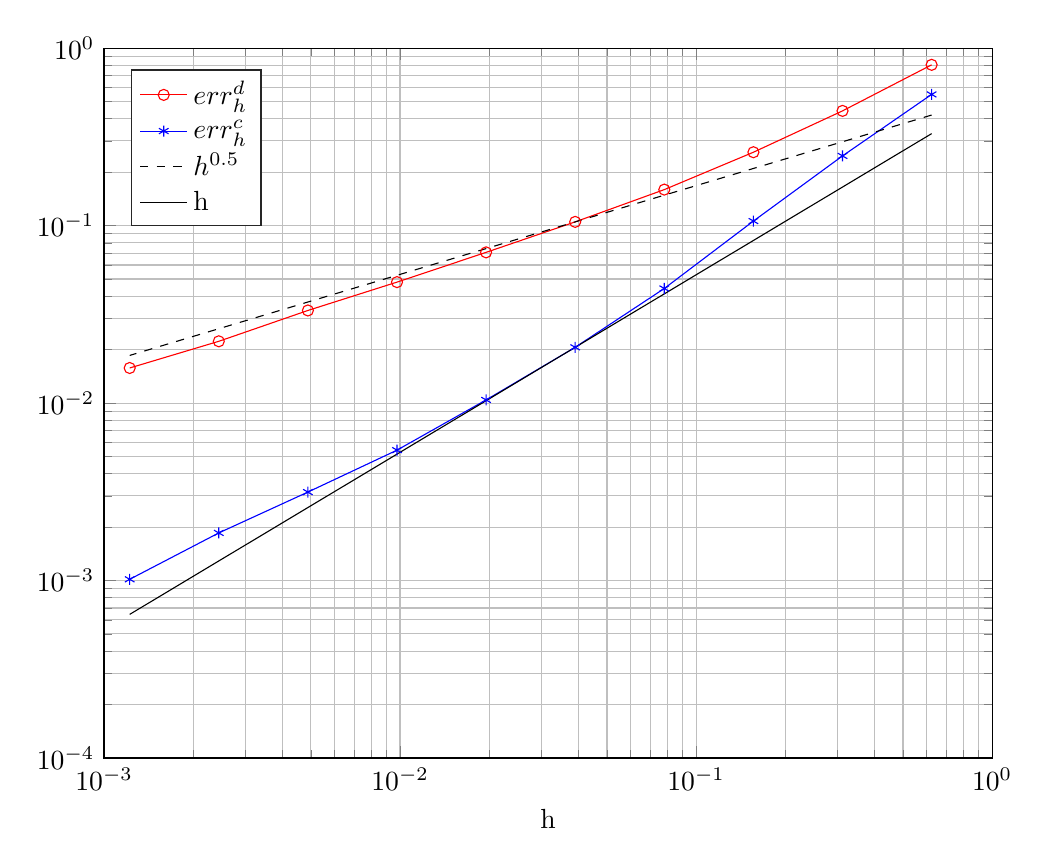
\begin{tikzpicture}

\begin{axis}[%
width=4.44in,
height=3.549in,
at={(0.745in,0.479in)},
scale only axis,
xmode=log,
xmin=0.001,
xmax=1,
xminorticks=true,
xlabel={h},
xmajorgrids,
xminorgrids,
ymode=log,
ymin=0.0001,
ymax=1,
yminorticks=true,
ymajorgrids,
yminorgrids,
axis background/.style={fill=white},
legend style={at={(0.03,0.97)},anchor=north west,legend cell align=left,align=left,draw=white!15!black}
]
\addplot [color=red,solid,mark=o,mark options={solid}]
  table[row sep=crcr]{%
0.625	0.805508168582389\\
0.3125	0.443133168582389\\
0.15625	0.259164418582389\\
0.078125	0.159539418582389\\
0.0390625	0.104953481082389\\
0.01953125	0.0706722310823888\\
0.009765625	0.0480316060823888\\
0.0048828125	0.0332552388948888\\
0.00244140625	0.0222842916292638\\
0.001220703125	0.0157625631136388\\
};
\addlegendentry{$\text{err}_\text{h}^\text{d}$};

\addplot [color=blue,solid,mark=asterisk,mark options={solid}]
  table[row sep=crcr]{%
0.625	0.548758168582389\\
0.3125	0.247101918582389\\
0.15625	0.106070668582389\\
0.078125	0.0442191060823888\\
0.0390625	0.0206175435823888\\
0.01953125	0.0104124654573888\\
0.009765625	0.00542809045738883\\
0.0048828125	0.00315025842613884\\
0.00244140625	0.00185411584801383\\
0.001220703125	0.00101573694176384\\
};
\addlegendentry{$\text{err}_\text{h}^\text{c}$};

\addplot [color=black,dashed]
  table[row sep=crcr]{%
0.625	0.419813924329555\\
0.3125	0.296853272729965\\
0.15625	0.209906962164778\\
0.078125	0.148426636364982\\
0.0390625	0.104953481082389\\
0.01953125	0.0742133181824912\\
0.009765625	0.0524767405411944\\
0.0048828125	0.0371066590912456\\
0.00244140625	0.0262383702705972\\
0.001220703125	0.0185533295456228\\
};
\addlegendentry{$\text{h}^{\text{0.5}}$};

\addplot [color=black,solid]
  table[row sep=crcr]{%
0.625	0.329880697318221\\
0.3125	0.164940348659111\\
0.15625	0.0824701743295553\\
0.078125	0.0412350871647776\\
0.0390625	0.0206175435823888\\
0.01953125	0.0103087717911944\\
0.009765625	0.0051543858955972\\
0.0048828125	0.0025771929477986\\
0.00244140625	0.0012885964738993\\
0.001220703125	0.000644298236949651\\
};
\addlegendentry{h};

\end{axis}
\end{tikzpicture}% }  
        \caption{Killing boundary in $x = 1$}
        \label{fig:KillOneDRough}
    \end{subfigure}
    \begin{subfigure}{0.49\linewidth}
        \centering
        \resizebox{1\linewidth}{!}{% This file was created by matlab2tikz.
%
%The latest updates can be retrieved from
%  http://www.mathworks.com/matlabcentral/fileexchange/22022-matlab2tikz-matlab2tikz
%where you can also make suggestions and rate matlab2tikz.
%
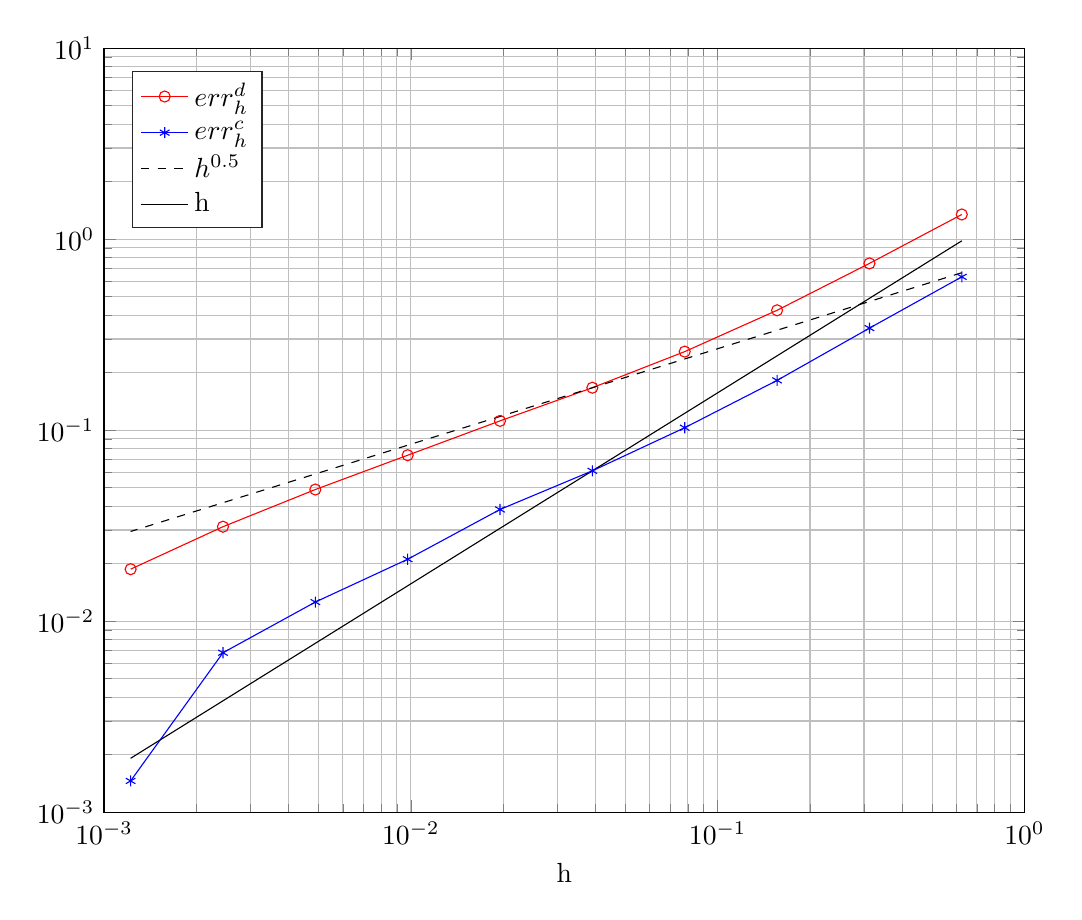
\begin{tikzpicture}

\begin{axis}[%
width=4.602in,
height=3.82in,
at={(0.772in,0.516in)},
scale only axis,
xmode=log,
xmin=0.001,
xmax=1,
xminorticks=true,
xlabel={h},
xmajorgrids,
xminorgrids,
ymode=log,
ymin=0.001,
ymax=10,
yminorticks=true,
ymajorgrids,
yminorgrids,
axis background/.style={fill=white},
legend style={at={(0.03,0.97)},anchor=north west,legend cell align=left,align=left,draw=white!15!black}
]
\addplot [color=red,solid,mark=o,mark options={solid}]
  table[row sep=crcr]{%
0.625	1.34651720868191\\
0.3125	0.746735958681911\\
0.15625	0.424189083681911\\
0.078125	0.257767208681911\\
0.0390625	0.166806271181911\\
0.01953125	0.111831661806911\\
0.009765625	0.0739322477444107\\
0.0048828125	0.0488814664944107\\
0.00244140625	0.0312279020412857\\
0.001220703125	0.0187126432522232\\
};
\addlegendentry{$\text{err}_\text{h}^\text{d}$};

\addplot [color=blue,solid,mark=asterisk,mark options={solid}]
  table[row sep=crcr]{%
0.625	0.634767208681911\\
0.3125	0.342173458681911\\
0.15625	0.182251583681911\\
0.078125	0.102985958681911\\
0.0390625	0.0612633024319106\\
0.01953125	0.0384371305569107\\
0.009765625	0.0210972868069106\\
0.0048828125	0.0125884977444107\\
0.00244140625	0.00683532391628566\\
0.001220703125	0.00145739422878566\\
};
\addlegendentry{$\text{err}_\text{h}^\text{c}$};

\addplot [color=black,dashed]
  table[row sep=crcr]{%
0.625	0.667225084727643\\
0.3125	0.471799381988685\\
0.15625	0.333612542363821\\
0.078125	0.235899690994342\\
0.0390625	0.166806271181911\\
0.01953125	0.117949845497171\\
0.009765625	0.0834031355909553\\
0.0048828125	0.0589749227485856\\
0.00244140625	0.0417015677954777\\
0.001220703125	0.0294874613742928\\
};
\addlegendentry{$\text{h}^{\text{0.5}}$};

\addplot [color=black,solid]
  table[row sep=crcr]{%
0.625	0.98021283891057\\
0.3125	0.490106419455285\\
0.15625	0.245053209727643\\
0.078125	0.122526604863821\\
0.0390625	0.0612633024319106\\
0.01953125	0.0306316512159553\\
0.009765625	0.0153158256079777\\
0.0048828125	0.00765791280398883\\
0.00244140625	0.00382895640199441\\
0.001220703125	0.00191447820099721\\
};
\addlegendentry{h};

\end{axis}
\end{tikzpicture}% }  
        \caption{Reflecting boundary in $x = 1$}
        \label{fig:ReflectOneDRough}
    \end{subfigure}    
    \caption{Orders of convergence for DEM and CEM in the one-dimensional case with $f$ piecewise constant.}
    \label{fig:OrdersOneDRough}
\end{figure}



